
\documentclass[11pt]{book}

\usepackage{AAWS}

%\includeonly{Systems_linear_equationsWS} % UPDATE

%VariablesWS,Variables_and_functionsWS,Tables_and_graphsWS,Rate_of_changeWS,UnitsWS,Metric_system_and_scientific_notationWS,PE1A,PE1B} %Chapter 1

%EquationsWS,First_look_linearWS,First_look_exponentialWS,Using_equationsWS,Approx_solutionsWS,FinanceWS,PE2A,PE2B} %Chapter 2

%Solving_equationsWS,Solving_linear_equationsWS,Solving_linear_inequalitiesWS,Solving_power_equationsWS,Solving_exponential_equationsWS,Solving_quadratic_equationsWS,PE3A,PE3B} %Chapter3

%Closer_look_linearsWS,Modeling_linear_equationsWS,Systems_linear_equationsWS,InterceptsWS,SlopesWS,Fitting_lines_to_dataWS,PE4A,PE4B} %Chapter 4

%Closer_look_exponentialsWS,Modeling_exponential_equationsWS,Exp_growth_decayWS,Growth_factorWS,Linear_vs_exponentialWS,Logistic_growthWS,PE5A,PE5B} %Chapter 5

%Review,Review_exercises,Templates,Formulas} %Review


\begin{document}

%% REVIVE THIS BLOCK
%\frontmatter
%
%\title{\textbf{Workbook for}\\ ~ \\ \begin{Huge} \textsc{Just Enough Algebra}\end{Huge} }
%\author{Dr.\ Suzanne Dor\'ee \\ Professor of Mathematics\\Augsburg College\\Minneapolis, MN 55454}
%\date{2014-15 edition}
%\maketitle
%
%%% 2012 cover GREEN
%%% 2013 cover ORANGE
%%% 2014 cover RED 
%
%\newpage %%%%%%
%
%~\vfill 
%\noindent \textbf{\copyright 2014} Suzanne Dor\'ee  
%
%\noindent All rights reserved.  No part of this publication may be reproduced, stored in a retrieval system, or transmitted, in any form or by any means, electronic, mechanical, photocopying, recording, or otherwise, without the prior written permission of the author.  For information on obtaining permission for use of material in this work, please submit a written request via e-mail to \text{doree@augsburg.edu} or via mail to Suzanne Dor\'ee, Mathematics Department CB 61, Augsburg College, 2211 Riverside Avenue, Minneapolis, MN, 55454. 
%
%\tableofcontents

%%%%%%% END OF BLOCK

%%!TEX root =  A_WS.tex

\setcounter{chapter}{-1}
\chapter{Prelude}



\section{Prelude: Approximation and Rounding} 

\subsection*{Practice exercises}

\begin{enumerate}
\item Round each number up, down, or off to the precision indicated.

\emph{This problem also appears in Section 1.1 \#3.}

\begin{enumerate}
\item My calculations show I need a cross brace around 9.388 feet long. I want the board to be long enough, so round up to the nearest foot.
\vfill
\item Gas mileage is usually rounded down to the nearest one decimal place.  What is the gas mileage for a car measured as getting 42.812 miles per gallon?  What about a car getting 23.09 miles per gallon?
\vfill
\item The population estimate was 4.2 million people, but revised estimates suggest 4,908,229 people.  Report the revised estimate rounded appropriately. What if a different estimate was 4,890,225?  Would that change your answer?
\vfill
\end{enumerate}

\newpage 

\item \begin{enumerate}
\item Callista needs \$117 cash for a mani-pedi at the local salon.  The ATM allows her to withdraw multiples of \$20.  How much money should she withdraw and how many \$20 bills is that? Did you round up, down, or off? 
\vfill
\item Bahari is buying some 8-packs of sparkling water for today's community hour. He expects up to 23 people to be there.  He calculates that he will need $23 \div 8 = 2.875$ 8-packs.  How many 8-packs should he bring?  Did you round up, down, or off? 
\vfill
\item Tzuf has \$20 to buy apples for the new year's celebration.  A bag of apples costs \$3.49.  Tsuf calculates that they can afford $20 \div 3.49 = 5.7306...$ bags. How many bags can they buy? Did you round up, down, or off?  
\vfill
\item Eiji read that life expectancy in the United States is 77.28 years whereas in Japan it is 84.62 years.  How might he describe these life expectancies in (whole) years? Did you round up, down, or off? 
\vfill
\end{enumerate}

\newpage

\item Round off the \underline{calculated number(s)} to give an answer that is reasonable and no more precise than the information given.

\begin{enumerate}
\item The snow removal budget for the city is currently at \$8.3 million but the city council is requesting a reduction of \$1.15 million per year.  We calculate that after three years of cuts, the snow removal budget will be \underline{\$4.8079...} million. 
\vfill
\item A cup of cooked red lentils has around 190 calories and 6.4 grams of dietary fiber, while a cup of cooked chickpeas has around 172 calories and 12.0 grams of dietary fiber.  We calculate that lentils provide \underline{0.03368421...} grams per calorie whereas chickpeas provide \underline{0.06976744...} grams per calorie. 
\vfill
\item \begin{quote} Hibbing [Minnesota] is the former boyhood home of Bob Dylan, basketball great Kevin McHale and the location of the Hull-Rust-Mahoning Open Pit Iron Mine, which has the largest iron-ore pit in the world. Hibbing is also the birthplace of [baseball star] Roger Maris.

\hfill \begin{tiny} (source: http://hibbing.areaconnect.com/)\end{tiny}\end{quote}  

In 2000 the population of Hibbing, Minnesota was reported at just over 17,000 residents. Based on a projected 0.4\% decrease per year, the 2010 population was calculated to be \underline{16,332.110...} people. 
%(In case you are curious, the actual 2010 census count was 17,071 people and the actual 2011 census count was 16,361.  Your reported answer should agree.)
\vfill
\end{enumerate}

\newpage

\item It is easiest to compare the size of decimal numbers when they are written the same precision.  For example, \$1.7 million is more money than \$1.34 million because when we write both numbers to two decimal places we see $$1.7 = 1.70 > 1.34$$  The symbol $>$ means ``greater than;'' it points to the smaller number.  Alternatively, when we expand both numbers we see $$\text{1,700,000}  > \text{1,340,000}$$  

In each story, write all of the decimal numbers given to the same precision and list the numbers from largest to smallest using $>$ signs.

\begin{enumerate}
\item Dawn tested a water sample from her apartment and found 21.19 ppm of sulfate.  She volunteers at a local soup kitchen where the water sample tested at 21.3 ppm.  (The abbreviation \textbf{ppm} stands for ``parts per million.  Not to worry -- sulfate levels below 250 are considered safe for human consumption.)
\vfill
\item There are approximately 1.084 million quarters in circulation in the United States, compared to 1.786 million dimes, 1.6 million \$5 bills,  and 1.42 million \$10 bills.
\vfill

\end{enumerate}

\end{enumerate} % PAUSE

\newpage


\noindent \textbf{When you're done \ldots}

\begin{itemize}
\item [$\Box$] Check your solutions.  Still confused?  Work with a classmate, instructor, or tutor.
\item [$\Box$] Try the \textbf{Do you know} questions.  Not sure?  Read the textbook and try again.
\item [$\Box$] Make a list of key ideas and process to remember under \textbf{Don't forget!}
\item [$\Box$] Do the textbook exercises and check your answers. Not sure if you are close enough? Compare answers with a classmate or ask your instructor or tutor.  
\item [$\Box$] Getting the wrong answers or stuck?  Re-read the section and try again.   If you are still stuck, work with a classmate or go to your instructor's office hours or tutor hours.
\item [$\Box$] It is normal to find some parts of exercises difficult, but if most of them are a struggle, meet with your instructor or advisor about possible strategies or support services.
\end{itemize}





\bigskip

\noindent \textbf{Do you know \ldots}

\begin{enumerate}[(a)]
\item What the symbol for ``approximately equal to'' is? \vfill
\item Why an approximate answer is often as good as we can get? \vfill
\item What the term ``precisely'' refers to? \vfill
\item What the saying ``I'd rather be approximately right than precisely wrong'' means? \vfill
\item What the difference is between rounding off, rounding up, and rounding down? \vfill
\item When to round your answer, and when to round your answer up or down (instead of off)? \vfill
\item How to round a decimal to the nearest whole number? \vfill  To one decimal place? \vfill  To two decimal places? \vfill
\item How precisely to round an answer? \vfill
\item How to compare sizes of decimal numbers? \vfill
\item What the symbol for ``greater than'' is? \vfill
\end{enumerate}

\noindent \textbf{Don't forget!}
\vfill \vfill \vfill

%%DO I want to add the symbols for less than, greater than or equal to, less than or equal to????





\section{Prelude: Arithmetic Operations} 

\subsection*{Practice exercises}

On each problem, write down what you enter into your calculator and don't forget to write the units on your final answer. You are welcome to calculate the answer step-by-step but also challenge yourself to figure out the answer all at once, not hitting = on your calculator until the very end.

\begin{enumerate}

\item Tensia loves to garden but can't quite keep up with how many cucumbers are growing.  
\begin{itemize}
\item At the start of the week she had 8 cucumbers in her refrigerator. 
\item Her son, N\'estor took 3 home with him after dinner on Monday.  
\item Tensia harvested another 7 cucumbers on Wednesday.  
\item Her neighbor Sarah graciously took 4 cucumbers to make pickles.  
\item Tensia herself ate 2 cucumbers during the week.  
\end{itemize}
How many cucumbers does she have left over?  \vfill

\item Brent's landlord charges \$15 per day for late rent.
\begin{enumerate} 
\item What will Brent's late fee be if is 6 days late paying his rent? 
\vfill  
\item If Brent got a bill showing \$195 in late fees, how many days late did he pay his rent? 
\vfill
\end{enumerate}

\newpage 

\item There are 2,624 students at a local university.

\begin{enumerate}
\item About $\frac{3}{4}$ of those students live on or within a mile of campus. How many students live on or within a mile of campus?   
\vfill 
\item The university wants to support 40 hours a week of onsite tutoring (in mathematics, writing, etc.) for each the 32 weeks that classes are in session.  It costs about \$18/hour to pay the tutors and staff administrators.  What is the total cost of tutoring? 
\vfill
\item The university is considering adding a tutoring fee to cover the cost of tutoring.  If they wanted to cover the total cost of tutoring, what would the cost per student be?
\vfill
\end{enumerate}


\item A truck hauling grass seed weighs 3,900 pounds when it is empty. Each bag of seed it carries weighs 4.2 pounds.  The \textbf{gross weight} of the truck is the total weight including the truck and the bags of seed. 

\hfill \emph{Story also appears in 2.1 \#1, 3.2 \#1, and 3.1 \#1}
\begin{enumerate}
\item How much does 1,300 bags of grass seed weigh? 
\vfill
\item What is the gross weight of the truck if it carries 1,300 bags of grass seed?
\vfill
\item You probably entered this calculation as $1300 \times 4.2 = + 3900=$.  What happens if you skip the middle = sign and enter $1300 \times 4.2 + 3900$ instead?
\vfill
\item What answer does your calculator give you if you enter $3900 + 4.2 \times 1300$ instead?
\vfill
\item What does part (d) tell you about which operation your calculator did first: the $+$ or the $\times$? 
\vfill
\end{enumerate}

\end{enumerate} % PAUSE

\newpage


\noindent \textbf{When you're done \ldots}

\begin{itemize}
\item [$\Box$] Check your solutions.  Still confused?  Work with a classmate, instructor, or tutor.
\item [$\Box$] Try the \textbf{Do you know} questions.  Not sure?  Read the textbook and try again.
\item [$\Box$] Make a list of key ideas and process to remember under \textbf{Don't forget!}
\item [$\Box$] Do the textbook exercises and check your answers. Not sure if you are close enough? Compare answers with a classmate or ask your instructor or tutor.  
\item [$\Box$] Getting the wrong answers or stuck?  Re-read the section and try again.   If you are still stuck, work with a classmate or go to your instructor's office hours or tutor hours.
\item [$\Box$] It is normal to find some parts of exercises difficult, but if most of them are a struggle, meet with your instructor or advisor about possible strategies or support services.
\end{itemize}





\bigskip

\noindent \textbf{Do you know \ldots}

\begin{enumerate}[(a)]
\item When to add, subtract, multiply, or divide numbers? \vfill
\item What is the difference between subtraction and negation? \vfill % pun intended :-)
\item How to add, subtract, negate, multiply, and divide on a calculator? \vfill
\item How multiplication is related to addition? \vfill
\item What the term ``per'' indicates? \vfill
\end{enumerate}

\noindent \textbf{Don't forget!}
\vfill \vfill \vfill






\section{Prelude: Percentages} 

\subsection*{Practice exercises}

On each problem, write down what you enter into your calculator and don't forget to write the units on your final answer. You are welcome to calculate the answer step-by-step but also challenge yourself to figure out the answer all at once, not hitting = on your calculator until the very end.


%For exercises look at textbook: 2.2 + 3.4 + Chapter 5
%
%For workbook look at workbook: 2.2 + 3.4 + Chapter 5
%Percents
%Low-fat milk or fat in ground beef 
% RDA of nutrients
%save percentage for goalie in hockey or completion percentage quarterback football
%First gen students or voters for candidate
%
%Percent increase
%Tip on purchase -- have them check Thang's tip
%Interest rate n loan
%Inflation price of food or rent or rent control caps
%Population
%
%Percent decrease
%Ice cap coverage 

\begin{enumerate}

\item As I write this problem, the population of the world is 8,056,959,718 people (just over 8 billion).  It changes by the second, so let's use the round figure of 8,100,000,000.
\begin{enumerate}
\item I read that the population of Brazil accounts for 2.69\% of the world's population.  According to that report, what is the population of Brazil?  Round your answer to the nearest million.  \vfill
\item If the population of the United States is currently around 334,000,000, what percentage of the world's population is in the United States? \vfill
\end{enumerate}

\item In Minneapolis, apartment rent is expected to increase by 16\% next year. \begin{enumerate}
\item Astra lives in a 1-bedroom apartment where they pay \$825 per month in rent.  If their rent increased by 16\% what would their new rent be? \vfill
\item Lucky for Astra, their building is subject to rent stabilization laws and so their rent cannot increase by more than 3\%. What would their new rent be? \vfill
\end{enumerate}

\newpage

\item The corner by my house is dangerous.  One year there were 14 accidents there.  The neighbors got together and petitioned to have 4-way stop signs installed.  
\begin{enumerate}
\item The city estimated that the installed stop signs would reduce accidents at least 40\%.  If that happens, how many accidents would we expect the next year? \vfill
\item The national average shows that the new signs could reduce accidents up to 62\%.  If that happens instead, how many accidents would we expect the next year? \vfill
\item If there were 6 accidents the next year, is that in the range you figured out? What percent decrease does that correspond to? \vfill 
\end{enumerate}

\item My savings account earns a modest amount of interest, the equivalent of .75\% annually.  I have \$12,392.18 in the account now.  \hspace{.7 in} \emph{Story also appears in 2.2\#4}
\begin{enumerate}
\item How much interest will I earn this year? \vfill
\item How much will my account balance be at the end of the year? \vfill
\end{enumerate}

\end{enumerate} % PAUSE

\newpage


\noindent \textbf{When you're done \ldots}

\begin{itemize}
\item [$\Box$] Check your solutions.  Still confused?  Work with a classmate, instructor, or tutor.
\item [$\Box$] Try the \textbf{Do you know} questions.  Not sure?  Read the textbook and try again.
\item [$\Box$] Make a list of key ideas and process to remember under \textbf{Don't forget!}
\item [$\Box$] Do the textbook exercises and check your answers. Not sure if you are close enough? Compare answers with a classmate or ask your instructor or tutor.  
\item [$\Box$] Getting the wrong answers or stuck?  Re-read the section and try again.   If you are still stuck, work with a classmate or go to your instructor's office hours or tutor hours.
\item [$\Box$] It is normal to find some parts of exercises difficult, but if most of them are a struggle, meet with your instructor or advisor about possible strategies or support services.
\end{itemize}





\bigskip

\noindent \textbf{Do you know \ldots}

\begin{enumerate}[(a)]
\item What the words ``per'' and ``cent'' mean in the word ``percent.'' \vfill
\item How to convert a fraction or decimal to a percent? \vfill
\item How to convert a percent to a decimal? \vfill
\item How to calculate a percentage of a number? \vfill
\item How to calculate the result of a percent increase or a percent decrease? \vfill
%\item How to use the distributive property to do percent increase or percent decrease using a single multiplication? %\vfill
\end{enumerate}

\noindent \textbf{Don't forget!}
\vfill \vfill \vfill






\section{Prelude: Order of Operations} 

\subsection*{Practice exercises}

On each problem, write down what you enter into your calculator and don't forget to write the units on your final answer.  Challenge yourself to use one-line calculations. You are welcome to calculate the answer step-by-step to check.

\begin{enumerate}

\item  \emph{Story also appears in 1.2 \#4, 2.1 \#4, and 4.2 \#2}

\begin{enumerate}
\item A mug of coffee costs \$3.45 at Juan's favorite cafe.  If Juan orders 25 coffees each month, how much will he pay (total) for the month?
\vfill
\item The cafe offers a deal each month, where if you buy their \$10 discount card, then you only pay \$2.90 per mug of coffee during the month. If Juan buys the discount card and orders 25 coffees, how much will he pay (total) for the month?  
\vfill
\item Comparing answers to parts (a) and (b) is it worthwhile for Juan to buy the card? Discuss.
\vfill
\end{enumerate}

\item ``Rose gold'' is a mix of gold and copper. 

\hfill \emph{Story also appears in 2.3 \#2 and 4.1 Exercises}
\begin{enumerate}
\item If we mix 2 grams of gold with 2 grams of copper, what is the percentage of gold in the resulting alloy?
\vfill
\item If instead we mix 2 grams of gold with 7 grams of copper, what is the percentage of gold in the resulting alloy?
\vfill
\end{enumerate}
  
\newpage

\item \emph{Stories also appear in 4.3 \#3}
\begin{enumerate}
\item Vanessa's doctor put her on a sensible diet and exercise plan to get her back to a healthy weight.  She currently weighs 213 pounds. She will need to lose an average of 1.25 pounds a week to reach her goal weight in a year.  What is her goal weight?  Use $1 \text{ year} =  52 \text{ weeks}$. \vfill
\item Since she has been pregnant, Zoe has gained the recommended \nicefrac{1}{2} pound per week.  She weighed 153 at the start of her pregnancy.  What does she weigh now at 30 weeks pregnant? \vfill
\end{enumerate}

\item \emph{Stories also appear in 4.3 \#3}
\begin{enumerate}
\item Jerome has gained weight since he took his power training to the next level ten weeks ago, at the rate of around 1 pound a week.  He is now 198 pounds.  What was his original weight? \vfill
\item After the past 6 weeks of terrible migrane headaches, Carlos is down to 158 pounds.  He has lost 4 pounds a week. What did Carlos weigh when 6 weeks ago? \vfill
\end{enumerate}

\end{enumerate} % PAUSE

\newpage


\noindent \textbf{When you're done \ldots}

\begin{itemize}
\item [$\Box$] Check your solutions.  Still confused?  Work with a classmate, instructor, or tutor.
\item [$\Box$] Try the \textbf{Do you know} questions.  Not sure?  Read the textbook and try again.
\item [$\Box$] Make a list of key ideas and process to remember under \textbf{Don't forget!}
\item [$\Box$] Do the textbook exercises and check your answers. Not sure if you are close enough? Compare answers with a classmate or ask your instructor or tutor.  
\item [$\Box$] Getting the wrong answers or stuck?  Re-read the section and try again.   If you are still stuck, work with a classmate or go to your instructor's office hours or tutor hours.
\item [$\Box$] It is normal to find some parts of exercises difficult, but if most of them are a struggle, meet with your instructor or advisor about possible strategies or support services.
\end{itemize}





\bigskip

\noindent \textbf{Do you know \ldots}

\begin{enumerate}[(a)]
\item How a calculator will evaluate an expression that has several different operations, such as $2.1 + 7 \times 1.1$? \vfill
\item What is the order of operations in general?  \vfill
\item A good way to remember PEMDAS? \vfill
\item Why you need to know what the order of operations is? \vfill
\item When might you need to override the order of operations? \vfill
\item How to override the order of operations using parentheses? \vfill
\end{enumerate}

\noindent \textbf{Don't forget!}
\vfill \vfill \vfill






\section{Prelude: Fractions} 

\subsection*{Practice exercises}
%%\emph{Story also appears in 1.2 \#4, 2.1 \#4, and 4.2 \#2}

\begin{enumerate}

\item There are 2,624 students at a local university.  
\begin{enumerate}
\item Of those students, 673 of those students placed into this algebra class.  What fraction of students placed into algebra? 
\vfill
\item The Dean said that approximately 1 in 4 students, or $\frac{1}{4}$ of all students, placed into algebra.  Is that correct?  Check by determining if your answer to part (a) $\approx \frac{1}{4}$ by comparing decimal approximations. 
\vfill
\end{enumerate}

\item Gas mileage is usually rounded down to the nearest one decimal place. Gas mileage is measured in miles per gallon (mpg).
\begin{enumerate}
\item Xu does gig work delivering take-out food from local restaurants.  He started the week with a full tank of gas and drove 319 miles.  When he went to fill the tank, he needed 11.3 gallons. What was Xus gas mileage?
\vfill
\item Margaret and Cathy are on a cross-country trip.  They've driven from Minnesota to Maine (approximately 1,430 miles).  They have bought gas a few times along the way:  12.7 gallons, then 14.0 gallons, then 13.1 gallons, and then 12.4 gallons.  What was Margaret and Cathy's gas mileage? 
\vfill
\item How could you do the calculation in part (b) one line on your calculator by using parentheses?
\vfill
\end{enumerate}

\newpage %%%%%

\item In January 2015, Graham had 47 albums in his vinyl collection.  By September 2023 (that's 8 years, 9 months later), he had 783 albums.  Approximately how many albums per month did Graham buy?
\begin{enumerate}
\item Figure out the answer step by step.
\vfill
\vfill
\item Now try to combine all of your calculations into one line on your calculator.  Hint:  write as a fraction first.
\vfill
\end{enumerate}

\item It took Mariam 3 hours to complete the reading for her Religion class. The reading was 102 pages long.  
\begin{enumerate}
\item How fast did she read measured in pages per hour? Write the answer as a fraction and as a decimal. 
\vfill
\item Reading speed is often measured in words per minute.  Assuming there are approximately 500 words per page, calculate Mariam's reading speed step by step.
\vfill
\vfill
\item How could you do the calculation in part (b) one line on your calculator by using parentheses? Hint: the ``hours'' cancel! 
\vfill 
\end{enumerate}

\end{enumerate}

\newpage %%%%%


\noindent \textbf{When you're done \ldots}

\begin{itemize}
\item [$\Box$] Check your solutions.  Still confused?  Work with a classmate, instructor, or tutor.
\item [$\Box$] Try the \textbf{Do you know} questions.  Not sure?  Read the textbook and try again.
\item [$\Box$] Make a list of key ideas and process to remember under \textbf{Don't forget!}
\item [$\Box$] Do the textbook exercises and check your answers. Not sure if you are close enough? Compare answers with a classmate or ask your instructor or tutor.  
\item [$\Box$] Getting the wrong answers or stuck?  Re-read the section and try again.   If you are still stuck, work with a classmate or go to your instructor's office hours or tutor hours.
\item [$\Box$] It is normal to find some parts of exercises difficult, but if most of them are a struggle, meet with your instructor or advisor about possible strategies or support services.
\end{itemize}





\bigskip

\noindent \textbf{Do you know \ldots}

\begin{enumerate}[(a)]
\item How we represent a part of a whole as a fraction? \vfill
\item How to multiply fractions?  \vfill
\item What``canceling'' a factor means? \vfill
\item How fractions are related to division? \vfill
\item How to calculate the decimal approximation of a fraction? \vfill
\item How to compare two fractions using their decimal approximations? \vfill
\item How the units of a fraction are determined?  \vfill
\item When we need to use parentheses around the top (numerator) and bottom (denominator) to evaluate a fraction? \vfill
\end{enumerate}

\noindent \textbf{Don't forget!}
\vfill \vfill \vfill




 
\include{Prelude 0.6 Powers and Roots WS}

\section{Prelude: Algebraic Notation} 

\subsection*{Practice exercises}

\begin{enumerate}

\item Since she has been pregnant, Zoe has gained the recommended $\frac{1}{2}$ pound per week. She weighted 153 pounds at the start of her pregnancy.  That means when she is $W$ weeks pregnant, that Zoe weighs $$153 + \frac{1}{2}W$$
What does this expression say Zoe will weigh when she's 40 weeks pregnant? 

\hfill \emph{Story also appears in 0.4 \#3  and 4.3 \#3} \vfill

\item Jody is using small wooden balls to make noses for her knitted gnomes.  She figured out that she can calculate the weight of each ball (in ounces) as $.2 \times B \land 3$.  Write this expression in algebraic notation. 

\hfill \emph{Story also appears in 0.6 \#1}
\vfill

\newpage %%%%%

\item Astra lives in a 1-bedroom apartment where they pay \$825 per month in rent. Thanks to new rent stabilization laws, Astra's rent can only increase 3\% per year.  That means after $Y$ years, their rent will be at most $$825(1.03^Y)$$  What does this expression say her rent could be in 5 years? 

\hfill \emph{Story also appears in 0.3 \#2} \vfill

\item  ``Rose gold'' is a mix of gold and copper.  If we mix 2 grams of gold with $C$ grams of copper, the percentage of the resulting alloy that is gold is given by the expression $$\frac{200}{2 +C}$$
What does this expression say the percentage of gold will be if we add 7 grams of copper?

 \hfill \emph{Story also appears in 0.4 \#2, 2.3 \#2, and 4.1 Exercises} \vfill

\end{enumerate}

\newpage %%%%%


\noindent \textbf{When you're done \ldots}

\begin{itemize}
\item [$\Box$] Check your solutions.  Still confused?  Work with a classmate, instructor, or tutor.
\item [$\Box$] Try the \textbf{Do you know} questions.  Not sure?  Read the textbook and try again.
\item [$\Box$] Make a list of key ideas and process to remember under \textbf{Don't forget!}
\item [$\Box$] Do the textbook exercises and check your answers. Not sure if you are close enough? Compare answers with a classmate or ask your instructor or tutor.  
\item [$\Box$] Getting the wrong answers or stuck?  Re-read the section and try again.   If you are still stuck, work with a classmate or go to your instructor's office hours or tutor hours.
\item [$\Box$] It is normal to find some parts of exercises difficult, but if most of them are a struggle, meet with your instructor or advisor about possible strategies or support services.
\end{itemize}





\bigskip

\noindent \textbf{Do you know \ldots}

\begin{enumerate} [(a)]
\item Where multiplication can be hidden in algebraic notation? \vfill
\item How powers are written in algebraic notation? \vfill
\item How division is written in algebraic notation? \vfill
\item What the word evaluate means? \vfill
\item How to evaluate an algebraic expression on your calculator? \vfill
\end{enumerate}

\noindent \textbf{Don't forget!}
\vfill \vfill \vfill






\section{Prelude: Scientific Notation} 

\subsection*{Practice exercises}

\begin{enumerate}

\item In each story, write out the highlighted numbers (with all the zeros).
\begin{enumerate}
\item Melvin was looking populations based on the 2020 Census and saw the population of Saint Paul, MN listed as $\mathbf{3.10942 \times 10^{5}}$ \textbf{people}. Hint:  you can check the answer to this part by evaluating on your calculator. \vfill
\item The gross domestic product (GDP) measures the market value of all final goods and services produced by an economy. The United States GDP is approximately $\mathbf{\$2.332 \times 10^{13}}$.
\hfill \emph{Story also appears in 1.5 \#1} \vfill
\item The Earth weighs approximately $\mathbf{5.972 \times 10^{24}}$ \textbf{kilograms}.

\hfill \emph{Story also appears in 1.5 \#3} \vfill
\end{enumerate}

\item In each story, write out the highlighted numbers (with all the zeros).
\begin{enumerate}
\item Alpaca have very fine hairs (which can be spun into yarn to make very soft sweaters).  The width of an alpaca hair is around $\mathbf{2.5 \times 10^{-7}}$ \textbf{meters}. Hint:  you can check the answer to this part by evaluating on your calculator. \vfill
\item A dust particle weighs approximately $\mathbf{7.53 \times 10^{-10}}$ \textbf{grams}.

\hfill \emph{Story also appears in 1.5 \#2} \vfill
\item  A proton (part of an atom) has mass of about $\mathbf{1.67262 \times 10^{-27}}$ \textbf{kilograms}.

\hfill \emph{Story also appears in 1.5 \#7} \vfill
\end{enumerate}

\newpage %%%%%%

\item In each story, evaluate the number and report your answer in scientific notation.
\begin{enumerate}
\item Bunnies, bunnies, everywhere.  In 2007 there were 1800 and that number was predicted to increase 13\% each year.  I was trying to predict the number of rabbits in 2023 (after 16 years) but I accidentally typed in 166 years by mistake $$1800 \ast 1.13 \wedge 166=$$
Report the answer I got in scientific notation.  (Yes, this is a gigantic number.  The exponential model I used doesn't actually make sense for that many years.)   

\hfill \emph{Story also appears in 2.1 \#2 and 5.1 \#3}\vfill
\item A signal is sent down a fiber optic cable.  Its strength decreases by 2\% each mile it travels. We can calculate the signal strength after 1000 miles by evaluating $$.98 \wedge 1000=$$
Report the answer you get in scientific notation. (Yes, this is a teeny number.  In reality there would be signal booster installed along the route.)

\hfill \emph{Story also appears in 5.2 \#1} \vfill
\end{enumerate}

\item In each story, write out the highlighted number (with all the 0s).  Note that \textbf{million} is short for $\times 10^6$, \textbf{billion} is short for $\times 10^9$, and \textbf{trillion} is short for $\times 10^{12}$.
\begin{enumerate}
\item There are approximately \textbf{1.084 million quarters} in circulation in the United States. \hfill \emph{Story also appears in 0.1 \#4} \vfill
\item The population of the world is approximately  \textbf{8.1 billion people}. 

\hfill \emph{Story also appears in 0.3 \#1} \vfill

\item One way that the United States government borrow money is Treasury bonds (T-bonds).  %For example, you might pay \$600 for a \$1000 T-bond that matures in 10 years.  That means you paid \$600 now and in 10 years the government will pay you \$1000.  
There are approximately 
 \textbf{\$24 trillion} worth of T-bonds currently.  \vfill
\end{enumerate}

\end{enumerate}


\newpage %%%%%


\noindent \textbf{When you're done \ldots}

\begin{itemize}
\item [$\Box$] Check your solutions.  Still confused?  Work with a classmate, instructor, or tutor.
\item [$\Box$] Try the \textbf{Do you know} questions.  Not sure?  Read the textbook and try again.
\item [$\Box$] Make a list of key ideas and process to remember under \textbf{Don't forget!}
\item [$\Box$] Do the textbook exercises and check your answers. Not sure if you are close enough? Compare answers with a classmate or ask your instructor or tutor.  
\item [$\Box$] Getting the wrong answers or stuck?  Re-read the section and try again.   If you are still stuck, work with a classmate or go to your instructor's office hours or tutor hours.
\item [$\Box$] It is normal to find some parts of exercises difficult, but if most of them are a struggle, meet with your instructor or advisor about possible strategies or support services.
\end{itemize}





\bigskip

\noindent \textbf{Do you know \ldots}

\begin{enumerate} [(a)]
\item What million, billion, and trillion mean? \vfill
\item Why scientific notation is used? \vfill 
\item The standard format for scientific notation? \vfill 
\item That a positive exponent corresponds to a big number and a negative exponent corresponds to a tiny number? \vfill
\item How to convert from scientific notation to decimal? \vfill
\item How your calculator reports numbers in scientific notation, and what (might be) different when you're reporting that number? \vfill
\end{enumerate}

\noindent \textbf{Don't forget!}
\vfill \vfill \vfill






\section{Prelude: Logarithms} 

\subsection*{Practice exercises}

\begin{enumerate}

\item The number of bacteria in a dish increases 10-fold each day.   Note: 10-fold means $\times 10$.  Suppose we had 1 microliter of bacteria at the start of the first day.  That means after $D$ days there will be $10^D$ microliters of bacteria.
\begin{enumerate}
\item How many bacteria (in microliters) will there be after 1 day?  After 2 days? After 3 days?
\vfill
\item In how many days will the bacteria have reached 1 liter, which is million microliters?   \vfill
\item How can we use logs to find the answer?\vfill
\end{enumerate}

\item The problem continues \ldots
\begin{enumerate}
\item How many days(from the start) does it take to reach the 25 millilter capacity of the petri dish, which is 25,000 microliters?  Guess and check to find the answer to 1 decimal place. \vfill
\item How can we use logs to find the answer? \vfill
\item Convert your answer to days \& hours format (meaning d days and h hours). \vfill
\end{enumerate}

%\item The world's population is increasing 10-fold every 250 years.  In 2000 the world's population was approximately 6.1 billion.
%\begin{enumerate}
%\item According to this model, what will the world's population be in the year 2250? That's 250 years later. \vfill
%\item What will the world's population be in the year 2500? That's another 250 years later. \vfill
%\item When will the world's population pass 1 trillion people?  That's 1,000 billion so we're looking for the number $N$ where $6.1 \ast 10^N =\text{1,000}$.  Note: in part (a) we had $N=1$ and in part (b) we had $N=2$. Guess to find the value of $N$ correct to one decimal place. \vfill \vfill
%\item Use logs to find the value of $N$.As we'll see later, the answer is $\displaystyle \log(\frac{1000}{6.1})$ \vfill
%\item What year does that value of $N$ represent?  Recall that $N$ counts the multiple of 250 years, so the year should be $2000 + 250N$. \vfill
%\end{enumerate}

\newpage %%%%%%

\item The equation $pH = -\log(H^+)$ tells us the pH of a substance (on a scale from 0 to 14) based on its molar hydrogen ion concentration $H^+$.  Don't let the notation here scare you: $pH$ is a single quantity and $H^+$ has nothing to do with exponents or adding. 

For example, lemon juice has $H^+= .0025$ and so the pH of lemon juice is 
$$-\log(.0025) = \text{(-)} \log(.0025) = 2.6020599913 \approx 2.6$$

\begin{enumerate}
\item Coca-cola has $H^+= .000~398$.  Find the pH of orange juice. Note: the funny spaces are to help you read the number.\vfill
\item Hair shampoo has $H^+= .000~003~162$  Find the pH of hair shampoo. \vfill
\item Household bleach has $H^+=1.1 \times 10^{-13}$  Find the pH of bleach. \vfill
\item Materials with pH values between 0-5 are \textbf{acidic}, between 9-14 are \textbf{basic}, and between 5-7 are \textbf{neutral}.  Which of the above materials are acid, basic, and neutral?  \vfill
 \end{enumerate}
 

\item In Minneapolis, apartment rent is expected to increase by 16\% next year.  \

\hfill \emph{Story also appears in 0.3 \#2}
\begin{enumerate}
\item Astra lives in a 1-bedroom apartment where they pay \$825 per month in rent.  If their rent increased by 16\% in how many years would their rent be doubled to \$1,650.  As we'll see later, the answer is $\displaystyle \frac{\log(2)}{\log(1.16)}$.  Don't forget to the close the parentheses.  
\vfill
\item Lucky for Astra, their building is subject to rent stabilization laws and so their rent cannot increase by more than 3\%. In how many years would their rent double under this cap?  The answer is $\displaystyle \frac{\log(2)}{\log(1.03)}$.\vfill
\end{enumerate}



\end{enumerate}


\newpage %%%%%


\noindent \textbf{When you're done \ldots}

\begin{itemize}
\item [$\Box$] Check your solutions.  Still confused?  Work with a classmate, instructor, or tutor.
\item [$\Box$] Try the \textbf{Do you know} questions.  Not sure?  Read the textbook and try again.
\item [$\Box$] Make a list of key ideas and process to remember under \textbf{Don't forget!}
\item [$\Box$] Do the textbook exercises and check your answers. Not sure if you are close enough? Compare answers with a classmate or ask your instructor or tutor.  
\item [$\Box$] Getting the wrong answers or stuck?  Re-read the section and try again.   If you are still stuck, work with a classmate or go to your instructor's office hours or tutor hours.
\item [$\Box$] It is normal to find some parts of exercises difficult, but if most of them are a struggle, meet with your instructor or advisor about possible strategies or support services.
\end{itemize}





\bigskip

\noindent \textbf{Do you know \ldots}

\begin{enumerate} [(a)]
\item What a logarithm (base 10) means? \vfill
\item How to evaluate logarithms (base 10) on a calculator? \vfill
\item Which size numbers have a positive log and which have a negative log (base 10)? \vfill
\item The connection between logarithms (base 10) and scientific notation. \vfill
\end{enumerate}

\noindent \textbf{Don't forget!}
\vfill \vfill \vfill






%%!TEX root =  A_WS.tex

\section*{Preface to workbook}
\addcontentsline{toc}{section}{Preface to workbook}

In 1994, my colleagues at Augsburg College and I had a vision for a new course to replace our intermediate algebra course.  We wanted a college level course that would serve primarily as preparation for quantitative courses across the curriculum. The framing question that led to our curricular adventure of the past nearly two decades was 
\begin{quote}  What algebra do college students need to know, and how can we make it relevant to their future studies, their lives as citizens, and their everyday life?
\end{quote}
From these questions \emph{Just enough algebra} was born.  

As you will see, everything we do is in some applied context.  
Our choice to focus primarily on linear and exponential models; to emphasize verbal, numerical, and graphical interpretation of functions; and to include only the most essential symbolic techniques  align well with curricular guides from the MAA\footnote{\emph{Curricular Guide}, Committee on the Undergraduate Mathematics Program (CUPM) and \emph{Curriculum Foundations Project:  Voices of the Partner Disciplines}, Curriculum Renewal Across the First Two Years (CRAFTY), Mathematical Association of America (MAA), 2004 and CRAFTY's \emph{Recommendations for College Algebra}, 2007} 
and AMATYC\footnote{\emph{Crossroads in Mathematics Standards for Introductory College Mathematics Before Calculus}, American Mathematical Association of Two-Year Colleges (AMATYC), 1995 and the follow up ``Beyond Crossroads'' report, AMATYC, 2006.}.
More importantly, it works.  Student learn a lot in this course.  They are ready for what comes next.  And, they enjoy it.


\section*{To the student}
This workbook is written for you.  Read the narrative examples in the accompanying textbook, listen to examples in class, try the practice exercises here in the workbook, check with classmates or your instructor, then work the exercises in the textbook, then chat with classmates again, then do more problems, \ldots.  Well, you get the idea:  the best way to learn mathematics is to do it yourself.  I hope you enjoy the course.  I know you will learn a lot of useful algebra.  I believe it will change how you see mathematics.

\section*{To the instructor}
At Augsburg College we usually begin class with a brief entrance quiz on the previous section or some other activity to review.  Next, the instructor presents one well-chosen example illustrating the main theme of the new section and works through that problem on the board, with students helping with the calculations along the way. For me, part of the fun of teaching this course is creating lecture examples from the day's news or connected to popular culture, but in a pinch there is often an exercise in the textbook that can be used for that purpose.  

Then, students work with a classmate on the practice exercises in this workbook while the instructor circulates to answer questions and help students stay on task.  The first exercise in each section of the workbook parallels the main theme, but I've deliberately left some variations for students to discover in the second and third exercises.  The fourth exercise varies, but often wanders a bit off the main path.  We normally budget 30 minutes of class time for student work.  This timing allows nearly all students to finish at least the first exercise and check their solution; most students finish two or three exercises; and even our fastest students rarely finish all four exercises in under 30 minutes.

 After class students are expected to finish the section in the workbook, try the \textbf{Do you know} questions, read the textbook narrative example, and try some of the exercises in the textbook.  Hand-written solutions to the practice exercises in this workbook are available (in electronic format) for students to check their work, whether in class or at home.  Answers to the textbook exercises appear in the back of the textbook.  

My greatest success in teaching this course has been to give students room to figure things out for themselves, so try to resist the temptation to show them one of everything.   Listen to your students and help them understand the algebra in their own vocabulary.  You will be impressed.

\section*{Acknowledgments}

Thanks, first, to the thousands of students who have taken this course.  Their creative approaches to learning mathematics; their unedited criticism and challenge; their often surprising enthusiasm for the course; their patience tried by countless typos and outright mistakes; and their perpetually novel insights have humbled me and challenged everything I thought I knew about teaching and learning mathematics.  They have inspired me time and time again.  I am grateful that they have allowed me to make a difference in their lives.

Thanks, next, to my mathematics colleagues at Augsburg: Mathew Foss (now at North Hennepin Community College), who taught from the very first edition of the textbook back in 1997 and who collaborated in writing earlier versions; Matt Haines, Alyssa Hanson, Rich Flint, and the dozens of other professors who have taught the course over the years from various earlier editions of the textbook; John Zobitz and Jody Sorensen, who edited and created more exercises for the 2012 edition;  and student helpers Ashley Gruhlke and Emma Winegar.

Thanks, also, to my colleagues across campus for allowing us to try something completely different and to my mathematics colleagues nationally for spurring me on.  During the first few years I taught this course from \emph{Using algebra} by Ethan Bolker.  Much of my approach and probably more examples or exercises than I realize are derived from his vision and from the subsequent text by his colleagues Linda Kime and Judy Clark at University of Massachusetts, Boston.  

A special thanks to Dean Barbara Farley, Augsburg's Center for Teaching and Learning, and Augsburg's Undergraduate Research and Graduate Opportunity program for supporting my work through sabbaticals, travel grants, and summer research grants for both me and students.


 
%
%\mainmatter
%
%
\chapter{Variables}

 
%	
\section{Variables and functions  -- Practice exercises}
\begin{enumerate}

\item A 32 pound bag of dog food costs \$29.97, but a 8 pound bag costs \$11.28.  
\begin{enumerate}
\item  Identify and name the variables, including the units. \vfill
\item Which variable is dependent and which is independent? \vfill
\item What might a 16 pound bag of dog food cost? Explain the reasoning behind your guess.  
\end{enumerate} %MIGHT DO FOLLOW UP IN 4.4 or 5.4
 \vfill \vfill
 
\newpage %%%%%%%%%

\item Rent in the Riverside Neighborhood is expected to increase 7.2\% each year.  Average rent for an apartment is currently \$830 per month.  \hfill \emph{Story also appears in 3.4 \#3} 
\begin{enumerate}
\item Identify and name the variables, including the units. \vfill
\item Explain the dependence using a sentence of the form ``\underline{~\quad} is a function of \underline{~\quad}'' \bigskip
\item Which number is a constant in this story:  the percent increase (7.2) or the apartment rent (830)? \bigskip
\item What is a realistic domain for this function?  That means, for how many years might this sort of increase in rent continue?   Express your answer as an inequality. \vfill
\item What is the average rent expected to be in 1 year?  In 2 years?  In 3 years?  Note that $$7.2\% = \frac{7.2}{100} = 7.2 \div 100 = .072$$ Try figuring it out.   \vfill   \vfill
\end{enumerate}

\newpage %%%%%%%%%
 
\item  Round each number up, down, or off to the precision indicated. \\  \emph{For a discussion of rounding, see Prelude:  approximation}
\begin{enumerate}
\item My calculations show I'll need a cross brace around 9.388 feet long. I want the board to be long enough, so round up to the nearest foot. \vfill
\item  Gas mileage is usually rounded down to the nearest one decimal place.  What is the gas mileage for a car measured as getting 42.812 miles per gallon?  What about a car getting 23.09 miles per gallon? \vfill
\item  The original budget estimates for the new community center gym were rounded to the nearest hundred (that means ending in $00$), so we want to round our bid of \$\text{148,214.79} to the nearest hundred.   \vfill
\item The population estimate was 4.2 million people, but revised estimates suggests \text{4,908,229} people.  Report the revised estimate rounded appropriately. \vfill
\end{enumerate}

\newpage %%%%%%%%%

\item  It's about time!  In each story, time is one (or both) of the variables.  Identify and name the variables, including units and dependence.  \hfill \emph{Stories also appear in 1.1 \#5}
\begin{enumerate}
\item The Nussbaums planted a walnut tree years ago when they first bought their house.  The tree was 5 feet tall then and has grown around 2 feet a year. \vfill
\item After his first beer, Stephen's blood alcohol content (BAC) was already .04 and as he continued to drink, his BAC level rose 45\% per hour. 

\hfill \emph{Story also appears in 2.4 Exercises and 3.4 \#1} 
 \vfill
\item When McKenna drives 60 mph (miles per hour) it takes her 20 minutes on the highway to get between exits, but when traffic is bad it can take her an hour.\vfill
\item The sun set at 6:00 p.m.\ today and I heard on the radio that it sets about 2 minutes earlier each day this time of year.  \emph{Hint: measure the sunset time in minutes after 6:00 p.m.}\vfill
\end{enumerate} 

\end{enumerate}

 
% 	\section{Tables and graphs -- Practice exercises}

\begin{enumerate}
\item My grandfather had \$200 in savings bonds that matured in 1962 when he gave them to me.  The bonds continue to earn interest at a fixed rate so I have yet to cash them in.  The table shows some values.  \hfill \emph{Story also appears in 4.1 \#3 and 5.3 \#1} 
\begin{center}
\begin{tabular} {|c|| c| c| c| c| c| c|} \hline
year & 1962 & 1970 & 1980 & 1990 & 2000 & 2010\\ \hline
$Y$ & 0 & 8 & 18 & 28 & 38 & 48\\ \hline
$B$ & 200.00 & 318.77 & 570.87 & 1,022.34 & 1,830.85 & 3,278.77 \\ \hline
\end{tabular}
\end{center}

\begin{enumerate}
\item What do $Y$ and $B$ stand for?  Include the units and dependence. \vfill
\item What were the savings bonds worth in 1970? \bigskip
\item When were the savings bonds worth \$1,022.34? \bigskip
\item Approximately when were the savings bonds worth \$1,500?  \bigskip
\item What do you expect the savings bonds will be worth in 2020?   \bigskip
\item Graph the function using the information given in the table.
\begin{center}
\scalebox {.8} {
\includegraphics [width = 6in] {GraphPaper.jpg}}
\end{center}
\bigskip
\item Use the graph to check your answers to the questions.  \end{enumerate} 

\newpage %%%%%%

\item How cold is it?  An air temperature of 10$^\circ$F is cold but manageable.  But add a 30 miles per hour wind and, brrr, it feels like it's -12$^\circ$F (12 below zero).  We say the \textbf{wind chill} of 10$^\circ$F with a 30 mph wind is -12$^\circ$F.  The table lists the wind chill  for various wind speeds at an air temperature of 10$^\circ$F. 
 \hfill \begin{footnotesize} Source:  National Weather Service\end{footnotesize}
%http://www.weather.gov/om/windchill/
\vspace{-.15in} %VSPACE 
\begin{center}
\begin{tabular} {|l||c|c| c|c|c| c|c|c| c|c|c| c|c|} \hline
Wind (mph)  & 0 & 5 & 10 & 15 & 20 & 25 & 30 & 35 & 40 & 45 & 50 & 55 & 60 \\ \hline
Wind chill ($^\circ$F) & 10 & 1 & -4 & -7 & -9 & -11 & -12 & -14 & -15 & -16 & -17 & -18 & -19 \\ \hline
\end{tabular}
\end{center}
\hfill \emph{Story also appears in 2.1 Exercises and 4.1 \#3} 
 \begin{enumerate}
\item At an air temperature of 10$^\circ$F with a 20 mph wind, what's the wind chill? \bigskip
\item A ``cold advisory'' is issued whenever the wind chill falls below 0$^\circ$F.  How fast does the wind need to be at an air temperature of 10$^\circ$F to issue a cold advisory?   \vfill
\item Between a wind chill of 0$^\circ$F and -15$^\circ$F, schools in our district are open but kids can't go outside for recess.  What's the corresponding range of wind speeds at an air temperature of 10$^\circ$F? \vfill
\item Draw a graph showing how wind chill depends on wind speed and use it to check your answers. Extend the vertical axis both above and below the horizontal axis so you can scale for the negative numbers.
\bigskip
\begin{center}
\scalebox {.8} {
\includegraphics [width = 6in] {GraphPaper.jpg}}
\end{center}
\end{enumerate}  

\newpage %%%%%%

\item Anthony and Christina are trying to decide where to hold their wedding reception.  
The Metropolitan Club costs \$1,300 for the space and \$92 per person. 

\hfill \emph{Story also appears in 1.3 \#2 and 3.2 \#3} 
 \begin{enumerate}
\item Identify and name the variables, including units. \vfill
\item Explain the dependence using a sentence of the form ``\underline{~\quad} is a function of \underline{~\quad}'' \bigskip
\item Make a table of showing the cost for 20, 50, 75, 100, or 150 people. \vfill
\item If Tony and Tina's budget is \$8,000, how many people can they invite to their wedding reception?  Give a rough estimate from your table.  \bigskip
\item Graph the function.
\begin{center}
\scalebox {.8} {
\includegraphics [width = 6in] {GraphPaper.jpg}}
\end{center}
\bigskip
\item Does your estimate agree with your graph?  If not, revise.   \bigskip
\item  Can you figure out from the story exactly how many guests Tony and Tina can invite to their wedding reception and stay within their \$8,000 budget?  \vfill
\end{enumerate}  

\newpage %%%%%%

\item A mug of coffee costs \$3.45 at Juan's favorite cafe. 

\hfill \emph{Story also appears in 2.1 \#4 and 4.2 \#2} 
\begin{enumerate} 
\item Juan buys coffee on the way to work every day.  How much does Juan spend on coffee in a month?  Let's say that's 22 workdays.    \vfill
\item If Juan pays \$10 for a discount card, then coffee costs \$2.90/mug instead.  How much (total) would Juan spend on coffee in a month if he buys the discount card first?  Still use 22 workdays.  Include the \$10. \vfill
\item Does the card pay for itself within the month?  That means, is the total with the card (including the \$10 for the card) less than the total without the card?\vfill
\item Complete the table, where $M$ is the number of mugs of coffee Juan buys and $T$ is the total cost, in dollars.
\begin{center}
\begin{tabular} {|c| |c |c |c |c|}\hline
$M$ & 0 & 10 & 22 & 50 \\ \hline
$T$ (regular) & ~\hspace{.5in}~ & ~\hspace{.5in}~  & ~\hspace{.5in}~  & ~\hspace{.5in}~  \\ &&&&\\  \hline
$T$ (with card) &&&&\\ &&&&\\  \hline
\end{tabular}
\end{center}
\item Draw a graph illustrating both functions.
\begin{center}
\scalebox {.8} {
\includegraphics [width = 6in] {GraphPaper.jpg}}
\end{center}
\bigskip
\item What does the point where the two lines cross mean in terms of the story?
\end{enumerate}

\end{enumerate}

 
%	\section{Rate of change  -- Practice exercises}

\begin{enumerate}
\item Sweet Rose Bakery makes sheet cakes and cupcakes.  Here are their price sheets.
\begin{center}
\begin{tabular} {|l||c|c|c| c |l||c|c|c|} \hline
Serves & 10 & 20 & 50 & ~\quad~ & Serves& 12 & 24 & 48\\ \hline
Cake (\$) & 11.95 & 19.95 & 40.95 && Cupcakes (\$) & 6.95 & 13.90 & 27.80 \\ \hline
\end{tabular}
\end{center}
\begin{enumerate}
\item Calculate the rate of change for cake prices, in \$/person, if there are between 10 and 20 people.  Repeat for between 20 and 50 people.  \vfill \vfill
\item Calculate the rate of change for cupcake prices, in \$/person, if there are between 12 and 24 people.  Repeat for between 24 and 48 people.   \vfill \vfill
\item One the same set of axes, graph how the price depends on the number of people for cake and also for cupcakes.  Connect each line or curve smoothly.
\begin{center}
\scalebox {.8} {
\includegraphics [width = 6in] {GraphPaper.jpg}}
\end{center}
\bigskip

\item What about the cupcake graph confirms that the rate of change for cupcakes is constant?  Any idea why it is constant? \vfill
\item What about the sheet cake graph confirms that the rate of change for cakes is not constant?  Any idea why it is not constant? \vfill
\end{enumerate}

\newpage %%%%%%

 \item Anthony and Christina are trying to decide where to hold their wedding reception.  The Metropolitan Club costs \$1,300 for the space and \$92 per person.  
 
 \hfill \emph{Story also appears in 1.2 \#3 and 3.2 \#3} 
\begin{enumerate}
\item Make a table showing the cost for 20, 50, 75, or 100 people. %Same as 1.2
\vfill \vfill
\item Calculate the extra cost for each additional person between 20 and 50 people. \vfill
\item Calculate the extra cost  for each additional person between 75 and 100 people. \vfill
\item What do you notice? \vfill
\item Explain why the graph of this cost function is a line. \vfill
\item Is the cost function increasing, decreasing, or neither? \vfill
\end{enumerate}  

\newpage %%%%%%

\item Rashad measured his heart rate several times after football practice.  Right after practice his heart rate was 178 beats per minute.  Two minutes later, it had dropped to 153 beats per minute, and by ten minutes after practice it was down to 120 beats per minute. %\hfill \emph{Story also appears in 5.3 \#x}
\begin{enumerate}
\item Make a table showing how Rashad's heart rate changed. \vfill
\item Identify the variables, including units and dependence. \vfill
\item How quickly was Rashad's heart rate dropping during the first two minutes following practice?  \emph{Hint: the units are beats per minute per minute.} \vfill
\item How quickly was his heart rate dropping during the next time period? \vfill
\item Rashad does not like hitting the showers until  his heart rate is closer to normal, or at least below 100.  He usually waits 15 minutes after practice.  Do you think that's long enough?  Explain. \vfill
 \item Did Rashad's heart rate increase, decrease, or neither? \vfill
\end{enumerate} 
\newpage %%%%%%

\item Teen pregnancy rates for Minneapolis (pregnancies per thousand teens) are summarized in the graph and table. \hfill \begin{footnotesize} \text{Minnesota Department of Health} \end{footnotesize}
% SOURCE =http://www.minneapolismn.gov/results/rh/teenpregnancy
\begin{center}
\begin{tabular} {|c||c|c|c|c |c|c|c|c|c |c|c|} \hline
Year & 1999 & 2000 & 2001  & 2002 & 2003  & 2004  & 2005 & 2006  & 2007  & 2008  & 2009 \\ \hline
Teen preg & 76.0 & 73.5 & 54.9 & 58.2 & 55.7 & 49.9 & 45.1 & 53.3 & 49.4 & 43.5 & 34.0 \\ \hline
\end{tabular}
\end{center}
\begin{center}
\scalebox {.9} {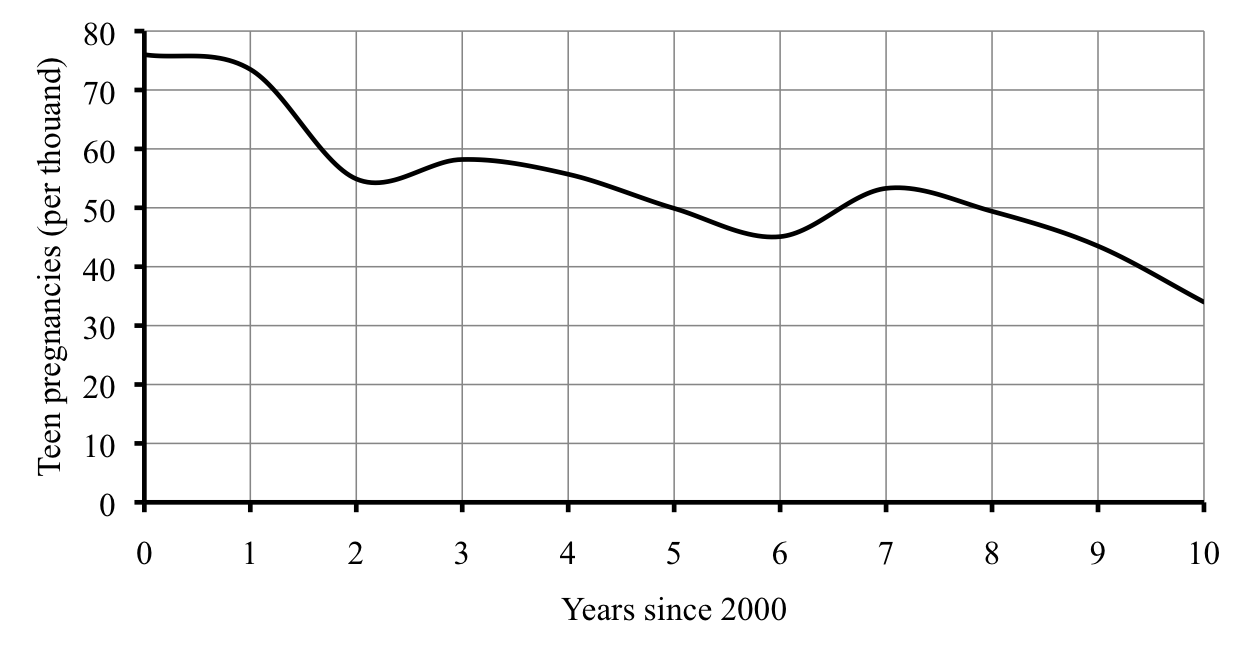
\includegraphics [width = 6in] {teenpregTEST.png}}
%\scalebox {.9} {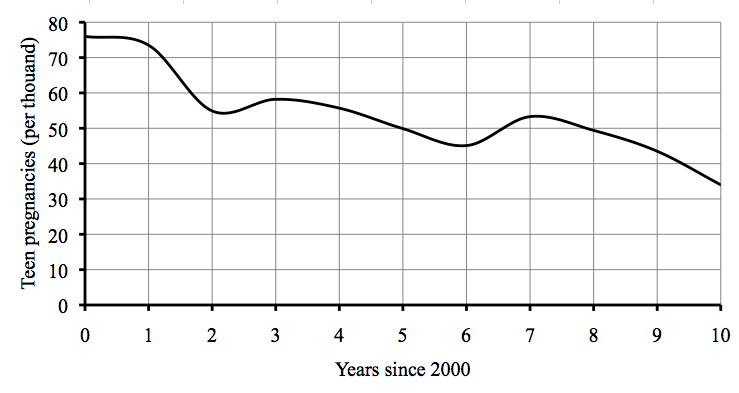
\includegraphics [width = 6in] {teenpreg(fromExcel).png}}
\end{center}
\begin{enumerate}
\item What was the teen pregnancy rate in 2003? \vfill
\item Did the teen pregnancy rate increase or decrease from 2003 to 2004? \vfill
\item While the teen pregnancy rate has generally decreased, from 2002 to 2003 it actually increased.  Were there other times when it increased?  \vfill
\item When did the teen pregnancy rate first fall below 60 pregnancies per thousand teens? \vfill
\item How fast was the teen pregnancy rate dropping on average per year from 2002 to 2005?  How does that compare to 2006 to 2009?   \vfill
\end{enumerate}

\end{enumerate}

 
%	\section{Units  -- Practice exercises}

\begin{enumerate}
\item  
\begin{enumerate}

\item Compare centimeters (cm) and inches, using that 1 inch $\approx$ 2.54 cm
\begin{enumerate}
\item Which is longer:  1 inch or 1 centimeter? \vfill
\item Kamari is shopping at an internationally-based retail store. She's looking at a curtain rod that will project 10 cm from the wall.  What is that in inches?  \vfill
\item She also wants a basket no more than 1 foot wide or long to fit on her bookcase.  How many centimeters are in a foot? \vfill
\end{enumerate}

\item Compare meters (m) and yards using that 1 yard $\approx$ .9144 m
\begin{enumerate}
\item Which is longer: 1 yard or 1 meter? \vfill
\item Princeton was watching the Olympics and noticed everything was measured in meters.  He's curious how long a football field (100 yards) is in meters.  \vfill
\item Kamari found a really big bath towel she likes. It's 1 meter wide and 1.5 meters long.  What are the dimensions in inches?  Use that 1 yard = 3 feet.  \vfill
\end{enumerate}

\item Compare kilometers (km) and miles using that 1 mile $\approx$ 1.609 km
\begin{enumerate}
\item Which is longer:  1 mile or 1 kilometer? \vfill
\item This weekend Princeton and Kamari are doing a 5K run.  How many miles long is that?  Note:  \textbf{5K} is short for 5 kilometers.  \vfill
\item  Princeton is actually in training for a marathon.  How many kilometers is that?  Note: a \textbf{marathon} is approximately 26.2 miles. \vfill
\end{enumerate}

\end{enumerate}

\newpage %%%%%%

\item \begin{enumerate}
\item Yesterday Cameron worked for 2 hours and 15 minutes (that's 2:15) and then went home and studied for 7 hours and 57 minutes (that's 7:57).  Convert each time into decimal hours. \vfill
\item  Ephriam works at a plant that produces very delicate electronic switches.  He measured the lifetime for one switch at 4.18 hours.  Another had lifetime 19.50 hours.  Convert each time into hours and minutes.   \emph{That means H:MM format.}\vfill
\item Phillip measured his office using a digital measure. One wall is 21.8 feet. The other is 10.2 feet.   How long is each wall measured in the more usual feet and inches? \vfill
\item The couch Stetson wanted to buy is 92" long and 44" tall.  Convert the length and height to feet and inches. \vfill
\item Abdi volunteers at a food bank.  He noticed that the shelf on the back wall was bowing so he measured its length at 12'5".  The formula for load needs the length written as a decimal.  Convert the length to a decimal number of feet. \vfill
\end{enumerate}

\newpage %%%%%%

\item Some people say we should drink 8 glasses of water (or other liquids) every day where a glass is defined as 8 (liquid) ounces.
\begin{enumerate}
\item Ingrid uses a 20 ounce unbreakable plastic bottle.  How many of those does she need to drink each day?\vfill
\item Siri carries around a insulated water bottle that holds .6 liters.  How many of those does she need to drink each day?  Use that 1 liter $\approx$ 1.057 quarts and 1 quart = 32 (liquid) ounces.\vfill
\item To meet the recommendation, how much water would one person drink in a year?  Give the answer in gallons.  Use 1 gallon = 4 quarts.\vfill
\end{enumerate}

\newpage %%%%%%

\item Jenna is studying in Finland this term and rented an older car to drive.
\begin{enumerate}
\item Gas prices in Finland were 1.658 \euro/liter.  What's the equivalent price in \$/gal?  Use 1 \euro~$\approx$ \$1.23.  The symbol \euro~stands for euro. \vfill
\item  Her car holds 62 liters of gasoline in its tank.  How many gallons is that?  Use that 1 liter $\approx$ 1.057 quarts and 1 gallon = 4 quarts.\vfill
\item What would it cost, in euros, for a tank full of gas?  In dollars? \vfill
\item Her car gets 7.6 km/liter.  Convert to miles per gallon (mpg).  Use 1 liter $\approx$ 1.057 quarts and 1 gallon = 4 quarts.\vfill
\item Jenna learns that no matter what the road signs might say, the maximum speed limit in Finland in winter is never more than 100 km/hr.  How fast is that in miles per hour (mph)?\vfill
\end{enumerate}

\end{enumerate}

 
%	%!TEX root =  A_WS.tex

\section{Metric prefixes and scientific notation -- Practice exercises}

%\bigskip
%
%Common metric prefixes:
%
%\begin{center}
%\begin{tabular} {lclclcl} 
%\textbf{giga} &$=$& 1 \text{ billion} &$=$& $\text{1,000,000,000}$&$=$&$10^{9}$\\ 
%\textbf{mega} &$=$&1 \text{ million} &$=$&$ \text{1,000,000}$&$=$&$10^{6}$\\
%\textbf{kilo} &$=$&1 \text{ thousand} &$=$&$ \text{1,000}$&$=$&$10^{3}$\\
%\textbf{centi} &$=$&1 in a hundred &$=$&.01&$=$&$10^{-2}$\\
%\textbf{milli} &$=$&1 in a thousand &$=$&.001&$=$&$10^{-3}$\\
%\textbf{micro} &$=$&1 in a million &$=$&.000001&$=$&$10^{-6}$\\
%\textbf{nano} &$=$&1 in a billion &$=$&.000~000~001 &$=$&$10^{-9}$\\
%\end{tabular}
%\end{center}
%
%\newpage

\begin{enumerate}

\item The GDP (gross domestic product) of the United States was approximately \$\text{15,596} billion in 2011 and the population of the United States was approximately 0.313 billion that year.  \hfill \begin{footnotesize} Source:  U.S.\ Bureau of Economic Analysis, U.S.\ Census Bureau\end{footnotesize}
%http://www.tradingeconomics.com/united-states/gdp
%http://www.census.gov/main/www/popclock.html
\begin{enumerate}
\item Writing the population as 0.313 billion seems strange.  A more natural unit would be millions.  Rewrite the population in millions of people. \vfill
\item Rewrite the population in people, both in normal decimal notation (that means with all the 0s) and in scientific notation. \vfill
\item It also seems strange to write the GDP as \$\text{15,596} billion.   A more natural unit would be \textbf{trillions} where
$$1 \text{ trillion} =  \text{ 1,000,000,000,000}$$
Rewrite the GDP in trillions of dollars. \vfill
\item Rewrite the GDP in dollars, both in normal decimal notation and in scientific notation. \vfill
\item Calculate the GDP \textbf{per capita} (meaning per person) by dividing the GDP in dollars by the population in people.  Express your answer in \$/person. \vfill
\item For practice, repeat your calculation using the numbers in scientific notation.  
 
 \emph{Because $\times$ and $\div$ are at the same level in the order of operations, you need to put parentheses around each number in scientific notation before dividing.} \vfill
\end{enumerate}

\newpage %%%%%%

\item Edgar recently changed the cleaning bag on his vacuum cleaner.  He became curious about how many particles of dust were in the bag.  Edgar did a little research online and found out that the mass of a dust particle is .000~000~000~753 kilograms.  

(The strange-looking spaces are to help you see that there are 9 zeros in the number.)
\begin{enumerate}
\item Write the mass of a dust particle in scientific notation. \vfill
\item Recall that 

\begin{center}
\begin{tabular} {lclclcl} 
\textbf{kilo} &$=$&1 \text{ thousand} &$=$&$ \text{1,000}$&$=$&$10^{3}$\\
\textbf{milli} &$=$&1 in a thousand &$=$&.001&$=$&$10^{-3}$\\
\textbf{micro} &$=$&1 in a million &$=$&.000001&$=$&$10^{-6}$\\
\textbf{nano} &$=$&1 in a billion &$=$&.000~000~001 &$=$&$10^{-9}$\\
\end{tabular}
\end{center}

Express the mass of a dust particle in each of the given units.  

\begin{enumerate}
\item  grams \vfill
\item milligrams (mg) \vfill
\item micrograms ($\mu$g)  \vfill
\item nanograms (ng)  \vfill
\end{enumerate}
%% SU you should add this negative exponent description to the section too. Maybe a list of all the prefixes w/ it???
\item Edgar determined that the full vacuum bag weighed 5 pounds. How many dust particles were in the bag?  (I am already sneezing.) Use $1 \text{ kilogram} \approx 2.2 \text{ pounds}$. Express your answer in scientific notation.   \vfill \vfill
\end{enumerate} 

\newpage %%%%%%

\item The list shows the (approximate) mass of the planets in our solar system.
\begin{center}
\begin{tabular} {ll}
Earth & $5.972 \times 10^{24}$ kg \\
Jupiter &  $1.899 \times 10^{27}$ kg  \\
Mars & $6.417 \times 10^{23}$ kg \\ 
Mercury & $3.302 \times 10^{23}$ kg \\
Neptune & $1.024 \times 10^{26}$ kg \\
Saturn & $5.685 \times 10^{26}$ kg \\
Uranus & $8.681 \times 10^{25}$ kg \\
Venus & $4.868 \times 10^{24}$ kg \\ 
\end{tabular}
\end{center}
\hfill \begin{footnotesize} Source:  Wikipedia (Solar System) \end{footnotesize}
% http://en.wikipedia.org/wiki/Solar_System
\begin{enumerate}
\item Write the mass of Earth and the mass of Mars in standard decimal notation.  Which is heavier?\vfill
\item List the planets from heaviest (largest mass) to lightest (smallest mass).\vfill 
\item The mass of astronomical bodies are sometimes measured in \textbf{Jupiter mass} abbreviated $M_J$ where $1 M_J = 1.899 \times 10^{27}$ kg.  Express Earth's mass in $M_J$.

 \emph{Because $\times$ and $\div$ are at the same level in the order of operations, you need to put parentheses around each number in scientific notation before dividing.} \vfill
\end{enumerate}

\newpage %%%%%%

\item Souksavanh is setting up a patient's intravenous (IV) medication. She sets the drip at 42 drops/minute.  The drip chamber size is 20 drops/mL.  Recall

\begin{center}
\begin{tabular} {lclclcl} 
\textbf{milli} &$=$&1 in a thousand &$=$&.001&$=$&$10^{-3}$\\
\textbf{micro} &$=$&1 in a million &$=$&.000001&$=$&$10^{-6}$\\
\end{tabular}
\end{center}
\begin{enumerate}
%\item Souk needs to know a few conversions.
%\begin{enumerate}
%\item How many milliliters (mL) are in a liter? \bigskip
%\item How many microliters ($\mu$L) are in a liter? \bigskip
%\item How many milligrams (mg) are in a gram? \bigskip
%\end{enumerate}
%\hspace{-.35in}  Use these numbers to answer the following questions. %HSPACE
\item At what rate is the IV fluid being delivered to Souk's patient?  Answer in mL/min (millileters per minute). \vfill
\item How fast is the drip measured in $\mu$L/sec (microliters per second)? \vfill
\item If the drip bag holds 1 liter, how long will it take the drip to run?  Express your answer in hours and minutes.\vfill
\item The concentration of medication is 1.7 mg/mL (milligrams per milliliter).  How much medication is in the 1 liter bag?  Convert your answer to grams.  Explain what you notice.\vfill
\item At what rate is the medication being delivered to Souk's patient?  Answer in g/min (grams per minute).\vfill
\end{enumerate}

\end{enumerate} 

\newpage


\noindent \textbf{When you're done \ldots}

\begin{itemize}
\item [$\Box$] Check your solutions.  Still confused?  Work with a classmate, instructor, or tutor.
\item [$\Box$] Try the \textbf{Do you know} questions.  Not sure?  Read the textbook and try again.
\item [$\Box$] Make a list of key ideas and process to remember under \textbf{Don't forget!}
\item [$\Box$] Do the textbook exercises and check your answers. Not sure if you are close enough? Compare answers with a classmate or ask your instructor or tutor.  
\item [$\Box$] Getting the wrong answers or stuck?  Re-read the section and try again.   If you are still stuck, work with a classmate or go to your instructor's office hours or tutor hours.
\item [$\Box$] It is normal to find some parts of exercises difficult, but if most of them are a struggle, meet with your instructor or advisor about possible strategies or support services.
\end{itemize}





%\bigskip

\noindent \textbf{Do you know \ldots} % Metric system and scientific notation

\begin{enumerate} [(a)]
\item How to calculate powers on your calculator?
\item What  million, billion, and trillion mean?  
\item Why metric prefixes are used?  
\item What common metric prefixes (mega, giga, kilo, centi, milli, micro, nano) mean? 

\emph{Ask your instructor which prefixes you need to remember, and whether any prefixes will be provided during the exam.} 
\item Why scientific notation is used?  
\item The standard format for scientific notation?  
\item What kinds of numbers have a positive order of magnitude, and which have a negative order of magnitude?
\item How to convert between decimal notation and scientific notation?  
\item How your calculator reports numbers in scientific notation, and what (might be) different when you're reporting that number?  
%\item How to enter numbers written in scientific notation into your calculator? 
\item The usual order of operations (PEMDAS) and how to use parentheses when you want a different order?
\end{enumerate}

\bigskip

\noindent \textbf{Don't forget!}


 
%	%!TEX root =  A_WS.tex

\section*{Practice Exam 1A}  
\markright{Practice Exam 1A}
\addcontentsline{toc}{section}{Practice Exam 1A}

Relax.  You have done problems like these before.  Even if these problems look a bit different, just do what you can.  If you're not sure of something, please ask! You may use your calculator.  Please show all of your work and write down as many steps as you can.  Don't spend too much time on any one problem.  Do well.  And remember, ask me if you're not sure about something. \bigskip

\noindent \emph{As you work, make a ``don't forget'' list of any information you need to look up or ask about.} 

\noindent \hrulefill
\bigskip

\begin{enumerate}
 
 \item Arva and Ellie began hiking at an elevation of 1,500 feet and climbed at the steady rate of 600 vertical feet per hour. 
\begin{enumerate}
\item Make a table showing their elevation after 1 hour, 2 hours, and 5 hours. \vfill \vfill
\item Name the variables, including units. \vfill \vfill
\item Explain the dependence using a sentence of the form ``\underline{~\quad} is a function of \underline{~\quad}.'' \vfill
\item Is the function increasing or decreasing? \vfill
\item How long does it take them to reach 5,300 feet up?  Try to figure out the answer in hours and minutes (H:MM format). \vfill \vfill \vfill
\end{enumerate}

\newpage

\item The table shows Henry's weight as a baby.
\begin{center}
\begin{tabular} {|l||c|c|c|} \hline
Age (weeks) & 0 & 12 & 15 \\ \hline
Weight (pounds) & 8 & 14 & 16 \\ \hline
\end{tabular}
\end{center}
\begin{enumerate}
\item How much weight did Henry gain, on average, each week during his first 12 weeks? \vfill
\item During which time interval was Henry gaining weight faster?  \emph{Explain.} \vfill
 \item Identify the variables, including units and dependence. \vfill
 \item Draw a graph illustrating the dependence.  Choose a scale that shows up to 20 weeks and 20 pounds. \bigskip
\begin{center}
\scalebox {.8} {
\includegraphics [width = 6in] {GraphPaper.jpg}}
\end{center}

\bigskip
\item What might you guess for Henry's weight at 20 weeks?   \vfill
\end{enumerate} 

\newpage

\item Pramesh's new car used 20.5 gallons of gas for a 715 mile trip. 
\begin{enumerate}
\item How many miles per gallon (mpg) does his car get? \vfill
\item At that rate, how many gallons of gas would Pramesh use on his 3,200 mile cross-country trip?  \vfill
\item If gas costs \$3.799/gallon, how much will gas for that trip cost?  \vfill
\end{enumerate}

\newpage

\item Ndwiga is reading an article in the paper about atoms.  From his physics textbook he discovered that the size of an atom is .142 nanometers.  (That's 0.142 nanometers.)
\begin{enumerate}
\item Write the size of an atom in meters.  Use $1 \text{ meter} = \text{1,000,000,000 nanometers}$.   Write your answer in usual decimal notation and in scientific notation. \vfill \vfill
\item Ndwiga would like to know how many atoms across this sheet of paper which is 8.5 inches wide. Use that $1 \text{ inch} \approx 2.54 \text{ cm}$ and $1 \text{ meter} = 100 \text{ cm}$.  Express your final answer in billions of atoms. \vfill \vfill \vfill
\end{enumerate}

%%%% END

\end{enumerate}


%	%!TEX root =  A_WS.tex

\section*{Practice Exam 1B}  
\markright{Practice Exam 1B}
\addcontentsline{toc}{section}{Practice Exam 1B}

\emph{Try taking this version of the practice exam under testing conditions:  no book, no notes, no classmate's help, no electronics (computer, cell phone, television). Give yourself one hour to work and wait until you have tried your best on all of the problems before checking any answers.}

\noindent \hrulefill

\begin{enumerate}

\item The amount of money spent on nursing home care for seniors has continued to rise.  The table shows the values for select years.  Here $S$ is the spending, measured in billions of dollars and $Y$ is the year, measured in years since 1960.

\begin{center}
\begin{tabular} {|c ||c |c |c |c |c |c |c |} \hline
$Y$ & 0 & 10 & 25 & 40 & 52 \\ \hline
$S$ & 1.0 & 3.3 & 33.7 & 96.6 & 170.3 \\ \hline
\end{tabular}
\end{center}

\begin{enumerate}
\item According to the table, what was the spending in 1970?  \vfill
\item According to the table, what was the spending in 1985?  \vfill
\item Calculate the rate of change of spending over the period 1970 to 1985.  Don't forget to state the units. \vfill \vfill
\item In approximately what year did spending first pass \$50 billion? \vfill
\end{enumerate}

\newpage

\item Trish is filling a swimming pool with water.  The graph below shows how many gallons of water ($G$) are in the pool after $H$ hours.  Use the graph to answer the following questions.
\begin{center}
\scalebox {.9} {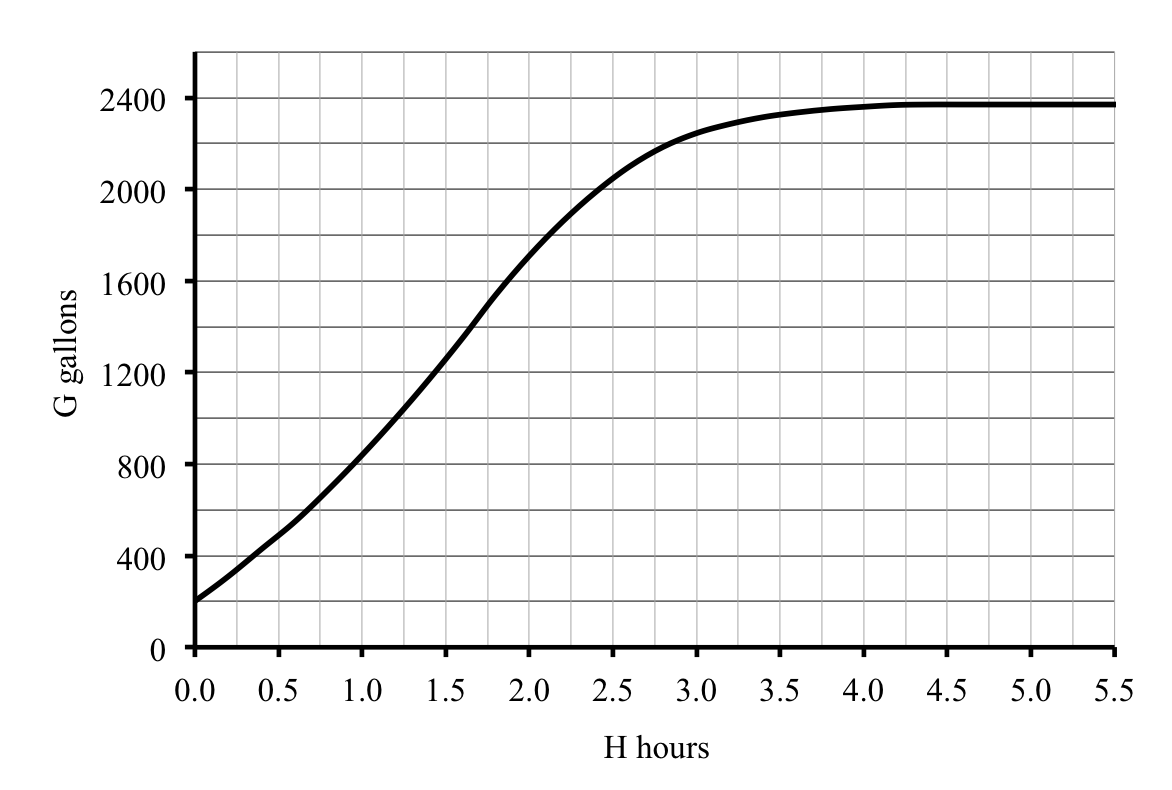
\includegraphics [width = 6in] {fillingtankNEW}}
\end{center} 
\begin{enumerate}
\item How much water was in the swimming pool already when Trish began? \vfill
\item How much water was in the swimming pool after 3 hours? \vfill
\item After how many hours were there 1,000 gallons of water in the swimming pool? \vfill
\item Was Trish filling the pool faster at 2 hours or at 2.5 hours?  Explain how you see that on the graph. \vfill
\item After (about) how many hours did Trish stop filling the swimming pool?  Explain how you see that on the graph. \vfill
\end{enumerate}

\newpage

\item In 1990 the Lef\`evre's property tax was \$450 but it doubled every year thereafter.  
 \begin{enumerate}
 \item Name the variables, including units. \vfill \vfill
 \item Which is the independent variable and which is the dependent variable? \vfill
\item Make a table showing the property tax each year from 1990 to 1994. \vfill \vfill
\item Draw a graph illustrating the dependence.
\bigskip
\begin{center}  
\scalebox {.8} {
\includegraphics [width = 6in] {GraphPaper.jpg}}
\end{center}
\bigskip
 \end{enumerate} 
 
\newpage

\item The distance from the Earth to the Moon is approximately 384,000,000 meters. 

\hfill \begin{footnotesize} Source:  Wikipedia (Lunar distance)\end{footnotesize}
\begin{enumerate}
\item Express this distance in scientific notation. \vfill
\item Express this distance in kilometers (km), using $1 \text{ km} = \text{1,000 meters}$. \vfill \vfill
\item Express this distance in miles, using the conversion $1 \text{ mile} \approx 1.609 \text{ km}$. \vfill \vfill
\item If you could drive to the moon at 55 mph, how long would it take to get there? Express your answer in terms of months, using $1 \text{ month} \approx 30 \text{ days}$. \vfill \vfill \vfill
\end{enumerate}

%%%% END

\end{enumerate}


%            
%\chapter{Equations}


%     % %!TEX root =  A_WS.tex

\section*{Formulas for Chapter 2}  
\markright{Formulas for Chapter 2}
\addcontentsline{toc}{section}{Formulas for Chapter 2}

 \bigskip
 \bigskip
\noindent \hrulefill
 \bigskip
 \bigskip

 \noindent \textsc{Percent Change Formula:} \quad
 If a quantity increases by a percentage corresponding to growth rate $r$, then the growth factor is $$\displaystyle g=1+r$$ 
 
\noindent \hrulefill
 \bigskip
 \bigskip

\noindent \textsc{Compound Interest Formula:} \quad
$\displaystyle a = p \left( 1 + \frac{r}{12}\right) ^{12y}$ 

\bigskip
\bigskip

\noindent \textsc{Equivalent APR Formula:} \quad 
$\displaystyle \text{APR} = \left(1+\frac{r}{12}\right)^{12}-1$ 

\bigskip
\bigskip

\noindent  \textsc{Future Value Annuity Formula:} \quad
$\displaystyle a = p \ast \frac{\left( 1 + \frac{r}{12}\right) ^{12y}-1}{\frac{r}{12}}$ 

\bigskip
\bigskip

\noindent  \textsc{Loan Payment Formula:} \quad
$\displaystyle p = \frac{a  \ast \frac{r}{12}}{1-\left( 1 + \frac{r}{12}\right) ^{-12y}}$ 

\bigskip
\bigskip

\noindent  where 
\begin{center}
\begin{tabular} {l} 

$a$ = account balance or loan amount (\$) \\
$p$ = initial deposit (principal), regular deposit, or regular payment (\$) \\
$y$ = time invested (years)\\
$r$ = interest rate compounded monthly (as a decimal) \\ 
\end{tabular}
\end{center}

 \bigskip
 \bigskip
\noindent \hrulefill
 \bigskip
 \bigskip

\vfill %VFILL
%      \section{A first look at linear equations -- Practice exercises}

\begin{enumerate}

\item A truck hauling bags of grass seed pulls into a weigh station along the highway.  Trucks are weighed to determine the amount of highway tax.  This particular truck weighs \text{3,900} pounds when it's empty.  Each bag of seed it carries weighs 4.2 pounds. 
For example, a truck is carrying \text{1,000} bags of grass seed weighs 
$$\text{3,900 pounds } + \frac{4.2 \text{ pounds}}{\text{bag}} \ast \text{1,000  bags} = \text{3,900} + 4.2\times\text{1,000}=\text{8,100 pounds}$$ 
In official trucking lingo, we  say the \textbf{curb weight} of \text{3,900} pounds plus the \textbf{load weight} of \text{4,200} pounds results in a \textbf{gross weight} of \text{8,100} pounds.  So, now you know.  \hfill \emph{Story also appears in 3.1\#1 and 3.2 \#1}
\begin{enumerate}
\item Calculate the gross weight of the truck if it contains \text{2,000} bags of grass seed.   \vfill
\item Name the variables, including units, and  write an equation showing how the gross weight of the truck is a function of the number of bag seed it contains.  \vfill
\item Identify the slope and intercept, along with their units, and explain what each means in terms of the story. \vfill
\item The bags of grass seed are piled on wood \textbf{pallets} (a sturdy platform) to make them more stable for moving. How much does the truck weigh if it is carrying 12 pallets of grass seed bags, where each pallet holds 96 bags of seed?    \vfill
\end{enumerate}

\newpage %%%%%%

\item The water in the local reservoir was 47 feet deep but there's been so little rain that the depth has fallen 18 inches a week over the past few months.  Officials are worried if dry conditions continue the reservoir will not have enough water to supply the town.  

\hfill \emph{Story also appears in 3.2 Exercises and 4.1 \#3}
\begin{enumerate}
\item Name the variables and write an equation relating them.  First convert 18 inches to feet. \vfill
\item Identify the slope and intercept, along with their units, and explain what each means in terms of the story. \vfill
\item Make a table of values showing the projected depth of the reservoir after 1 week, 5 weeks, 10 weeks, and 20 weeks if the current trend continues. \vfill
\item Draw a graph illustrating the function.
\begin{center}
\scalebox {.8} {
\includegraphics [width = 6in] {GraphPaper.jpg}}
\end{center}
\end{enumerate}

\newpage %%%%%%

\item   I was short on cash so I got a  \textbf{line of credit} (short term loan) on my bank account, of which I spent \$\text{2,189.57}. That means my account balance is $-$\$\text{2,189.57}.  I will pay back the interest plus an extra \$250 each month.  When the loan is paid off,  I plan to continue to deposit \$250 per month to start saving. 
 
  \hfill \emph{Story also appears in 3.2 Exercises}
\begin{enumerate}
\item Name the variables and write an equation relating them.  Ignore the interest. \vfill
\item Identify the slope and intercept, along with their units, and explain what each means in terms of the story.  \vfill
\item Make a table of values showing the projected account balance now, after 4 months, and at the end of a year.    \vfill \vfill
\item Draw a graph showing how my account balance changed in a year's time.
\begin{center}
\scalebox {.8} {
\includegraphics [width = 6in] {GraphPaper.jpg}}
\end{center}
\bigskip
\item About how many months will it take to pay off my line of credit?   \bigskip
\end{enumerate} 

\newpage %%%%%%

\item  A mug of coffee costs \$3.45 at Juan's favorite cafe, unless he buys their discount card for \$10 in which case a mug costs  \$2.90.
    \hfill \emph{Story also appears in 1.2 \#4 and 4.2 \#2}
\begin{enumerate}
\item Name the variables, including units. \vfill
\item Write an equation describing how the total cost depends on how many mugs of coffee Juan buys without the discount card. \vfill
\item Write an equation describing how the total cost depends on how many mugs of coffee Juan buys if he does buy the discount card. \vfill
\item How would the equation change if the cafe offer a new annual membership card that cost \$59.99 but entitles Juan to buy coffee for only \$1 per cup all year? \vfill
\end{enumerate} 

\end{enumerate} 
%      %!TEX root =  A_WS.tex

\section{A first look at exponential equations  -- Practice exercises}

\begin{enumerate}  

 \item The comprehensive fee at a local private college is \$37,000.  The fee is projected to increase 5.8\% per year.
\begin{enumerate}
\item Calculate the annual growth factor. \vfill
 \item What do you expect the comprehensive fee will be in five years? \vfill
\item Name the variables, including units, and write an equation describing the dependence. \vfill
\item Make a table of values showing the comprehensive fee now, in 5 years, 10 years, 20 years, and 50 years (even though that's not realistic).  \vfill
\item Draw a graph illustrating the function.
\begin{center}
\scalebox {.8} {
\includegraphics [width = 6in] {GraphPaper.jpg}}
\end{center}
\end{enumerate}

\newpage %%%%%%

\item Bunnies, bunnies, everywhere.  They eat the tops of my tulips in early spring and my lilies all summer long.  Back in 2007 there were an estimated  1,800 rabbits in my neighborhood. Rabbits multiply quickly, 13\% per year by one estimate.  

\hfill \emph{Story also appears in 5.1\#3}
\begin{enumerate}
\item Name the variables, including dependency. \vfill
\item Calculate the annual growth factor. \vfill
\item What does this story suggest the rabbit population was in 2010?  In 2013? \vfill
\item Write an equation relating the variables. \vfill
\end{enumerate}  

\newpage %%%%%%

\item A flu virus has been spreading through the college dormitories. Initially 8 students were diagnosed with the flu, but that number has been growing  16\% per day.   

\hfill \emph{Story also appears in  5.1 \#2 and 5.5 textbook}
\begin{enumerate}
\item Calculate the daily growth factor and use it to write an equation describing the spread of the virus.  Don't forget to name the variables too.  \vfill  \vfill
\item Make a table and graph for the six weeks following the initial diagnosis.  (That means use 0, 7, 14, 21, 28, 35, and 42 days.)  \vfill  \vfill
\begin{center}
\scalebox {.8} {
\includegraphics [width = 6in] {GraphPaper.jpg}}
\end{center}
\bigskip
\item What is a realistic domain?  That means, for how many days do you think this model is reasonable? To keep a sense of scale, there are 1,094 students currently living in the dorms. \vfill
\end{enumerate}  

\newpage %%%%%%

\item My savings account earns a modest amount of interest, the equivalent of .75\% annually.  I have \$12,392.18 in the account now.  
\begin{enumerate}
\item How much interest will I earn this year? \vfill
\item What will my balance be in three years, assuming I neither deposit nor withdraw money? \vfill
\item Name the variables and write an equation relating them. \vfill
\item What would the equation be if I moved all of my money into a certificate of deposit earning the equivalent of .92\%? \vfill
\item What would the equation be if I moved \$10,000 into that certificate of deposit, and kept the rest in savings? 
\emph{Hint:  to find the total balance, add the amounts.} \vfill
\end{enumerate}

\end{enumerate} 

\newpage


\noindent \textbf{When you're done \ldots}

\begin{itemize}
\item [$\Box$] Check your solutions.  Still confused?  Work with a classmate, instructor, or tutor.
\item [$\Box$] Try the \textbf{Do you know} questions.  Not sure?  Read the textbook and try again.
\item [$\Box$] Make a list of key ideas and process to remember under \textbf{Don't forget!}
\item [$\Box$] Do the textbook exercises and check your answers. Not sure if you are close enough? Compare answers with a classmate or ask your instructor or tutor.  
\item [$\Box$] Getting the wrong answers or stuck?  Re-read the section and try again.   If you are still stuck, work with a classmate or go to your instructor's office hours or tutor hours.
\item [$\Box$] It is normal to find some parts of exercises difficult, but if most of them are a struggle, meet with your instructor or advisor about possible strategies or support services.
\end{itemize}





\bigskip

\noindent \textbf{Do you know \ldots} %First_look_exponential

\begin{enumerate} [(a)]
\item How to find the growth factor if you know the percent increase?    
\item How to calculate percent increase in one step?   
\item What makes a function exponential?   
\item The template for an exponential equation? \emph{Ask your instructor if you need to remember the template or if it will be provided during the exam.} 
\item Where the starting value and growth factor appear in the template for an exponential equation?   
\item What the graph of an exponential function looks like? 
\end{enumerate}

\bigskip

\noindent \textbf{Don't forget!}

 
%      %!TEX root =  A_WS.tex

\section{Using equations  -- Practice exercises} 

\begin{enumerate}

\item Dontrell and Kim borrowed money to buy a house on a 30-year mortgage.  
%At today's favorable interest rates, they pay  \$944 a month. (Plus taxes and insurance.)  
After $M$ months of making payments, Dontrell and Kim will still owe \$$D$ where 
$$D=236,000-56,000 \ast 1.004^M$$  
$D$ is also known as the \textbf{payoff} (how much they would need to pay to settle the debt).
% Based on $j_{12}=4.8\%$

 \hfill \emph{Story also appears in 3.4 \#4}
 \begin{enumerate}
\item How much did Dontrell and Kim originally borrow to buy their house?  What value of $M$ did you evaluate at to answer the question? \vfill
\item Evaluate the equation at $M=12$ and explain what the answer means in terms of the story. \vfill
\item After making half the payments, how much money will Dontrell and Kim still owe on the house?  Will they have paid more or less (or exactly) half of the loan?  \emph{Hint:  convert 30 years into months to find the total number of payments.  Then divide by 2 to find the halfway point.} \vfill
\item The very last month they do not actually pay the regular monthly payment, just whatever balance is left on the loan.  How much will that be? \emph{Hint:  they will have made all but one of the payments.} \vfill
\end{enumerate}

\newpage %%%%%%

\item ``Rose gold'' is a mix of gold and copper.  We start with 2 grams of an alloy that is equal parts gold and copper and add $A$ grams of pure gold to lighten the color. The percentage of gold in the resulting rose gold alloy, $R$ is given by $$R = 100\left(\frac{1+A}{2+A}\right)$$
For example, if we add 0.8 grams of pure gold, then $A=.8$ and so the percentage is $$R=100\left(\frac{1+.8}{2+.8}\right)= 100 \times (1 + \underline{.8})\div(2+\underline{.8})=64.28571428\ldots \approx 64.3\%$$ 

\vspace{-.15in} %VSPACE
\hfill \emph{Story also appears in 4.1 Exercises}

\begin{enumerate}
\item Calculate the percentage of gold in the alloy if we add 1.2 grams of pure gold. \vfill \vfill
\item Fill in that and the rest of the missing values.
\begin{center}
\begin{tabular} {|c| |c |c |c |c |c |c |c  |c|}\hline
$A$ & 0 &  .4 & .8 & 1.2  & 1.6  & 2 & 3 & 4 \\  \hline
&&&&&&&& \\ 
$R$ &50.0 & \hspace{.5 in}~& 64.3 & \hspace{.5 in}~  & 72.2 & \hspace{.5 in}~& 80.0 &\hspace{.5 in}~\\
&&&&&&&& \\ \hline
\end{tabular}
\end{center}
\item Graph the function.
\begin{center}
\scalebox {.8} {
\includegraphics [width = 6in] {GraphPaper.jpg}}
\end{center}
\bigskip
\item What do you think happens to the percentage of gold as we add more and more pure gold?  Try adding 10 grams, and then try adding 100 grams to check. \vfill
\end{enumerate}

\newpage %%%%%%

\item Monty hopes to grow orchids but they are fragile plants.  He will consider his greenhouse a success if at least nine of the ten orchids survive.  Assuming the orchids each survive at rate $S$, the probability his greenhouse is a success, $P$, is given by 

\begin{tabular} {ccr}
\hspace{1.55in} &$P= 10S^9-9S^{10}$ \hspace{.5in}~& \emph{Story also appears in 2.4 \#3}  \\
\end{tabular}
\begin{enumerate}
\item If the orchids are perfect ($S=1$), what is the probability of a successful greenhouse?  Explain how this answer makes sense in the story. \vfill
\item If the orchids are complete duds ($S=0$), what is the probability of a successful greenhouse?  Explain how this answer makes sense in the story. \vfill
\item Make a table comparing the probability of a successful greenhouse if the orchids each survive at rate $S = 0, .5, .8, .9, .95, $ or $1$. \vfill \vfill
\item Draw a graph of the function.
\begin{center}
\scalebox {.8} {
\includegraphics [width = 6in] {GraphPaper.jpg}}
\end{center}
\end{enumerate}

\newpage %%%%%%

\item Valerie plans to do a 3-day, 50-mile walk to raise money for breast cancer research, in honor of her aunt.  Valerie's friends have pledged a total of  \$93 per mile.   
\begin{enumerate}
\item Valerie hopes to walk all 50 miles.  If so, how much money will she raise? \vfill
\item She might have to stop sooner, however. Name variables and write an equation showing how the money Valerie raises is a function of how far she is able to walk.  \vfill \vfill
\item How long will it take Valerie to walk the full 50 miles if she is able to keep a pace of 3.2 miles per hour? Write your answer in H:MM format. \vfill \vfill
\item Name the new variables and write a new equation showing how the time it takes Valerie to walk the full 50 miles depends on her pace.  \vfill \vfill
\item Good news.  Valerie walked the full 50 miles at a pace of 3.2 miles per hour.  Way to go, girl!   How much money did she raise each hour? 

 \emph{Hint: use your answers from (a) and (c) to get \$/hour.}  \vfill
\end{enumerate}

\end{enumerate}

\newpage


\noindent \textbf{When you're done \ldots}

\begin{itemize}
\item [$\Box$] Check your solutions.  Still confused?  Work with a classmate, instructor, or tutor.
\item [$\Box$] Try the \textbf{Do you know} questions.  Not sure?  Read the textbook and try again.
\item [$\Box$] Make a list of key ideas and process to remember under \textbf{Don't forget!}
\item [$\Box$] Do the textbook exercises and check your answers. Not sure if you are close enough? Compare answers with a classmate or ask your instructor or tutor.  
\item [$\Box$] Getting the wrong answers or stuck?  Re-read the section and try again.   If you are still stuck, work with a classmate or go to your instructor's office hours or tutor hours.
\item [$\Box$] It is normal to find some parts of exercises difficult, but if most of them are a struggle, meet with your instructor or advisor about possible strategies or support services.
\end{itemize}





\bigskip

\noindent \textbf{Do you know \ldots} % Using equations

\begin{enumerate} [(a)]
\item What it means to �evaluate� a function? 
\item Why some numbers are underlined in our calculation?
\item How to evaluate an function when the independent variable occurs more than once? 
\item How to generate a table or graph from an equation? 
\item What graphs of different types of functions look like? 
\item What a power, polynomial, or quadratic equation look like?
\end{enumerate}

\bigskip

\noindent \textbf{Don't forget!}


 
%      \section{Approximating solutions of equations -- Practice exercises}

\begin{enumerate}

\item The size of a round pizza is described by its \textbf{diameter} (distance across).  Assuming a 16-inch diameter pizza serves four people, and with a little geometry to help us out, we calculated that a pizza of diameter $D$ inches serves $P$ people where 

\begin{tabular} {ccr}
\hspace{.9in} &$P = .015625D^2$ \hspace{.5in}~& \emph{Story also appears in 3.3 \#1 and 4.1 \#3}  \\
\end{tabular}

\begin{enumerate}
\item Confirm that a 16-inch pizza serves four people. \vfill
\item How many people does a 12-inch pizza serve?  A 14-inch pizza? \vfill
\item Graph the function.  Include what happens when $D=0$.
\begin{center}
\scalebox {.8} {
\includegraphics [width = 6in] {GraphPaper.jpg}}
\end{center}
\bigskip
\item A \textbf{personal} pizza is sized to serve one person. Use successive approximation to estimate the diameter of a personal pizza to the nearest inch.  \vfill \vfill
\item What diamter should an extra large pizza be to serve 6 people?  Answer to the nearest \nicefrac{1}{10} inch.  \vfill \vfill
\end{enumerate} 

\newpage %%%%%%

\item Suppose a car gas tank is designed to hold enough fuel to drive 350 miles. (That's fairly average.)  A hybrid car with fuel efficiency of 50 miles per gallon (mpg) would only need a 7 gallon gas tank, but a recreational vehicle that gets only 10 mpg would need a 35 gallon gas tank.    \hfill \emph{Story also appears in 3.3 \#3}
\begin{enumerate}
\item Name the variables including units.  The way the story is stated, the size tank is a function of the fuel efficiency. \vfill
\item Write an equation describing this function. \vfill
\item My Honda Accord's tank holds about 16 gallons.  Approximate the corresponding fuel efficiency to one decimal place.  \vfill
\item My ex-husband's Honda Civic's tank holds only 13 gallons.  Approximate the corresponding fuel efficiency to one decimal place.  \vfill
\item Draw a graph showing how the size tank depends on the fuel efficiency
\begin{center}
\scalebox {.8} {
\includegraphics [width = 6in] {GraphPaper.jpg}}
\end{center}
\end{enumerate} 

\newpage %%%%%%

\item Monty hopes to grow orchids but they are fragile plants.  He will consider his greenhouse a success if at least nine of the ten orchids survive.  Assuming each orchid survives independently with probability $P$, the probability his greenhouse is a success, $G$, is given by 

\begin{tabular} {ccr}
\hspace{1.55in} &$G= 10P^9-9P^{10}$ \hspace{.5in}~& \emph{Story also appears in 2.3 \#1}  \\
\end{tabular}

\begin{enumerate}
\item Monty can buy orchids guaranteed to have a probability .8 of survival each.  Is that enough to give probability .8 of a successful greenhouse?  \vfill
\item What quality of orchids would Monty need to have probability .8 of a successful greenhouse?  \emph{Answer to two decimal places.} \vfill \vfill
\item What quality of orchids would Monty need to have probability .95 of a successful greenhouse?  \emph{Answer to three decimal places.} \vfill \vfill
\end{enumerate}  

\newpage %%%%%%

\item After China, India, and the United States, the next five most populous countries (in 2011) are Indonesia, Brazil, Pakistan, Nigeria, and Bangladesh.  Their projected growth rates and corresponding equation are listed below.  Here $Q$ is the population measured in millions  and $Y$ is the years since 2011. \hfill \begin{footnotesize} Source:  CIA Factbook \end{footnotesize}
\vspace{-.25in} %VSPACE

\begin{center}
\begin{tabular} {lllll}
$4^{\text{th}}$ & Indonesia \quad ~& pop. 248 million \quad ~& growth rate 1.04\% \quad ~& $Q= 248 \ast 1.0104^Y$\\
$5^{\text{th}}$ & Brazil & pop. 205 million & growth rate 1.10\%& $Q = 205  \ast 1.0110^Y$\\
$6^{\text{th}}$ & Pakistan & pop. 190  million & growth rate 1.55\% & $Q = 190 \ast 1.0155^Y$\\
$7^{\text{th}}$& Nigeria & pop. 170  million & growth rate 2.55\% & $Q = 170 \ast 1.0255^Y$\\
$8^{\text{th}}$ & Bangladesh & pop. 161  million & growth rate 1.58\% & $Q = 161\ast 1.0158^Y$\\
\end{tabular}
\end{center}
\begin{enumerate}
\item Which of these countries is projected to have the largest population in 2020?  In 2030?  In 2050? \vfill
\item Explain why Bangladesh's population will not overtake Nigeria's, assuming these projections are accurate. \vfill
\item Approximately when will Brazil's population top 500 million?  Will Nigeria get there first?  Display your work in a table. \vfill
\end{enumerate}

\end{enumerate}

 
%      %!TEX root =  A_WS.tex

\section{Finance formulas  -- Practice exercises}

 \bigskip
 
\noindent \hrulefill

 \bigskip

\noindent \textsc{Compound Interest Formula:} \quad
$\displaystyle a = p \left( 1 + \frac{r}{12}\right) ^{12y}$ 

\bigskip

\noindent \textsc{Equivalent APR Formula:} \quad 
$\displaystyle \text{APR} = \left(1+\frac{r}{12}\right)^{12}-1$ 

\bigskip

\noindent  \textsc{Future Value Annuity Formula:} \quad
$\displaystyle a = p \ast \frac{\left( 1 + \frac{r}{12}\right) ^{12y}-1}{\frac{r}{12}}$ 

\bigskip

\noindent  \textsc{Loan Payment Formula:} \quad
$\displaystyle p = \frac{a  \ast \frac{r}{12}}{1-\left( 1 + \frac{r}{12}\right) ^{-12y}}$ 

\bigskip

\noindent  where 
\begin{center}
\begin{tabular} {l} 

$a$ = account balance or loan amount (\$) \\
$p$ = initial deposit (principal), regular deposit, or regular payment (\$) \\
$y$ = time invested (years)\\
$r$ = interest rate compounded monthly (as a decimal) \\ 
\end{tabular}
\end{center}

\noindent \hrulefill
\newpage %%%%%%

\begin{enumerate}
\item Use the indicated formulas to help Kiran figure out her finances.
%\item (a) \$3,305.13 \quad (b) 7.23\% \quad (c) \$415,475 \quad (d) \$400.65
\begin{enumerate}
\item Kiran deposited \$\text{2,500} in a money market account that earned 7\% interest compounded monthly.  Use the \textsc{Compound Interest Formula} to calculate her account balance after 4 years. \vfill
\item What is the equivalent APR on Kiran's money market account?  Use the \textsc{Equivalent APR Formula.} \vfill
\item Kiran puts \$400 a month in her retirement account that amazingly also earns 7\% interest compounded monthly.  Use the \textsc{Future Value Annuity Formula} to determine how much Kiran will have in her retirement account in 28 years. \vfill
\item Kiran would really like to buy a new hybrid car that sells for \$\text{23,500}.  Sadly Kiran's credit rating is not very good, so the best the dealership offers is a loan at (you guessed it) 7\% interest compouned monthly.  Use the \textsc{Loan Payment Formula} to calculate her monthly car payments on a six year loan. \vfill
\end{enumerate}

\newpage %%%%%%

\item Tim and Josh are saving for their kids' college in fifteen years. The account pays the equivalent of 5.4\% interest compounded monthly (taking into consideration various tax incentives). 
 \begin{enumerate}
\item Make a table comparing how much they will have after fifteen years if  they contribute  \$100 per month vs.\ \$500 per month vs.\ \$\text{1,000} per month. Use the \textsc{Future Value Annuity Formula}. \vfill  \vfill \vfill
\item Tim's parents decide to put \$\text{15,000} into the account now.  How much will that deposit be worth in fifteen years?  Use the \textsc{Compound Interest Formula}.  \vfill  \vfill
\end{enumerate}
%\item 
%\begin{tabular} {|c |c |c |c|}\hline
%$P$ & 100 & 500 & 1000 \\ \hline
%$A$ & 27,640.60 & 138,203.01 & 276,406.03 \\ \hline
%\end{tabular}

\item Use the \textsc{Equivalent APR Formula} to find the APR for each of the following published interest rates (compounded monthly) offered by recent credit card companies.
%\item (a) 9.38\% \quad (b) 12.58\% \quad (c) 22.17\%
\begin{enumerate}
\item 9\% \vfill
\item 12.8\%   \vfill
\item 20.19\% \vfill
\end{enumerate}

\newpage %%%%%%

\item  Cesar and Eliana are looking at three different houses to buy.  The first is a large new townhouse priced at \$\text{240,000}.  The second is a small but charming bungalow priced at \$\text{260,000}.  The third is a large 2-story house down the block priced at \$\text{280,000}. 
%\item (a) 
%\begin{tabular} {|c |c |c |c|}\hline
%$A$ & 240,000 & 260,000 & 280,000  \\ \hline
%$P$ & 1,077.71 & 1,167.52 & 1,257.33 \\ \hline
%\end{tabular}
%\quad (b) Increases monthly payment by \$89.81
 \begin{enumerate}
\item Calculate the monthly payment for each house for a 30-year mortgage at 3.5\% interest compounded monthly.   Use the \textsc{Loan Payment Formula}. 
\bigskip

Townhouse \vfill

Bungalow \vfill

2-Story \vfill

\item Describe the effect on Cesar and Eliana's monthly payment of each \$\text{20,000} increase in the house price  at this interest rate. \vfill
\end{enumerate}

\end{enumerate}

\newpage


\noindent \textbf{When you're done \ldots}

\begin{itemize}
\item [$\Box$] Check your solutions.  Still confused?  Work with a classmate, instructor, or tutor.
\item [$\Box$] Try the \textbf{Do you know} questions.  Not sure?  Read the textbook and try again.
\item [$\Box$] Make a list of key ideas and process to remember under \textbf{Don't forget!}
\item [$\Box$] Do the textbook exercises and check your answers. Not sure if you are close enough? Compare answers with a classmate or ask your instructor or tutor.  
\item [$\Box$] Getting the wrong answers or stuck?  Re-read the section and try again.   If you are still stuck, work with a classmate or go to your instructor's office hours or tutor hours.
\item [$\Box$] It is normal to find some parts of exercises difficult, but if most of them are a struggle, meet with your instructor or advisor about possible strategies or support services.
\end{itemize}





\bigskip

\noindent \textbf{Do you know \ldots} %SectionName

\begin{enumerate} [(a)]
\item How to determine which formula to use? \emph{Ask your instructor if you will be told which formula to use during the exam.}  
\item What the quantities $a$, $p$, $y$, and $r$ from the formulas mean in the story? 
\item How to evaluate the formulas on your calculator?  \emph{Ask your instructor which formulas you need to remember, and whether any formulas will be provided during the exam.}
\item Why parentheses are needed around the exponent, numerator, and denominator in most of the formulas? 
\item What APR means, and why it is different from the (nominal) interest rate? 
\end{enumerate}

\bigskip

\noindent \textbf{Don't forget!}


 
%      %!TEX root =  A_WS.tex

\section*{Practice Exam 2A}  
\markright{Practice Exam 2A}
\addcontentsline{toc}{section}{Practice Exam 2A}

Relax.  You have done problems like these before.  Even if these problems look a bit different, just do what you can.  If you're not sure of something, please ask! You may use your calculator.  Please show all of your work and write down as many steps as you can.  Don't spend too much time on any one problem.  Do well.  And remember, ask me if you're not sure about something. \bigskip

\noindent \emph{As you work, make a ``don't forget'' list of any information you need to look up or ask about.} 

\noindent \hrulefill
\bigskip

\begin{enumerate} 

\item United States ethanol production has been growing exponentially. In 1990, there were 0.9 billion gallons of ethanol produced.  At that time it was estimated that production would increase 5.5\% per year.
\hfill \begin{footnotesize} Source:  Renewable Fuels Association \end{footnotesize} 
%Link to data: http://www.ethanolrfa.org/industry/statistics/
\begin{enumerate}
\item Name the variables, including units. \vfill 
\item What is the annual growth factor?  \vfill 
\item Write an equation that describes the function.  \vfill 
\item In 2008 actual production of ethanol was 9.0 billion gallons.  Is that production level higher or lower than predicted from your equation?  Explain.  \vfill 
\item When does your equation predict that ethanol production was (or will be) 9.0 billion gallons? Use successive approximation.  Display your guesses in a table.  Report the actual year.  \vfill   \vfill 
\end{enumerate}  

\newpage %% 

 \item An insurance \textbf{deductible} is the amount you pay for any claim before the insurance company starts paying. Lee's automobile insurance deductible started at \$500, but they take off \$10 for each month where he has no accidents or tickets.  For example, after 1 month his deductible was \$490, after 2 months it was \$480, and so on.
\begin{enumerate}
\item Name the variables.   \vfill  
\item Make a table showing the deductible after 6 months, 1 year, or 3 years without an accident or ticket. \vfill 
\item When would the deductible  \textbf{vanish}? (Meaning, when is it \$0?)  \vfill 
\item Write an equation showing how the deductible decreases.  \vfill 
\item What is the slope and what does it mean in the story?  \vfill 
\item What is the intercept and what does it mean in the story?  \vfill 
\end{enumerate} 

\newpage %% 

\item Our investment club has been tracking the performance of a biofuel company's stock over the past year.  Using an econometrics software package, we found the equation $$V =.00004W^3 + .01W^2 -.9W + 31$$ 
which describes the value of each share of stock \$$V$ as a function of the week $W$, starting exactly one year ago.  
\begin{enumerate}
\item Complete the following table of values. \bigskip % 4 pts
\begin{center}
\begin{tabular} {|c|c|c |c|c|c |} \hline
$W$ & 0 & 13 & 26 & 39 & 52  \\ \hline
$V$ & 31.00 & 21.08 &\hspace{.4 in}~ & \hspace{.4 in}~ & 16.86 \\ \hline
\end{tabular}
\end{center}
\bigskip
\item Draw a graph showing how the value changed during the past year.
\bigskip
\begin{center}
\scalebox {.9} {
\includegraphics [width = 6in] {GraphPaper.jpg}}
\end{center}
\bigskip 

\newpage %%
\hspace{-.5in}  \emph{The problem continues \ldots}

\item According to the table, what was the value of the stock when we began tracking it?  What is it worth now? \vfill 
\item We are thinking about buying some stock now, and selling it in 10 weeks.  Does the equation say that's a good idea?  Explain.   \emph{Hint:  10 weeks from now is not $W=10$ because we started counting weeks one year ago.} \vfill \vfill
\item Looking back over the past year, how low did the value of the stock get?  Use successive approximation to estimate to the nearest cent. \vfill \vfill
\end{enumerate} 

\newpage %%

 \item \begin{enumerate} 
\item Cicely wants to buy a new car that costs \$\text{19,400}.  The dealership offers 6.18\% compounded monthly for a 5 year loan.  What will Cicely's monthly payment be? Use the \textsc{Loan Payment Formula}.  \vfill % 6 pts
\item What is the equivalent APR Cicely  is paying?  Use the \textsc{Equivalent APR Formula}.   \emph{Don't forget to report the percentage.} \vfill % 6 pts
\item Cicely is working on her monthly budget.  She has only \$230 per month left after those car payments.  If she puts that money into a bank account each month earning 2.91\% interest compounded monthly how much will she have after 5 years when the car is paid off?  Use the \textsc{Future Value Annuity Formula}.  \vfill  % 6 pts
\item In 2011, Cicely was cleaning out the basement and found some savings bonds with face value \$\text{1,600} that matured in 1972 and have been earning 3\% interest compounded monthly ever since.  What were they worth? Use the \textsc{Compound Interest Formula}. \vfill  % 6 pts
\end{enumerate}

%%%% END

\end{enumerate}


%      %!TEX root =  A_WS.tex

\section*{Practice Exam 2B}  
\markright{Practice Exam 2B}
\addcontentsline{toc}{section}{Practice Exam 2B}

\emph{Try taking this version of the practice exam under testing conditions:  no book, no notes, no classmate's help, no electronics (computer, cell phone, television). Give yourself one hour to work and wait until you have tried your best on all of the problems before checking any answers.}

\noindent \hrulefill

\begin{enumerate}

 \item The Sk\"arstroms want to dig a new well for water for their lake cabin.  The company charges \$900 to bring the equipment on site and draw the permit and then \$2 per foot to dig.
\begin{enumerate}
\item What would a 100 foot deep well cost? \vfill 
\item Name the variables and write an equation relating them. \vfill \vfill \vfill 
\item Make a table showing the total cost for a well 100, 250, or 400 feet deep. \vfill \vfill 
\end{enumerate} % MIGHT ALSO BE ON CHAPTER 3 PRACTICE EXAM  

\newpage %%

\item Xander grows tomatoes in his garden.  He's noticed that a typical plant yields 5 pounds of tomatoes.  He's been experimenting with the impact of liquid food on plant yield and estimates that each drop increases yield by 14\%.
\begin{enumerate}
\item Calculate the growth factor and write an equation showing how yield for each tomato plant depends on the number of drops of liquid food.  Use $Y$ for the yield (in pounds) and $D$ for the amount of liquid food (in drops).  \vfill  

\item Xander uses 10 drops of food on one of his tomato plans and uses all of the tomatoes from that plant to make salsa.  If each pound of tomatoes makes around a pint of salsa, how much salsa will Xander have (from that one plant)? \vfill 
\item Convert your answer into gallons.  Use $1 \text{ gallon} = 4 \text{ quarts}$ and $1 \text{ quart} = 2 \text{ pints}.$  Ol\'e! \vfill 
\newpage
\hspace{-.5in}  \emph{The problem continues \ldots}

\item Make a table showing Xander's projections for yield for each tomato plant  if he uses 0, 1, 2, 5, or 10 drops of liquid food.\vfill 

\item Graph the function.
\bigskip
\begin{center}
\scalebox {.9} {
\includegraphics [width = 6in] {GraphPaper.jpg}}
\end{center}
\bigskip 
\vfill
\end{enumerate}  

\newpage %%

\item Skye and her sister Clover started a t-shirt printing company.  To produce a particular t-shirt it costs  \$350 in materials and labor to set up a silkscreen and then \$7.50 for each shirt made to cover materials and printing.  The average cost per t-shirt \$$C$ is a function of $N$, the number of t-shirts printed.  The equation for this function is $$C = \frac{350+7.50N}{N}$$

\begin{enumerate}
\item Evaluate this formula when $N=50$ and explain what the value of $C$ you get means in the story. \vfill 
\item Make a table showing the average cost per t-shirt if Skye and Clover make 1, 20, 50, 100, or 300 t-shirts. \vfill 
\item  Approximately how many t-shirts would they need to make to keep the average cost per shirt under \$10? 
Use successive approximation and display your guesses in a table. \vfill  \vfill
\end{enumerate}

\newpage %%
\hspace{-.5in}  \emph{The problem continues \ldots}

Skye designs the shirts and runs the press.   Clover is the brains behind sales.  She would like to price the shirts at \$12.95 each.  The sisters will make a profit of \$$P$ where $$P = 5.45N-350$$ 
\begin{enumerate}
\item [(d)] This is a linear equation.  What is the slope, what are its units, and what does it mean in the story?  \vfill 
\item [(e)] What is the intercept, what are its units, and what does it mean in the story?  \vfill 
\item [(f)] How many t-shirts do the sisters need to sell to 
make \$1,000 profit?
Use successive approximation and display your guesses in a table. \vfill \vfill
\end{enumerate} 

\newpage %%

 \item  \begin{enumerate} 
\item Kotoyo's uncle won \$100,000 on a game show.  If he invests it in a fund that is expected to earn 5.7\% interest compounded monthly, how much will he have after 5 years? Use the \textsc{Compound Interest Formula}.  \vfill 
\item Kotoyo's grandmother has been contributing \$150 a month into a college fund for Kotoyo for the past 8 years.  The account pays 4\% interest compounded monthly.  How much is in the account now? Use the \textsc{Future Value Annuity Formula}. \vfill  
\item Kotoyo owes \$8,742 on her credit card.  They charge her 16\% interest compounded monthly.  What would her monthly payment be if she wants to pay it off in 5 years? Use the \textsc{Loan Payment Formula}.  \vfill 
\item What is the equivalent annual percentage rate (APR) of Kotoyo's credit card? Use the \textsc{Equivalent APR Formula}.  \emph{Don't forget to report the percentage.} \vfill 
\end{enumerate} 

%%%% END

\end{enumerate}


%    
%

\chapter{Solving equations}

%     % %!TEX root =  A_WS.tex

\section*{Formulas for Chapter 3}
\markright{Formulas for Chapter 3}
\addcontentsline{toc}{section}{Formulas for Chapter 3}

 \bigskip
 \bigskip
\noindent \hrulefill
 \bigskip
 \bigskip

\noindent \textsc{Root Formula:} \quad
The equation $C^n=v$ has solution $C= \sqrt[n]{v}$

 \bigskip
 \bigskip
\noindent \hrulefill
 \bigskip
 \bigskip
 
\noindent \textsc{Log-Divides Formula:} \quad
The equation $g^Y = v$ has solution $\displaystyle Y = \frac{\log (v)}{\log(g)}$

 \bigskip
 \bigskip
\noindent \hrulefill
 \bigskip
 \bigskip

\noindent \textsc{Quadratic Formula:} \quad The equation $aT^2+bT+c=0$ has solutions \\ $$T = \frac{-b}{2a} \pm \frac{\sqrt{b^2-4ac}}{2a}$$ 

\bigskip
\noindent \hrulefill
 \bigskip
 \bigskip

\vfill %VFILL


%      %!TEX root =  A_WS.tex

\section{Solving linear equations -- Practice exercises}

\begin{enumerate}

\item A truck hauling bags of grass seed weighs 3,900 pounds when it is empty.  Each bag of seed it carries weighs 4.2 pounds.   The equation for the gross weight $W$ pounds is $$W = 3,900 + 4.2B$$ for $B$ bags of grass seed.  \hfill \emph{Story also appears in 2.1 \#1 \& 3.2 \#1}
\begin{enumerate} 
\item Set up and solve an equation to determine the number of bags of grass seed being carried by the truck with gross weight of 14,500 pounds. \vfill
\item Do the same for a truck with gross weight 8 tons. A \textbf{ton} is 2,000 pounds. \vfill \vfill
\end{enumerate} 

\newpage %%%%%%

\item Is laughter really the best medicine?  A study examined the impact of comedy on anxiety levels.  Subjects' anxiety levels were rated on a scale of 1 to 5 before and after the study.  Levels averaged 4.3 before the study.  There was no significant change in subjects in the control group.  Subjects who watched the comedy videos showed a noticeable difference, and it depended on the hours of comedy watched.  Anxiety levels fell an average of .098 (on the 1 to 5 scale) for each hour of comedy watched.
\begin{enumerate}
\item Make a table showing average anxiety levels for subjects who watched comedy videos for 0 hours (control group), 2 hours, 10 hours, and 20 hours, according to these findings.  \vfill
\item Use successive approximation to guess the number of hours watching comedy needed to lower the average anxiety level below 2 (on that scale of 1 to 5). \vfill
\item Name the variables and write an equation relating them.  Anxiety is measured on a unitless scale. \vfill
\item Solve your equation to determine the number of hours watching comedy needed to lower the average anxiety level below 2. \vfill
\end{enumerate}

\newpage %%%%%%

\item Lizbeth wants to send her mom truffles for Mother's Day.  It cost  \$$C$ to send a box of $T$ truffles where $$C = 1.90T+7.95$$
\begin{enumerate}
\item Make a table of values showing the charges for a box of 8 truffles, 12 truffles, or 30 truffles. \vfill \vfill
\item What are the units on 1.90 and what does it mean in the story?  \vfill
\item What are the units on 7.95 and what does it mean in the story?  \vfill
\item Draw a graph illustrating the cost of sending truffles.  Include $T=0$.
\begin{center}
\scalebox {.8} {
\includegraphics [width = 6in] {GraphPaper.jpg}}
\end{center}
\bigskip
\item If Lizbeth was charged $\$ 53.55$ for the box of truffles she sent her mom, how many truffles were there? Set up and solve an equation to answer the question. \vfill \vfill
\end{enumerate}

\newpage %%%%%%

\item The local burger restaurant had a promotion this summer.  They reduced the price on a bacon double cheeseburger by 2\textcent~for each degree in the daily high temperature. The equation is $$B = 7.16 -.02H$$ where \$$B$ is the price of the bacon double cheeseburger and $H$ is the daily high temperature, in $^\circ$F.
\hfill \emph{Story also appears in 2.1 Exercises}
\begin{enumerate}
\item What is the usual price of a bacon double cheeseburger? \vfill
\item Ronald paid \$5.34 for a bacon double cheeseburger on Tuesday.  How hot was the temperature that day? Set up and solve an equation.\vfill
\item What was the high temperature on Sunday when Wendy bought a bacon double cheeseburger for only \$5.70?  Set up and solve an equation. \vfill
\item Leroy is holding out for a \$5 burger.  What temperature will make Leroy's wish to come true? Set up and solve an equation.\vfill
\end{enumerate}

\newpage %%%%%%

\end{enumerate}

\newpage


\noindent \textbf{When you're done \ldots}

\begin{itemize}
\item [$\Box$] Check your solutions.  Still confused?  Work with a classmate, instructor, or tutor.
\item [$\Box$] Try the \textbf{Do you know} questions.  Not sure?  Read the textbook and try again.
\item [$\Box$] Make a list of key ideas and process to remember under \textbf{Don't forget!}
\item [$\Box$] Do the textbook exercises and check your answers. Not sure if you are close enough? Compare answers with a classmate or ask your instructor or tutor.  
\item [$\Box$] Getting the wrong answers or stuck?  Re-read the section and try again.   If you are still stuck, work with a classmate or go to your instructor's office hours or tutor hours.
\item [$\Box$] It is normal to find some parts of exercises difficult, but if most of them are a struggle, meet with your instructor or advisor about possible strategies or support services.
\end{itemize}





\bigskip

\noindent \textbf{Do you know \ldots} % Solving linear equations

\begin{enumerate} [(a)]
\item When you solve an equation, as opposed to just evaluating?  
\item Why we ``do the same thing to each side'' of an equation when solving? 
\item How to solve a linear equation? 
\item The advantages and disadvantages of solving versus successive approximation? 
\item How to check that a solution is correct using the equation? 
\end{enumerate}

\bigskip

\noindent \textbf{Don't forget!}

 
%      %!TEX root =  A_WS.tex

\section{Solving linear inequalities -- Practice exercises}

\begin{enumerate}

\item A truck hauling bags of grass seed weighs 3,900 pounds when it is empty.  Each bag of seed it carries weighs 4.2 pounds.   The equation for the gross weight $W$ pounds is $$W = 3,900 + 4.2B$$ for $B$ bags of grass seed.  
\hfill  \emph{Story also appears in 2.1 \#1 and 3.1 \#1}
\begin{enumerate}
\item The state highways have a 18,000 pound gross weight limit.   How many bags of grass seed can the truck can haul? Set up and solve an appropriate inequality.  \vfill
\item Record your answer to part (a) in the table and graph the function. 
\begin{center}
\begin{tabular} {|c| |c |c |c |c|}\hline
$B$ & 0 & 1,000 & 2,000 &  \\ \hline
$W$ & 3,900 & 8,100 & 12,300& 18,000\\ \hline
\end{tabular}
\end{center}
\begin{center}
\scalebox {.8} {
\includegraphics [width = 6in] {GraphPaper.jpg}}
\end{center}
\bigskip
\item We used our answer to part (a) to draw our graph, so how can we check that answer to make sense?  \emph{Hint:  what shape should the graph be?} \bigskip
\end{enumerate}

\newpage %%%%%%

\item The altitude, $A$ feet above ground, of an airplane $M$ minutes after it begins its descent is given by the equation $$A = 32,000 - 1,200M$$ Answer each question by evaluating; setting up and solving an equation; or setting up and solving an inequality, whichever is most appropriate.
\begin{enumerate}
\item At what altitude does the plane begin its descent? \vfill
\item How fast is the airplane descending? \vfill
\item What is the airplane's altitude 3 minutes into its descent? 8 minutes? 20 minutes? Display your answers in a table. \vfill  \vfill 
\item Draw a graph illustrating the function.
\begin{center}
\scalebox {.8} {
\includegraphics [width = 6in] {GraphPaper.jpg}}
\end{center}
\bigskip

\newpage %%%%%%
~\hspace{-.5in} \emph{The problem continues \ldots}

\item For how many minutes of its descent is the airplane above 20,000 feet? \vfill
\item The airplane might be asked to go into a \textbf{holding pattern} (that means flying in a circle instead of landing) when it is between 6,000 and 14,000 feet up.  When will the plane be in that altitude range? \vfill
\item How long does it take the airplane to land, assuming it is not asked to go into a holding pattern? \vfill
\end{enumerate}

\newpage %%%%%%

\item Anthony and Christina are trying to decide where to hold their wedding reception.  For each possible site, write an equation using $T$ for the total cost of their wedding reception (in dollars) and $G$ for the number of guests.  Then set up and solve an inequality to calculate the number of guests Tony and Tina can afford on their \$8,000 budget.  
\begin{enumerate}
\item The Metropolitan Club costs \$1,300 for the space and \$92 per person.
 
\hfill \emph{Story also appears in 1.2 \#3 and 1.3 \#2} \bigskip
\begin{description}
\item [equation:] ~\bigskip 
\item [number of guests:]  ~\vfill 
\end{description}  \bigskip
\item Black Elk Park charges  \$500 to rent the pavilion and the family can bring in picnic food for  \$65 per person. \bigskip
\begin{description}
\item [equation:] ~\bigskip 
\item [number of guests:]  ~\vfill 
\end{description}  \bigskip
\item The Dabbling Duck Inn charges  \$1,400 for the space and \$80 per person for their local specialties.  \bigskip
\begin{description}
\item [equation:] ~\bigskip 
\item [number of guests:]  ~\vfill 
\end{description}  \bigskip
\item Pranzo Ristorante has only a \$300 room rental fee but averages \$145 per person, including wine. \bigskip
\begin{description}
\item [equation:] ~\bigskip 
\item [number of guests:]  ~\vfill 
\end{description}  \bigskip
\end{enumerate}

\newpage %%%%%%

\item One variety of blueberry plant yields an average of 130 blueberries per season but there is quite a bit of variability from plant to plant.  One measure of this variability is the standard deviation, which is approximated at 16.4 berries.  Given a plant yielding $B$ blueberries, we can calculate how usual or unusual that is by computing its \textbf{(standard) z-score} using the equation $$Z = \frac{B-130}{16.4}$$  

For example, a plant yielding $B=130$ blueberries has z-score of 0.  A plant yielding $B = 138$ blueberries has z-score of $$Z=\frac{138-130}{16.4} = (\underline{138}-130)\div 16.4 = .0.4878\ldots \approx .48$$ 
Answer each question by evaluating; setting up and solving an equation; or setting up and solving an inequality, whichever is appropriate.
\begin{enumerate}
\item Calculate the z-score of a plant yielding 140 blueberries.   \vfill
\item If the z-score for a plant is -.7, what is the corresponding yield?  

\emph{Hint:  the negative z-score tells us the answer is below average.}   \vfill
\item A plant with z-score above 1.96 is considered \textbf{plentiful}.  What yields of blueberries would be considered plentiful?   \vfill
\item A plant with  z-score between -1 and +1 is considered \textbf{ordinary}.  What yields of blueberries would be considered ordinary?   \vfill
\end{enumerate}

\end{enumerate}

\newpage


\noindent \textbf{When you're done \ldots}

\begin{itemize}
\item [$\Box$] Check your solutions.  Still confused?  Work with a classmate, instructor, or tutor.
\item [$\Box$] Try the \textbf{Do you know} questions.  Not sure?  Read the textbook and try again.
\item [$\Box$] Make a list of key ideas and process to remember under \textbf{Don't forget!}
\item [$\Box$] Do the textbook exercises and check your answers. Not sure if you are close enough? Compare answers with a classmate or ask your instructor or tutor.  
\item [$\Box$] Getting the wrong answers or stuck?  Re-read the section and try again.   If you are still stuck, work with a classmate or go to your instructor's office hours or tutor hours.
\item [$\Box$] It is normal to find some parts of exercises difficult, but if most of them are a struggle, meet with your instructor or advisor about possible strategies or support services.
\end{itemize}





\bigskip

\noindent \textbf{Do you know \ldots} % Solving linear inequalities

\begin{enumerate} [(a)]
\item Common phrases that indicate an inequality? 
\item How to represent the idea of ``between'' using a double-sided inequality? 
\item Why we ``do the same thing to each side'' of an inequality when solving? 
\item How to solve a linear inequality? A chain of inequalities?
\item Why the inequality sign is reversed if we switch sides of the equation? 
\item When to solve an inequality, as opposed to solving an equation? 
\end{enumerate}

\bigskip

\noindent \textbf{Don't forget!}


 
%      %!TEX root =  A_WS.tex

\section{Solving power equations (and roots) -- Practice exercises}

 \noindent \hrulefill
 \bigskip
 
\noindent \textsc{Root Formula:} \quad
The equation $C^n=v$ has solution $C= \sqrt[n]{v}$

\bigskip 
 \noindent \hrulefill

\begin{enumerate}

\item A pizza of diameter $D$ inches serves $P$ people where

\begin{tabular} {ccr}
\hspace{1.55in} &$P = .015625D^2$ \hspace{.75in}~& \emph{Story also appears in 2.4 \#1}  \\
\end{tabular}

\begin{enumerate}
\item Set up and solve an equation using the \textsc{Root Formula} to find the diameter of a personal pizza ($P=1$).  Answer to the nearest inch. \vfill 
\item Set up and solve an equation using the \textsc{Root Formula} to find the diameter of an extra large pizza to serve 6 people.  Answer to the nearest \nicefrac{1}{10} inch. \vfill 
\end{enumerate}

\newpage %%%%%%

\item The weight of a wood cube is a function of the length of the sides.  A cube with sides each $E$ inches long has weight $W$ ounces according to the equation$$W = .76E^3$$
\begin{enumerate}
\item What is the weight of a cube with sides 2 inches long?  3 inches? \vfill
\item Draw a graph showing how the weight depends on the side length.  Include $E=0$.
\begin{center}
\scalebox {.8} {
\includegraphics [width = 6in] {GraphPaper.jpg}}
\end{center}
\bigskip
\item Set up and solve an equation to find the length of the side of a wood cube weighing 8 ounces. \vfill \vfill
\item Repeat for 1 pound (that is 16 ounces).  \vfill \vfill
\end{enumerate}

\newpage %%%%%%

\item Suppose a car gas tank is designed to hold enough fuel to drive 350 miles. (That is fairly average.)  That means the size tank, $G$ gallons, is a function of the fuel efficiency, $F$ miles per gallon (mpg), according to the equation 

\vspace{-.2in} %VSPACE
\begin{center}
\begin{tabular} {lcr}
~\hspace{2in} & $\displaystyle G = \frac{350}{F}$ & ~\hspace{.6 in}\emph{Story also appears in 2.4 \#2} \\
\end{tabular}
\end{center}
% $$G = \frac{350}{F}$$
% \hfill \emph{Story also appears in 2.4 \#2}

\begin{enumerate}
\item My Honda Accord's tank holds about 16 gallons.  According to the equation, what is the corresponding fuel efficiency?  Set up and solve the equation.  Start solving by multiplying both sides by $F$.  \emph{Note: you will not need to take a root.} \vfill
\item My ex-husband's Honda Civic's tank holds only 13 gallons.  According to the equation, what is the corresponding fuel efficiency. Set up and solve the equation. \vfill
\end{enumerate}  

\newpage %%%%%%

\item Moose bought a commemorative football jersey for \$150 twelve years ago.  Now he is planning to sell it and is interested in what the \textbf{effective return} (equivalent annual percent increase) on his investment might be for various prices. If  \$$J$ is the current value of the jersey and $g$ is the annual growth factor, then
 $$J=150g^{12}$$
 For each part, first solve for $g$ using the \textsc{Root Formula}, then calculate $r=g-1$.  The effective return is $r$ written as a percentage.
\begin{enumerate}
\item Find the effective return if the current value is \$290. \vfill
\item Find the effective return if the current value is \$350. \vfill
\item Find the effective return if the current value is \$400. \vfill
\end{enumerate}

\end{enumerate}

\newpage


\noindent \textbf{When you're done \ldots}

\begin{itemize}
\item [$\Box$] Check your solutions.  Still confused?  Work with a classmate, instructor, or tutor.
\item [$\Box$] Try the \textbf{Do you know} questions.  Not sure?  Read the textbook and try again.
\item [$\Box$] Make a list of key ideas and process to remember under \textbf{Don't forget!}
\item [$\Box$] Do the textbook exercises and check your answers. Not sure if you are close enough? Compare answers with a classmate or ask your instructor or tutor.  
\item [$\Box$] Getting the wrong answers or stuck?  Re-read the section and try again.   If you are still stuck, work with a classmate or go to your instructor's office hours or tutor hours.
\item [$\Box$] It is normal to find some parts of exercises difficult, but if most of them are a struggle, meet with your instructor or advisor about possible strategies or support services.
\end{itemize}





\bigskip

\noindent \textbf{Do you know \ldots} % Solving power equations

\begin{enumerate} [(a)]
\item What a ``power'' equation is? 
\item What we mean by square root, cube root, and $n$th root? 
\item How to calculate square roots, cube roots, and $n$th roots on your calculator? 
\item How to evaluate the \textsc{Root Formula} on your calculator?
\item When to use the \textsc{Root Formula}?  \emph{Ask your instructor if you need to remember the \textsc{Root Formula} or it will be provided during the exam.} 
\item How to solve a power equation? 
\item What the graph of a power function looks like? 
\end{enumerate}

\bigskip

\noindent \textbf{Don't forget!}


 
%      %!TEX root =  A_WS.tex

\section{Solving exponential equations (and logs) -- Practice exercises}

 \noindent \hrulefill
 \bigskip
 
\noindent \textsc{Log-Divides Formula:} \quad
The equation $g^Y = v$ has solution $\displaystyle Y = \frac{\log (v)}{\log(g)}$

\bigskip 
 \noindent \hrulefill

\begin{enumerate}

\item After his first beer, Stephen's blood alcohol content (BAC) was already .04 and as he continued to drink, his BAC level rose 45\% per hour.  The equation is $$S = .04 \ast 1.45^H$$ where $S$ is Stephen's BAC and $H$ is the time, measured in hours.

\hfill \emph{Story also appears in 1.1 \#4 and 2.4 Exercises} 
\begin{enumerate}
\item Make a table showing Stephen's BAC at the start of the story and each of the next four hours.  \vfill
\item At a BAC of .10 it is illegal for Stephen to drive.  When will that happen?  Set up and solve an equation using the \textsc{Log Divides Formula}.  Answer to the nearest minute.  \vfill
\item Hopefully Stephen will stop drinking before he reaches a BAC of .20.  If not, at the rate he is drinking, when would that be?  Set up and solve an equation.  Answer to the nearest minute. \vfill
\end{enumerate}  

\newpage %%%%%%

\item Chlorine is used to disinfect water in swimming pools.  The chlorine concentration decreases as the pool is used according to the equation $$C = 2.5 \ast .975^H$$ where $C$ is the chlorine concentration in parts per million (ppm) and $H$ hours since the concentration was first measured.
\hfill \emph{Story also appears in 5.3 \#3}
\begin{enumerate}
\item Make a table showing the chlorine concentration initially and after the swimming pool is used for 3 hours, 10 hours, 24 hours, and 48 hours.  \vfill
\item Draw a graph illustrating the function.
\begin{center}
\scalebox {.8} {
\includegraphics [width = 6in] {GraphPaper.jpg}}
\end{center}
\bigskip
\item Chlorine concentrations below 1.5 ppm do not disinfect properly so more chlorine needs to be added.  According to your graph, when will that happen? \vfill
\newpage %%%%%%
~\hspace{-.5in} \emph{The problem continues \ldots}


\item Use successive approximation to find when the concentration falls below 1.5 ppm.  \vfill
\item Solve the equation to find when the chlorine concentration falls below 1.5 ppm.  \vfill 
\item Solve the equation to find when the chlorine concentration would fall below 0.1 ppm (essentially no chlorine) assuming no chlorine was added earlier.  Show how to solve the equation to find the answer (and check it!). \vfill
\item Report your answer to the nearest day. \vfill
\end{enumerate} 

\newpage %%%%%%

\item Rent in the Riverside Neighborhood is expected to increase 7.2\% each year.  Average rent for an apartment is currently \$830 per month.  Earlier we identified the variables as $R$ for the monthly rent  (in \$) and $Y$ for the years.
\hfill \emph{Story also appears in 1.1 \#2} 
\begin{enumerate}
\item Find the annual growth factor. \vfill
\item Write an equation showing how rent is expected to change. \vfill
\item Use successive approximation to determine when rent will pass \$\text{1,000}/month.  Display your work in a table.  Round to the appropriate year. \vfill \vfill
\item Show how to solve the equation to calculate when rent will pass \$\text{1,000}/month.  Round to the appropriate year. \vfill \vfill
\item Solve again to determine when rent will reach double what it is now, namely  \$\text{1,660}/month, assuming this trend continues. \vfill \vfill
\end{enumerate} 

\newpage %%%%%%

\item Dontrell and Kim borrowed money to buy a house on a 30-year mortgage.  After $M$ months of making payments, Dontrell and Kim will still owe \$$D$ where $$D=\text{236,000}-\text{56,000} \ast 1.004^M$$  
$D$ is also known as the \textbf{payoff} (how much they would need to pay to settle the debt).
% Based on $j_{12}=4.8\%$

 \hfill \emph{Story also appears in 2.3 \#3}
 \begin{enumerate}
\item How much did Dontrell and Kim originally borrow to buy their house?   \vfill
\item They have been in the house for 5 years now and due to a downturn in the housing market, their house is worth only \$\text{150,000}.   Are they \textbf{underwater}, meaning do they owe more than the house is worth? \vfill
\item How much longer would Dontrell and Kim need to stay in their house until they only owe \$\text{150,000}?  That means you need to solve the equation $$\text{236,000}-\text{56,000}(1.004)^M=\text{150,000}$$
 \vfill \vfill
\end{enumerate}

\end{enumerate}

\newpage


\noindent \textbf{When you're done \ldots}

\begin{itemize}
\item [$\Box$] Check your solutions.  Still confused?  Work with a classmate, instructor, or tutor.
\item [$\Box$] Try the \textbf{Do you know} questions.  Not sure?  Read the textbook and try again.
\item [$\Box$] Make a list of key ideas and process to remember under \textbf{Don't forget!}
\item [$\Box$] Do the textbook exercises and check your answers. Not sure if you are close enough? Compare answers with a classmate or ask your instructor or tutor.  
\item [$\Box$] Getting the wrong answers or stuck?  Re-read the section and try again.   If you are still stuck, work with a classmate or go to your instructor's office hours or tutor hours.
\item [$\Box$] It is normal to find some parts of exercises difficult, but if most of them are a struggle, meet with your instructor or advisor about possible strategies or support services.
\end{itemize}





\bigskip

\noindent \textbf{Do you know \ldots} % Solving exponential equations

\begin{enumerate} [(a)]
\item What ``log'' means? 
\item The connection is between logs and scientific notation? 
\item How to evaluate logs on your calculator? 
\item How to evaluate the \textsc{Log Divides Formula} using your calcuator? 
\item When to use the \textsc{Log Divides Formula}?  \emph{Ask your instructor if you need to remember the \textsc{Log Divides Formula} or if it will be provided during the exam.}
\item How to solve an exponential equation? 
\end{enumerate}

\bigskip

\noindent \textbf{Don't forget!}


%      %!TEX root =  A_WS.tex

\section{Solving quadratic equations -- Practice exercises}

\noindent \hrulefill
 \bigskip
 
\noindent \textsc{Quadratic Formula:} \quad The equation $aT^2+bT+c=0$ has solutions \\ $$T = \frac{-b}{2a} \pm \frac{\sqrt{b^2-4ac}}{2a}$$ 

\bigskip 
 \noindent \hrulefill

\begin{enumerate}

\item A high-jumper jumps so that the height, $H$ feet, of the point on his back that must clear the bar after $T$ seconds is given by the equation
$$H = 3.5 + 16T -16T^2$$
\begin{center}
\scalebox {.8} {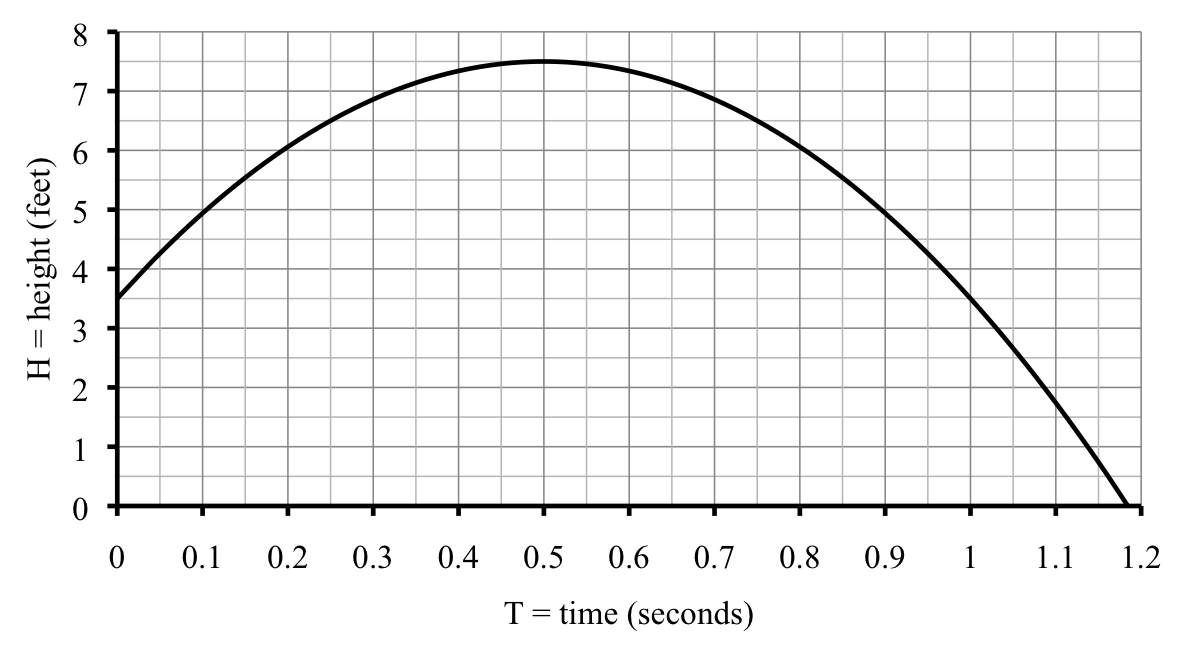
\includegraphics [width = 6in] {highjumper.png}}
\end{center}

\begin{enumerate}
\item When would the high-jumper hit the ground (if there were no pit)?  Ouch!   Use the \textsc{Quadratic Formula} to find the answer.  Use the graph to check. \vfill

\newpage %%%%%%
~\hspace{-.5in} \emph{The problem continues \ldots}

\item The high jump pit is 2 feet off the ground.  When does the high-jumper land in the pit?  Use the \textsc{Quadratic Formula} to find the answer and the graph to check. \vfill
\item How high a bar can the high-jumper clear?  Find the maximum height of that point above ground by evaluating at $\displaystyle T=\frac{-b}{2a}$.  Use the graph to check.  \vfill
\end{enumerate}

\newpage %%%%%%

\item The art museum opened in 1920.  After an initial rush to see the great holdings, attendance dropped for awhile.  But then attendance began to rise again and has risen since.  The number of annual visits $N$ is approximated by the equation $$N= 51Y^2-840Y+\text{3,700}$$ 
where $Y$ is the year since 1920.

\begin{enumerate}
\item Calculate the missing values in the table.
\begin{center}
\begin{tabular} {|c ||c |c |c |c |c |c |c |} \hline
year & 1920 & 1925 & 1930 & 1935 & 1940 & 1945 & 1950 \\ \hline
$Y$  &0 & 5& 10 & 15 & 20 & 25 & 30  \\ \hline
$N$ & \text{3,700} & \hspace{.5in}~ & 400 & \text{2,575} & \text{7,300} & \hspace{.5in}~  & \text{24,400}\\
&&&&&&&  \\ \hline
\end{tabular}
\end{center}
\item Draw a graph of the function.
\begin{center}
\scalebox {.8} {
\includegraphics [width = 6in] {GraphPaper.jpg}}
\end{center}
\bigskip
\item In what year did the number of visitors first pass \text{30,000} in a year?  Estimate the value from your graph.  Then set up and solve a quadratic equation. \vfill

\newpage %%%%%%
~\hspace{-.5in} \emph{The problem continues \ldots}

\item According to this equation, in what year was the number of annual visits the smallest?  For that year, what were the number of visits?   Use $\displaystyle T=\frac{-b}{2a}$.\vfill
\item Explain why $N$ never equals 0.  \vfill
\item What happens if you tried to use the \textsc{Quadratic Formula} to solve for $N=0$?\vfill

\end{enumerate}

\newpage %%%%%%

\item The profit \$$P$ from selling $M$ tanks of milk is described by the equation $$P=-2M^2+\text{2,000}M-\text{80,000}$$
\begin{enumerate}
\item The graph is drawn below.  Explain why negative numbers make sense. \vfill
\begin{center}
\scalebox {.9} {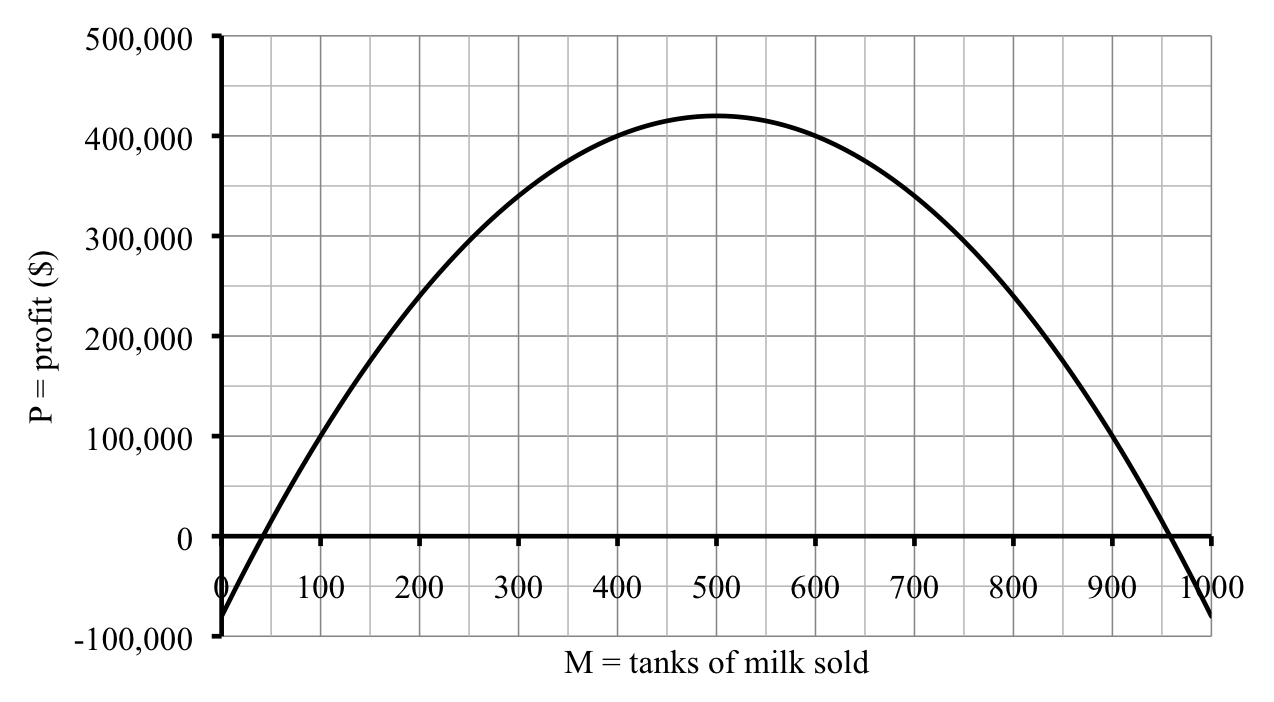
\includegraphics [width = 6in] {milk.png}}
\end{center}
\item How much milk must be sold for the company to \textbf{break even}, meaning having \$0 profit? Guess from the graph and check using the equation. \vfill
\item For practice, set up and solve a quadratic equation to find the break even point.  \vfill \vfill \vfill

\newpage %%%%%%
~\hspace{-.5in} \emph{The problem continues \ldots}

\item How many tanks of milk would they need to sell to keep profits over \$\text{400,000}?  Set up and solve a quadratic equation to find the answer.  Then check that it agrees with your graph.   \emph{Your answer should be in the form of an inequality.} \vfill
\end{enumerate}

\newpage %%%%%%

 \item Urban community gardens are catching on.  What was once an abandoned lot down the block is now a thriving 10'$\times$25' vegetable and berry garden for the neighborhood. One neighbor  volunteered to donate  gravel to make a path around the garden.  The path will be 3 inches deep and the same width all around.   
\begin{center}
\scalebox {.4} {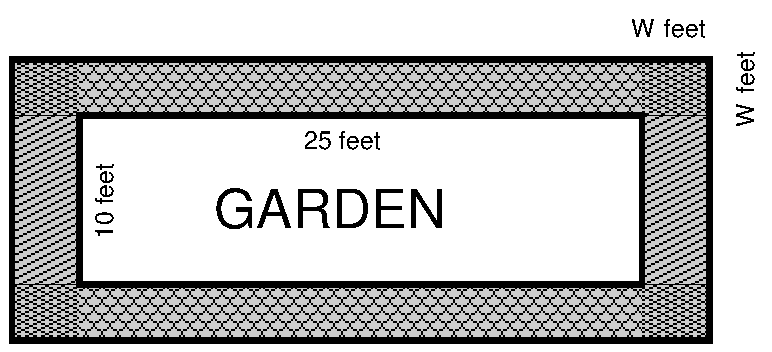
\includegraphics{GravelPath.pdf}}
\end{center}
The amount of gravel we need ($G$ cubic feet) is given by the equation  $$G = W^2 + 17.5W$$
where $W$ is the width of the path in feet.  For example, a path 4 feet wide requires 86 cubic feet of gravel, as you can check.
\hfill \emph{Story also appears in 2.3 and 2.4 Exercises}
\begin{enumerate}
\item  If the neighbor donates 60 cubic feet of gravel, how wide a path can they build?  Set up and solve a quadratic equation to find the answer to two decimal places in feet. Then convert your answer into inches. \vfill
\item Gravel is measured by the \textbf{yard}, which is short for cubic yard.  There are 27 cubic feet in 1 yard of gravel.  If the neighbor donates three yards of gravel, how wide a path can they build? Set up and solve a quadratic equation to find the answer to two decimal places in feet. Then convert your answer into inches. \vfill
\item What would it mean to solve the equation to find where $G=0$?  Can you tell what the answer is from the equation (without actually solving)? \bigskip
\end{enumerate}

\end{enumerate}

\newpage


\noindent \textbf{When you're done \ldots}

\begin{itemize}
\item [$\Box$] Check your solutions.  Still confused?  Work with a classmate, instructor, or tutor.
\item [$\Box$] Try the \textbf{Do you know} questions.  Not sure?  Read the textbook and try again.
\item [$\Box$] Make a list of key ideas and process to remember under \textbf{Don't forget!}
\item [$\Box$] Do the textbook exercises and check your answers. Not sure if you are close enough? Compare answers with a classmate or ask your instructor or tutor.  
\item [$\Box$] Getting the wrong answers or stuck?  Re-read the section and try again.   If you are still stuck, work with a classmate or go to your instructor's office hours or tutor hours.
\item [$\Box$] It is normal to find some parts of exercises difficult, but if most of them are a struggle, meet with your instructor or advisor about possible strategies or support services.
\end{itemize}





\bigskip

\noindent \textbf{Do you know \ldots} %Solving quadratic equations

\begin{enumerate} [(a)]
\item What a ``quadratic'' function is? 
\item How to solve a quadratic equation? 
\item When we use the \textsc{Quadratic Formula}?   \emph{Ask your instructor if you need to remember the \textsc{Quadratic Formula} or if it will be provided during the exam.}
\item How to solve a quadratic equation when the function is not set equal to zero? 
\item How to identify the values of $a, b, c$ in the formula? 
\item How to evaluate the formula (using your calculator)?   \item Why there are (usually) two solutions to a quadratic equation? 
\item How to decide which solution(s) from the \textsc{Quadratic Formula} are correct? 
\item What the graph of a quadratic function looks like? 
\item The value for the independent variable to find  the highest (or lowest) value of a quadratic function? 
\end{enumerate}

\bigskip

\noindent \textbf{Don't forget!}


 
%      %!TEX root =  A_WS.tex

\section*{Practice Exam 3A}  
\markright{Practice Exam 3A}  
\addcontentsline{toc}{section}{Practice Exam 3A}

Relax.  You have done problems like these before.  Even if these problems look a bit different, just do what you can.  If you're not sure of something, please ask! You may use your calculator.  Please show all of your work and write down as many steps as you can.  Don't spend too much time on any one problem.  Do well.  And remember, ask me if you're not sure about something. \bigskip

\noindent \textbf{Over 50 points on this exam are for solving equations and inequalities. Be sure you understand what you need to show for full credit.  Using a different method will get little to no partial credit.} \bigskip

\noindent \emph{As you work, make a ``don't forget'' list of any information you need to look up or ask about.} 

\noindent \hrulefill
\bigskip


\begin{enumerate} 

\item The Sk\"arstroms want to dig a new well for water for their lake cabin.  The company charges \$900 to bring the equipment on site and draw the permit and then \$2 per foot to dig.  That means $$W=900+2F$$ where $F$ is the depth of the well (in feet) and $W$ is the cost of the well (in \$).
\begin{enumerate}
\item In their neck of the woods, wells often run 200 feet deep.  According to the equation, how much would that cost? \vfill 
\item The Sk\"arstroms have budgeted between \$\text{1,500} and \$\text{1,800} for the well.  Set up and solve a chain of inequalities to find the corresponding range of depths. \vfill  \vfill \vfill 
\item No such luck.  The company had to drill much deeper than hoped to find water.  The final result, wonderfully cold and clear drinking water.  And, a hefty bill for \$\text{2,072}.  How deep is their well?  Set up and solve an equation. \vfill  \vfill \vfill% 
\end{enumerate} 

\newpage

\item Ceyda starts the day by downing two cans of Red Bull, containing a total of 160 mg of caffeine.  Her body eliminates the caffeine at a rate of 12\% each hour.  That means the amount of caffeine ($C$ mg) after $H$ hours is given by the equation graphed below  $$C= 160\ast .88^H$$ 
% Su this problem appears in 5.2 #5

\begin{center}
\scalebox {.8} {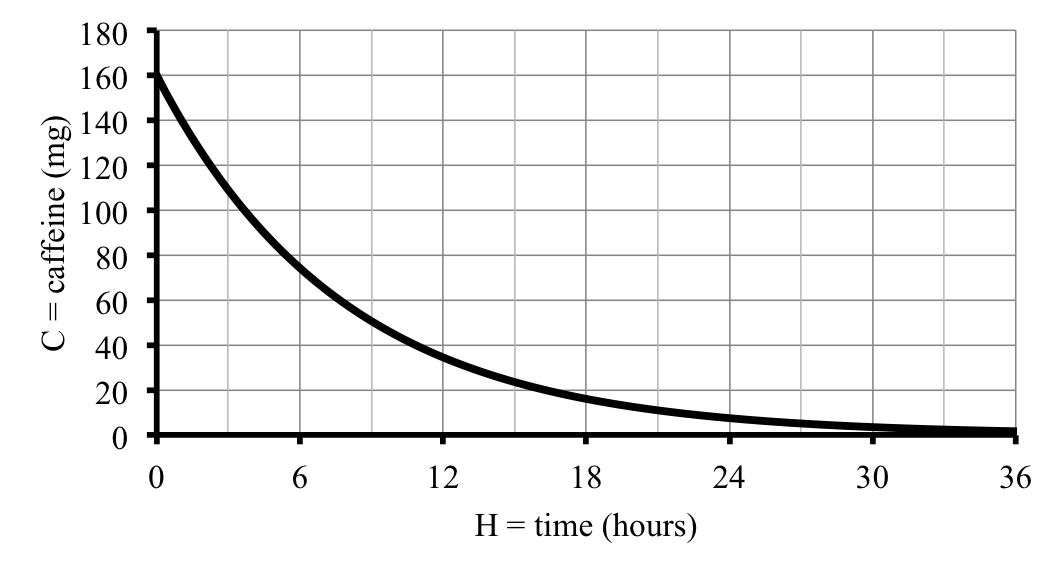
\includegraphics [width = 6in] {redbull.png}}
\end{center}

\begin{enumerate}
\item According to the equation, how much caffeine is in her body initially, after 2 hours, 5 hours, and 24 hours?  Display your answers in table.   \vfill 
\item Show show to use successive approximation to find when there will Ceyda's caffeine level first drops below 20 mg.  Answer to the nearest hour. \vfill \vfill 
\item Set up and solve an equation to determine when Ceyda's caffeine level first drops below 20 mg.  Round your answer to two decimal places. \vfill \vfill \vfill 
\end{enumerate} 

\newpage

\item Jorge deposited \$\text{1,500} in an high yield money market account and plans to leave it there for 5 years.  The value of his account after 5 years  \$$A$ will depend on the growth factor $g$ as given by the equation $$A = \text{1,500}g^5$$
\begin{enumerate}
\item Use the equation to complete the table. 

\begin{center}
\begin{tabular} {|c |c|c|c |c|}\hline
$g$ & ~ \quad 1.02 \quad ~& 1.03 & 1.05 &~ \quad 1.10\quad ~ \\ \hline
& & & & \\ 
$A$ & \text{1,656.12} & ~\hspace{1in}~&~\hspace{1in}~ & \text{2,415.77} \\  
\hline
\end{tabular}
\end{center}
\item Draw a graph showing how $A$ depends on the growth factor $g$. Start the $g$-axis at 1.00, instead of 0.
\begin{center}
\scalebox {.8} {
\includegraphics [width = 6in] {GraphPaper.jpg}}
\end{center}
\bigskip
\item Use your graph to estimate the growth factor if the value of Jorge's account after 5 years is \$\text{1,780}.  \vfill
\item Now set up and solve an equation to find the answer.  \vfill \vfill \vfill 
\item What is the corresponding \textbf{return on investment}?  That means calculate $r= g-1$.  The return on investment is $r$ written as a percentage. \vfill 
\end{enumerate} 

\newpage

\item A rabbit jumps so that her height above ground is given by the formula $$R = 17.6S - 22S^2$$ where $R=$ height of rabbit (feet above ground) and $S=$ time (seconds).
\begin{enumerate}
\item At what height did the rabbit start her jump? \vfill 
\item Can the rabbit jump over a 3 foot fence?  Calculate the exact maximum height of the rabbit to decide. \vfill \vfill 
\item How long does it take the rabbit to get 2 feet in the air and when is she at that height again? Set up and solve the appropriate equation to find the answers.  \vfill \vfill \vfill \vfill \vfill
\end{enumerate} 

%%% END

\end{enumerate}




%      %!TEX root =  A_WS.tex

\section*{Practice Exam 3B}  
\markright{Practice Exam 3B}  
\addcontentsline{toc}{section}{Practice Exam 3B}

\emph{Try taking this version of the practice exam under testing conditions:  no book, no notes, no classmate's help, no electronics (computer, cell phone, television). Give yourself one hour to work and wait until you have tried your best on all of the problems before checking any answers.} \bigskip

\noindent \textbf{Caution:} Usually more than half points on this exam are for solving equations and inequalities. Be sure you understand what you need to show for full credit.  Using a different method, or not showing enough work might get little to no partial credit. \bigskip

\noindent \hrulefill

\begin{enumerate}

\item Goldie the Goldfish, Pinches the Lobster, Quackers the Duck, Speedy the Turtle.  These first generation Beanie Babies toys were anticipated to increase in value according to the equation $$B = 6\ast1.08^Y$$ where $B$ is the value of Beanie Babies (in \$) and Y is the years since 1994. 

\hfill \begin{footnotesize} These names are registered trademarked. \end{footnotesize}
\begin{enumerate}
\item Make a table showing the anticipated value in 1994, 2004, 2010, and 2025.  \vfill 
\item Draw a graph showing how the value of the Beanie Babies increased. 
\begin{center}
\scalebox {.8} {
\includegraphics [width = 6in] {GraphPaper.jpg}}
\end{center}
\newpage
\hspace{-.5in}  \emph{The problem continues \ldots}
\item Set up and solve an equation to determine when will Beanie Babies made in 1994 were anticipated to be worth over \$40.  Report the actual year. \vfill 
\end{enumerate} 

\newpage

 \item  Best we can tell, the floor of our front porch was 7'2" above ground when the house was built.  It has been slowly sinking ever since.  The contractor estimated that it's dropped .45 inches per year.  The equation is $$P = 86-.45A$$ where $P$ is the height of the porch (in inches) and $A$ is the age of the house (in years).
\begin{enumerate}
\item Make a table showing the height of the front porch when the house was built, when it was 20 years old, and when it was 50 years old.  \vfill 
\item The floor of our front porch is currently 48 inches above ground.   Set up and solve an equation to figure out how old our house is.  \vfill \vfill 
\item Once the porch is below 40 inches, we will have to do something to fix it. Set up and solve an inequality to find when that will happen, answering to the nearest year.  \emph{Hint:  the house is already old.  Report how many years from now.} \vfill \vfill 
\end{enumerate} 

\newpage

\item In a \textbf{shot put} competition, athletes try to throw a heavy metal ball as far as possible.  For one athlete the ball closely followed the parabolic arch given by the equation $$H = -.015D^{2}+1.04D+5.9 $$ where D was the distance the ball had travelled horizontally and H was the height of the ball above ground, both in feet.  The path of the ball  is graphed below.
\begin{center}
\scalebox {.8} {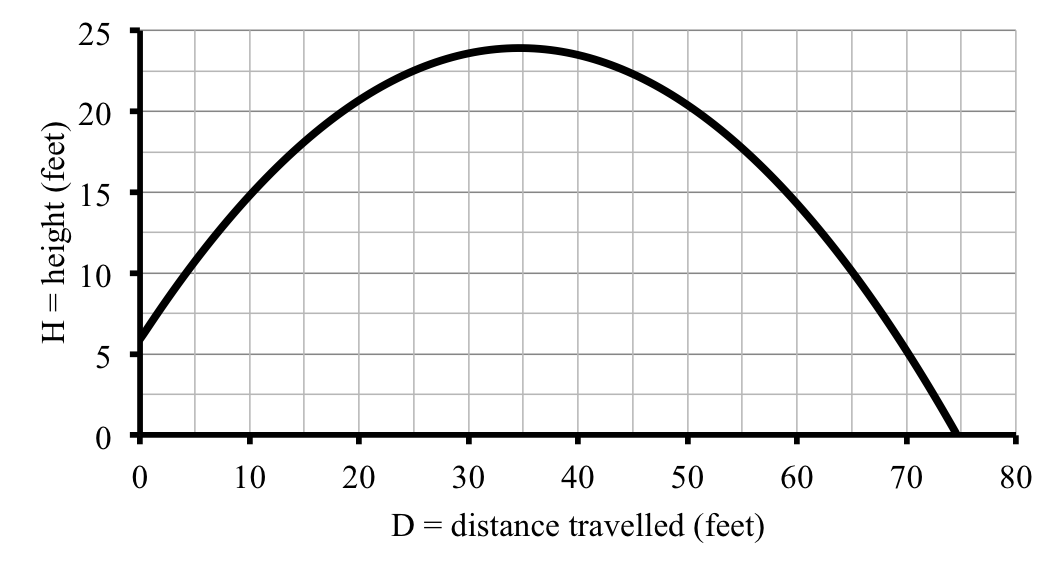
\includegraphics [width = 6in] {shotput.png}}
\end{center}

\begin{enumerate}
\item How far away did the ball land? Estimate the answer from the graph.  Then show how to set up and solve an equation to find the answer to two decimal places. \vfill \vfill \vfill  \vfill
\item How high up did the ball get?  Show how to find the exact answer.  Then compare to the graph.  \vfill 
\end{enumerate}  

\newpage

\item The amount of snow in a snowball, $C$ cups, depends on the \textbf{diameter} (distance across) of the snowball, $D$ inches according to the equation $$C = 0.036D^3$$
\begin{enumerate}
\item How many cups of snow are needed to make a snowball that is 3 inches across? 5 inches across? \vfill 
\item How many cups of snow are needed to make a snowball that is 2 feet across?
Give your answer in gallons.  Use that $1 \text{ gallon} = 4 \text{ quarts}$ and $1 \text{ quart} = 4 \text{ cups}$. \vfill
\item  Karen has a 5 gallon paint bucket packed with snow and wants to make a giant snowball out of it. How big will the snowball be? Show how to use successive approximation to find the answer to the nearest inch. Display your calculations in a table.\vfill \vfill 
\item Now set up and solve an equation to find the answer to the nearest inch. \vfill  \vfill \vfill 
\end{enumerate} 

% END
\end{enumerate}



%    
%

\chapter{A closer look at linear equations}\
    
%      %!TEX root =  A_WS.tex

\section{Modeling with linear equations  -- Practice exercises}


\begin{enumerate}
\item A solar heating system costs approximately \$30,000 to install and \$150 per year to run.  By comparison, a gas heating system costs approximately \$12,000 to install and \$700 per year to run.  \hfill \emph{Story also appears in 4.2 Exercises}

\hfill \begin{footnotesize}  Source:  ``Using Algebra'' by Ethan Bolker \end{footnotesize}
\begin{enumerate}
\item What is the total cost for installing and running a gas heating system for 30 years? \vfill  
\item Write a linear equation showing how the total cost for a gas heating system depends on the number of years you run it. \vfill  
\item Write a linear equation showing how the total cost for a solar heating system depends on the number of years you run it. \vfill  
\item If you install and run a solar heating system, how many years can you use it before it costs the same as installing and running a gas heating system for 30 years (your answer to part (a))?  Set up and solve an equation. \vfill   \vfill  
\end{enumerate}

\newpage %%%%%%

\item Since a very popular e-book reader was released, the price has been decreasing at a constant rate.  A blogger developed the following equation representing the price $E$ of the e-book reader in the months $M$ since it was released. $$E = 359 - 12M $$
\begin{enumerate}
\item Make a table of values for the e-book reader price initially, after 10 months, and after 25 months. \vfill  
\item What does the 359 mean in the story and what are its units? \vfill  
\item What does the 12 mean in the story and what are its units? \vfill  
\item Draw a graph illustrating the dependence.  
\begin{center}
\scalebox {.8} {
\includegraphics [width = 6in] {GraphPaper.jpg}}
\end{center}

\newpage %%%%%%
~\hspace{-.5in} \emph{The problem continues \ldots}

\item After approximately how many months was the price of the e-book reader expected to be down to  \$200? Set up and solve an equation. \vfill  
\item Sareth decided to purchase a e-book reader when the price fell below \$100.  How many months after its release did the price of the e-book reader fall below that level?  Set up and solve an inequality. \vfill  
\item If you can believe what you read in blogs, the manufacturer will soon be giving away the e-book reader for free, since they make money on the e-book sales themselves.  How many months after it was released would that happen, according to our equation? Set up and solve an equation. \vfill  
\end{enumerate}

\newpage %%%%%%

\item  Can you tell from the table which of these functions are linear?  Use the rate of change to help you decide.  Remember that these numbers may have been rounded.
\begin{enumerate}
\item  Savings bonds from grandpa.  \hfill \emph{Story also appears in 1.2 \#1 and 5.3 \#1} % Yes, that's a clue!

\bigskip
\begin{tabular} {|l|| c| c| c| c| c| c|} \hline
Year & 1962 & 1970 & 1980 & 1990 & 2000 & 2010\\ \hline
Value bond (\$) & 200.00 & 318.77 & 570.87 & 1,022.34 & 1,830.85 & 3,278.77 \\ \hline
\end{tabular}
\vfill


\item Wind chill at 10$^\circ$F.  \hfill \emph{Story also appears in 1.2  \#2}

\bigskip
\begin{tabular} {|l||c|c| c|c|c| c|c|c| c|c|} \hline
Wind (mph)  & 0  & 10  & 20  & 30  & 40  \\ \hline
Wind chill ($^\circ$F) & 10  & -4 & -9 & -12  & -15  \\ \hline
\end{tabular}
\vfill

\item Pizza.  \hfill \emph{Story also appears in 2.4 \#1 and 3.3 \#1}

\bigskip
\begin{tabular} {|l|| c  |c |c|}\hline
Size (inches) & 8  & 14 & 16 \\ \hline
People & 1 & 3 & 4 \\ \hline
\end{tabular} 
\vfill

\item Water in the reservoir. \hfill \emph{Story also appears in 2.1 \#2 and 3.2 Exercises}

\bigskip
\begin{tabular} {|l|| c  |c  |c |c|}\hline
Week & 1 & 5 & 10 & 20 \\ \hline
Depth (feet) & 45.5 & 39.5 & 32 & 17 \\ \hline
\end{tabular}
\vfill


\end{enumerate}

\newpage %%%%%%

\item Plumbers are really expensive, so I have been comparing prices.  James charges \$50 to show up plus \$120 per hour. Jo is just getting started in the business.  She charges \$45 to show up plus \$55 per hour.  Mario advertises ``no trip charge'' but his hourly rate is \$90 per hour. Not to be outdone, Luigi offers to unclog any drain for \$150, no matter how long it takes.  For each plumber, the table lists the corresponding equation and several points.   In each equation,  the plumber charges \$$P$ for $T$ hours of work.   \hfill \emph{Story also appears in 2.1 Exercises}
\begin{center}
\begin{tabular} {|c|| c|| c|| c|| c| } \hline
Plumber & James & Jo &~\quad Mario \quad ~& ~\quad Luigi \quad ~\\  \hline
Equation & $P=50+120T$ & $P=45+55T$ & $P=90T$ & $P=150$ \\ \hline \hline
0 hours & \$50 & \$45 & \$0 & \$150 \\ \hline
2 hours &  \$290 & \$155 & \$180 & \$150 \\ \hline
4 hours & \$530 & \$265 & \$360 & \$150  \\ \hline
\end{tabular}
\end{center}  

\begin{enumerate}
\item Use the points given to plot each of the four lines on the same set of axes.  Label each line with the plumber's name.
\begin{center}
\scalebox {.8} {
\includegraphics [width = 6in] {GraphPaper.jpg}}
\end{center}
\item What do you notice about Luigi's line? \vfill
\item List the plumbers in order from steepest to least steep line.  What does that mean in terms of the story? \vfill
\item Now list the plumbers in order from smallest to largest intercept of their line.  What does that mean in terms of the story?  \vfill
\end{enumerate}

\end{enumerate} 

\newpage


\noindent \textbf{When you're done \ldots}

\begin{itemize}
\item [$\Box$] Check your solutions.  Still confused?  Work with a classmate, instructor, or tutor.
\item [$\Box$] Try the \textbf{Do you know} questions.  Not sure?  Read the textbook and try again.
\item [$\Box$] Make a list of key ideas and process to remember under \textbf{Don't forget!}
\item [$\Box$] Do the textbook exercises and check your answers. Not sure if you are close enough? Compare answers with a classmate or ask your instructor or tutor.  
\item [$\Box$] Getting the wrong answers or stuck?  Re-read the section and try again.   If you are still stuck, work with a classmate or go to your instructor's office hours or tutor hours.
\item [$\Box$] It is normal to find some parts of exercises difficult, but if most of them are a struggle, meet with your instructor or advisor about possible strategies or support services.
\end{itemize}





\bigskip

\noindent \textbf{Do you know \ldots} % Modeling linear equations

\begin{enumerate} [(a)]
\item What makes a function linear? 
\item What the slope of a linear function means in the story and what it tells us about the graph? 
\item What the intercept of a linear function means in the story and what it tells us about the graph? 
\item The template for a linear equation?  \emph{Ask your instructor if you need to remember the template or if it will be provided during the exam.}
\item How to write a linear equation given the starting amount (intercept) and the rate of change (slope)?   
\item Where the slope and intercept appear in the template of a linear equation? 
\item What the graph of a linear function looks like? 
\item How to solve a linear equation?  
\item Why the rate of change of a linear function is constant?  
\end{enumerate}

\bigskip

\noindent \textbf{Don't forget!}


%      \section{Systems of linear equations -- Practice exercises}

\begin{enumerate}
\item Madison want to buy a new car, either the Toyota Prius, priced at \$26,100, or the Volkswagen Jetta, priced at \$23,700.  Annual fuel costs for the Toyota Prius are currently \$1,100.  For the Jetta, annual fuel costs are currently \$1,800.  The total cost of each car will depend on how many years she keeps it. 
\begin{enumerate}
\item Name the variables. \vfill
\item Write a linear equation for the total cost (including purchase price and fuel costs) of the Prius and write another linear equation for the total cost of the Jetta, each as a function of how long she keeps it.  Assume fuel costs are constant. \vfill
\item Make a table comparing the total costs for the Jetta and for the Prius if Madison keeps the car for 3, 5, or 10 years. \vfill
\item Set up and solve a system of linear equations to determine the \textbf{payoff time}, or the number of years for which the total costs of each car are equal. \vfill \vfill
\item Based on what you've learned, fill in the blank.
\begin{quote}
The more expensive Toyota Prius pays off if Madison is going to keep it for \underline{\quad~} years or more.  
\end{quote}
\end{enumerate}

\newpage %%%%%%

\item A mug of coffee costs \$3.45 at Juan's favorite cafe, unless he buys their discount card for \$10 in which case a mug costs  \$2.90.  Or, he can buy a membership for \$59.99 and then coffee is only \$1/mug.  If we let $M$ represent the number of mugs of coffee he buys and $T$ represent the total cost in dollars, then the equations are:   
\begin{center}
\begin{tabular} {ll}
\textbf{No Card:} & $T = 3.45M$ \\ 
\textbf{With Card:} & $T = 10.00 + 2.90M$ \\
\textbf{Member:} & $T=59.99+1.00M$ \\
\end{tabular}
\end{center}  
 \hfill \emph{Story also appears in 1.2 \#4 and 2.1 \#4}
\begin{enumerate}
\item Compare the total costs for all three options.
\begin{center}
\begin{tabular} {|l |c |c |c |c |} \hline
Cups &\hspace{.25in} 0\hspace{.25in} & \hspace{.25in}10\hspace{.25in} & \hspace{.25in}20\hspace{.25in} &\hspace{.25in}30\hspace{.25in} \\ \hline
&&&& \\ 
With Card &&&& \\ \hline
&&&& \\ 
No Card &&&& \\   \hline
&&&& \\ 
Member &&&& \\   \hline
\end{tabular}
\end{center}
\item Draw a graph showing all three options.
\begin{center}
\scalebox {.8} {
\includegraphics [width = 6in] {GraphPaper.jpg}}
\end{center}
\bigskip  

\item Which option is least expensive if Juan plans to buy
\begin{itemize}  \bigskip
\item A small number of mugs of coffee:  \bigskip
\item A medium number of mugs of coffee:  \bigskip
\item A large number of mugs of coffee:  \bigskip
\end{itemize}

\newpage %%%%%%
~\hspace{-.5in} \emph{The problem continues \ldots}

\item Set up and solve a system of linear equations to compare with and without the discount card. \vfill \vfill
\item Set up and solve a system of linear equation to compare the discount card to the membership. \vfill \vfill
\item Describe in words what you've learned. \vfill
\end{enumerate}

\newpage %%%%%%

\item Ahmed planted two shrubs in the backyard on May 1.  The virburnum was 16.9 inches tall and expected to grow .4 inches each week this summer.  The weigela was 20.3 inches tall but only expected to grow .2 inches per week.  If we let $S$ represent the total height of the shrub in inches after $W$ weeks, then the equations are:
\begin{center}
\begin{tabular} {ll} 
\textbf{Virburnum:} &$S=16.9+.4W$ \\
\textbf{Weigela:} & $S=20.3+.2W$ \\
\end{tabular}
\end{center}

 \hfill \emph{Story also appears in 4.1 \#4}
\begin{enumerate}
\item Compare the height of the shrub on the given dates.
\begin{center}
\begin{tabular} {|l|r|r|r|r|} \hline
date & May 1 & June 12 & July 10 & Sept 4 \\ \hline
$W$ & 0 & 6 & 10 & 18 \\ \hline
$S$ (virburnum) & &&&  \\ \hline
$S$ (weigela) & &&&\\ \hline
%$S$ (virburnum) & 16.9 & 19.3 & 20.9 & 24.1  \\ \hline
%$S$ (weigela) & 20.3 & 21.5 & 22.3 & 23.9 \\ \hline
\end{tabular}
\end{center}
\item When will the shrubs be the same height?  Continue successive approximation to find the answer to the nearest week. \vfill
\item Set up and solve an equation to find the day when the two shrubs are the same height. Report the actual calendar date. \vfill
\end{enumerate}

\newpage %%%%%%

\item The \textbf{supply} of flour is the amount of flour produced.  It depends on the price of flour.  A high price encourages producers to make more flour.  If the price is low, they tend to make less of it.  The dependence of the supply of flour S (in loads) on the price P (in \$/pound) is given by the equation %$$\textbf{supply:} \quad  S = .8 P + .5$$
\begin{center}
\begin{tabular} {ll}
\textbf{Supply:} & $S = .8 P + .5$ \\ 
\end{tabular}
\end{center}  

The \textbf{demand} of flour is the amount of flour consumers want to buy.  It also depends on the price of flour.  If flour sells for a high price, then consumers will buy less.  If flour sells for a low price instead, then consumers will buy more.  The dependence of the demand of flour D (in loads) on the price P (in \$/pound) is given by the equation %$$\textbf{Demand:} \quad D = 1.5 - .4 P$$
\begin{center}
\begin{tabular} {ll}
\textbf{Demand:} & $D = 1.5 - .4 P$ \\
\end{tabular}
\end{center}  

The \textbf{equilibrium price} of flour is the price where the supply equals the demand.  
\begin{enumerate}
\item What happens if flour is priced at \$1.00/pound?  That is, how much flour will be produced and how much will consumers want? \vfill
\item What happens if flour is priced at \$0.50/pound?  That is, how much flour will be produced and how much will consumers want? \vfill
\item Graph each dependence on the same set of axes.  What is the equilibrium price, approximately, according to your graph?

\begin{center}
\scalebox {.8} {
\includegraphics [width = 6in] {GraphPaper.jpg}}
\end{center}
\bigskip

\newpage %%%%%%
~\hspace{-.5in} \emph{The problem continues \ldots}

\item Set up and solve an equation to find the equilibrium price of flour.\vfill
\item When more of a product is produced than consumers want to buy, we have a \textbf{surplus} of the product.  Solve an inequality to find the range of price values for which there will be a surplus of flour.  Compare your answer to part (d).  \vfill
\item When less of a product is produced than consumers want to buy, we have a \textbf{shortage} of the product.  Solve an inequality to find the range of price values for which there will be a shortage of flour. Compare your answer to parts (d) and (e).  \vfill
\end{enumerate}

\end{enumerate}

%      %!TEX root =  A_WS.tex

\section{Intercepts and direct proportionality -- Practice exercises}

\begin{enumerate}

\item In each of the following stories, the temperature changes over time.  It might be confusing to call either variable $T$, so use $H$ for the time in hours and $D$ for the temperature in degrees ($^{\circ}$F).  In each case, time should be measured from the start of the story.
\begin{enumerate}
\item It was really cold at 8:30 this morning when Raina arrived at the office.  Luckily the heating system warms things up very quickly, 4$^\circ$F per hour.  By 11:00 a.m.\  it was a very comfortable 72$^\circ$ F.
\begin{enumerate}
\item Figure out what the temperature was at 8:30 a.m.  \vfill
\item Write an equation illustrating the function.   \vfill
\end{enumerate}
\item While 72$^\circ$F is a perfectly good temperature for an office, not so for ballroom dancing. When Raina arrived for her practice at 5:30 that evening, she began to sweat before she even took the floor.  Turns out the air conditioner had been running since 4:00 p.m.\ but it only cools down the room 3$^\circ$F per hour.
\begin{enumerate}
\item Figure out what the temperature was at 4:00 p.m.   \vfill
\item Write an equation illustrating the function.   \vfill
\end{enumerate} 
\end{enumerate}

\newpage %%%%%%

\item Maryn is very happy.  Her interior design business is finally showing a profit.  She has logged a total of 471 billable hours at \$35 per hour since she started her business.  Accounting for start up costs, her net profit is totals  \$\text{2,194}.

 \begin{enumerate}
\item What were Maryn's start up costs? \vfill
\item Identify the slope and intercept (including their units and sign) and explain what each means in terms of the story. \vfill
\item Calculate what Maryn's profits will be once she has logged a total of \text{1,000} hours. \vfill
\item Name the variables and write an equation relating them. \vfill
\item Graph the function.
\begin{center}
\scalebox {.8} {
\includegraphics [width = 6in] {GraphPaper.jpg}}
\end{center}
\bigskip 
\end{enumerate}

\newpage %%%%%%

\item For each story, find the initial weight of the person and use it to write an equation showing how the person's weight $P$ pounds depends on the time, $W$ weeks.
\begin{enumerate}
\item Jerome has gained weight since he took his power training to the next level ten weeks ago, at the rate of around 1 pound a week.  He now weighs 198 pounds. \vfill
\item Vanessa's doctor put her on a sensible diet and exercise plan to get her back to a healthy weight.  She will need to lose an average of 1.25 pounds a week to reach her goal weight of 148 pounds in a year.  Use $1 \text{ year} =  52 \text{ weeks}$. \vfill
\item After the past 6 weeks of terrible migrane headaches, Carlos is down to 158 pounds.  He has lost 4 pounds a week. \vfill
\item Since she has been pregnant, Zoe has gained the recommended \nicefrac{1}{2} pound per week.  Now 30 weeks pregnant and 168 pounds, she wonders if she will ever see her feet again. \vfill
\end{enumerate}

\newpage %%%%%%

\item Each story describes a situation that we are assuming is linear.  Decide whether it is \textbf{proportional}, meaning the intercept equals zero.  If it is not proportional, explain what the intercept would mean in the story. 
\begin{enumerate}
\item The price of kiwis depends on how many kiwis you buy. \emph{\textbf{Kiwi} is a fruit.} \vfill
\item The price of a bag of tortillas depends on how many tortillas are in the bag.  \vfill
\item The time it takes to vacuum a rug depends on the area of the rug.  \vfill
\item The time it takes to wash dishes depends on how many dirty dishes there are.  \vfill
\item The amount of laundry detergent I have left depends on how many loads of laundry I did. \vfill
\end{enumerate}

\end{enumerate}

\newpage


\noindent \textbf{When you're done \ldots}

\begin{itemize}
\item [$\Box$] Check your solutions.  Still confused?  Work with a classmate, instructor, or tutor.
\item [$\Box$] Try the \textbf{Do you know} questions.  Not sure?  Read the textbook and try again.
\item [$\Box$] Make a list of key ideas and process to remember under \textbf{Don't forget!}
\item [$\Box$] Do the textbook exercises and check your answers. Not sure if you are close enough? Compare answers with a classmate or ask your instructor or tutor.  
\item [$\Box$] Getting the wrong answers or stuck?  Re-read the section and try again.   If you are still stuck, work with a classmate or go to your instructor's office hours or tutor hours.
\item [$\Box$] It is normal to find some parts of exercises difficult, but if most of them are a struggle, meet with your instructor or advisor about possible strategies or support services.
\end{itemize}





\bigskip

\noindent \textbf{Do you know \ldots} % Intercepts

\begin{enumerate} [(a)]
\item What the intercept of a linear function means in the story and what it tells us about the graph? 
\item How to calculate the intercept given the slope and an example (another point on the graph)? 
\item Why an intercept might not make sense, for example if it's outside the domain of the function? 
\item When a linear function is a direct proportion? 
\item Why you cannot reason proportionally if the linear function is not a direct proportion? 
\item What the graph of a direct proportion looks like? 
\end{enumerate}

\bigskip

\noindent \textbf{Don't forget!}


%      \section{Slopes -- Practice exercises}

\begin{enumerate}
\item Jana is making belts out of leather strips and a metal clasp.  An extra short length belt (as shown) is 24.5 inches long and includes 7 leather strips.  An extra long length belt (not shown) is 37.3 inches long and includes 13 leather strips.  Each belt includes one metal clasp that is part of the total length.  All belts use the same clasp.
\begin{center}
\scalebox{.5} {
\includegraphics{leatherbelt.pdf} }
\end{center}
\begin{enumerate}
\item Name the variables, including units. \vfill
\item How long is each leather strip? \vfill
\item How long is the metal clasp?  \vfill
\item Write an equation relating the variables. \vfill
\item Solve your equation to find the number of leather strips in a extra extra long length belt that's 43.7 inches long. \vfill \vfill
\end{enumerate}

\newpage %%%%%%

\item The local ski resort is trying to set the price for season passes.  They know from past experience that they will sell around \text{14,000} passes if the season ticket price is \$380.  If the price is \$400, they will sell fewer, perhaps only \text{11,000} passes.  You can assume this decrease in demand is linear.
\begin{enumerate}
\item Name the variables.  Notice that ticket price is the independent variable. \vfill
\item How many fewer people purchase season passes for every dollar increase in the price? \vfill
\item Find the intercept.  Explain why this number does not make sense in the problem. \vfill
\item Write an equation for the function, using $T$ for the ticket price, in dollars, and $D$ for the demand (number of tickets sold). \vfill
\item How many season passes will they sell if the price is reduced to \$355? \vfill
\item The amount of \textbf{revenue} (money they take in) depends both on the ticket price and the number of tickets sold.  The equation is $R = TD$, where $R$ is the revenue, in dollars.  Calculate the revenue when ticket prices are \$355, \$380, and \$400.  \emph{That means multiply the ticket price $T$ times the number of tickets sold $D$ in each case listed.}  Of these three prices, which yields the most revenue? \vfill \vfill
\end{enumerate}

\newpage %%%%%%

\item For his Oscars party, Harland had 70 chicken wings delivered for \$51.25.  For his Super Bowl bash, Harland had 125 chicken wings delivered for \$83.70. The price includes a delivery charge. 
%slope = \$3.89/pound??? 59c/wing or 7.08/dozen
%intercept = \$17.50?
\begin{enumerate}
\item Assuming pricing is linear, what does each chicken wing cost?\vfill
\item What is the delivery charge? \vfill
\item Name the variables and write an equation for the function.\vfill
\item How many wings could Harland order for \$100?  Solve your equation.
\vfill \vfill
\item Graph and check.
\begin{center}
\scalebox {.8} {
\includegraphics [width = 6in] {GraphPaper.jpg}}
\end{center}
\bigskip 
\end{enumerate}

\newpage %%%%%%

\item Boy, am I out of shape.  Right now I can only press about 15 pounds. (\textbf{Press} means lift weight off my chest.  Literally.)  My trainer says I should be able to press 50 pounds by the end of 10 weeks of serious lifting. I plan to increase the weight I press by a fixed amount each week.
\begin{enumerate}
\item Name the variables and write an equation for my trainer's projection. 
  
 \emph{Hint:  you know the intercept.} \vfill
 \item Make a table showing my trainer's projection for after 0, 5, 10, 15, and 20 weeks.
\vfill
\item Years ago I could press 90 pounds. At this rate, when will I be able to press (at least) 90 pounds again?  Set up and solve an inequality. \vfill

\newpage %%%%%%
~\hspace{-.5in} \emph{The problem continues \ldots}

\item Draw a graph illustrating the function.
\begin{center}
\scalebox {.8} {
\includegraphics [width = 6in] {GraphPaper.jpg}}
\end{center}
\bigskip 
\bigskip 
\item I am skeptical.  I don't think I'll be able to press 50 pounds by the end of 10 weeks.  If I revise my equation, will the new slope be larger or smaller?  

 \emph{Hint:  try sketching in a possible revised line on your graph assuming that after 10 weeks I will press much less than 50 pounds.} \vfill
\item Will my revised projections mean I'll reach that 90-pound goal sooner or later?  Explain.  \emph{Hint: extend your graph.} \vfill
\end{enumerate}

\end{enumerate}


%     %!TEX root =  A_WS.tex

\section{Fitting lines to data  -- Practice exercises}

\begin{enumerate}

\item The scatter plot shows the total volume of wood, $V$ cubic feet,  in managed forests of different ages, $A$ years.  
\begin{enumerate}
\item For each line, state some reason why the fit is not good.  (We know the line will not go through all, or even most, of the points, so that is not the problem.  Instead look at slope/steepness, intercept/height, etc.) 
\end{enumerate}
 
 \begin{center}
\begin{tabular} {lcl}
LINE A & &LINE B \\ 
 \scalebox {.4} {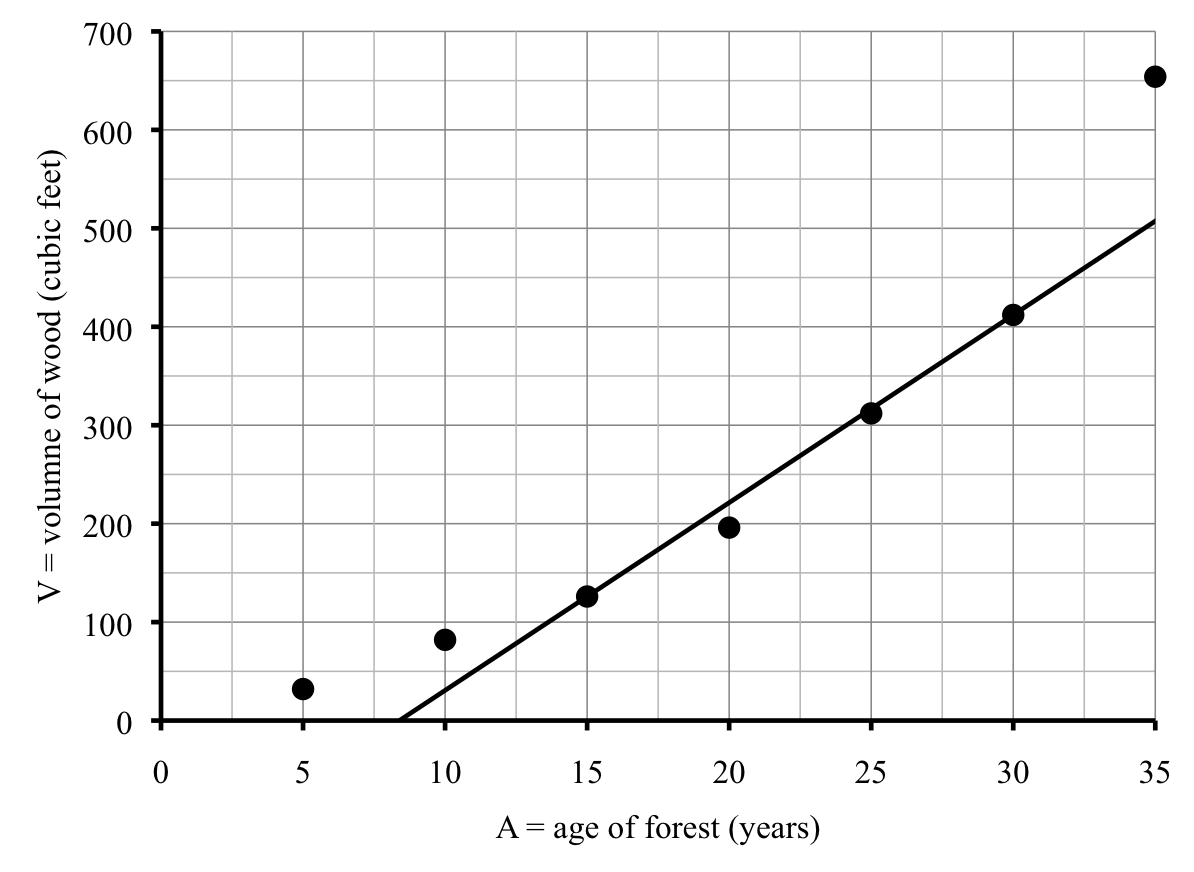
\includegraphics [width = 6in] {woodforestA.png}} 
& ~\hspace{.45in} &
 \scalebox {.4} {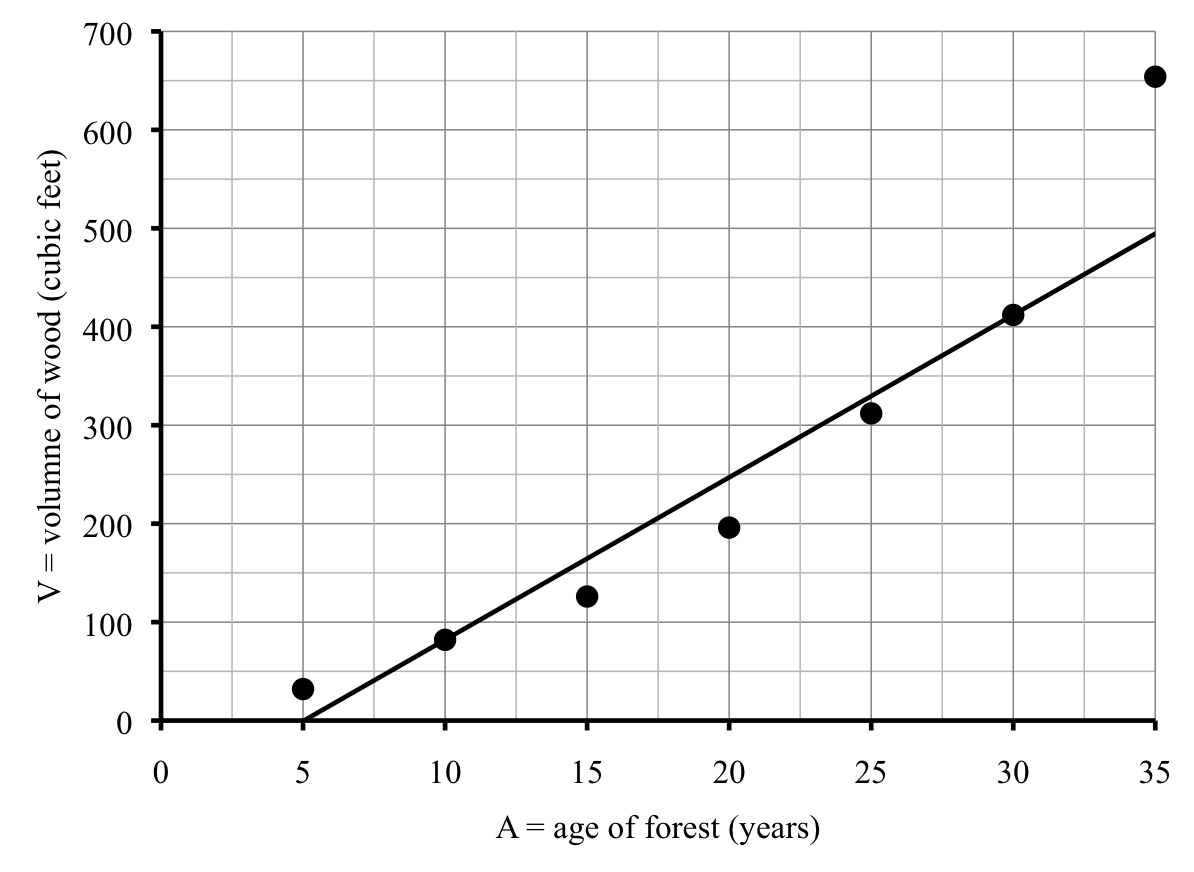
\includegraphics [width = 6in] {woodforestC.png}} \\
\end{tabular}
\end{center}
\vfill

\begin{center}
\begin{tabular} {lcl}
LINE C & & LINE D \\
 \scalebox {.4} {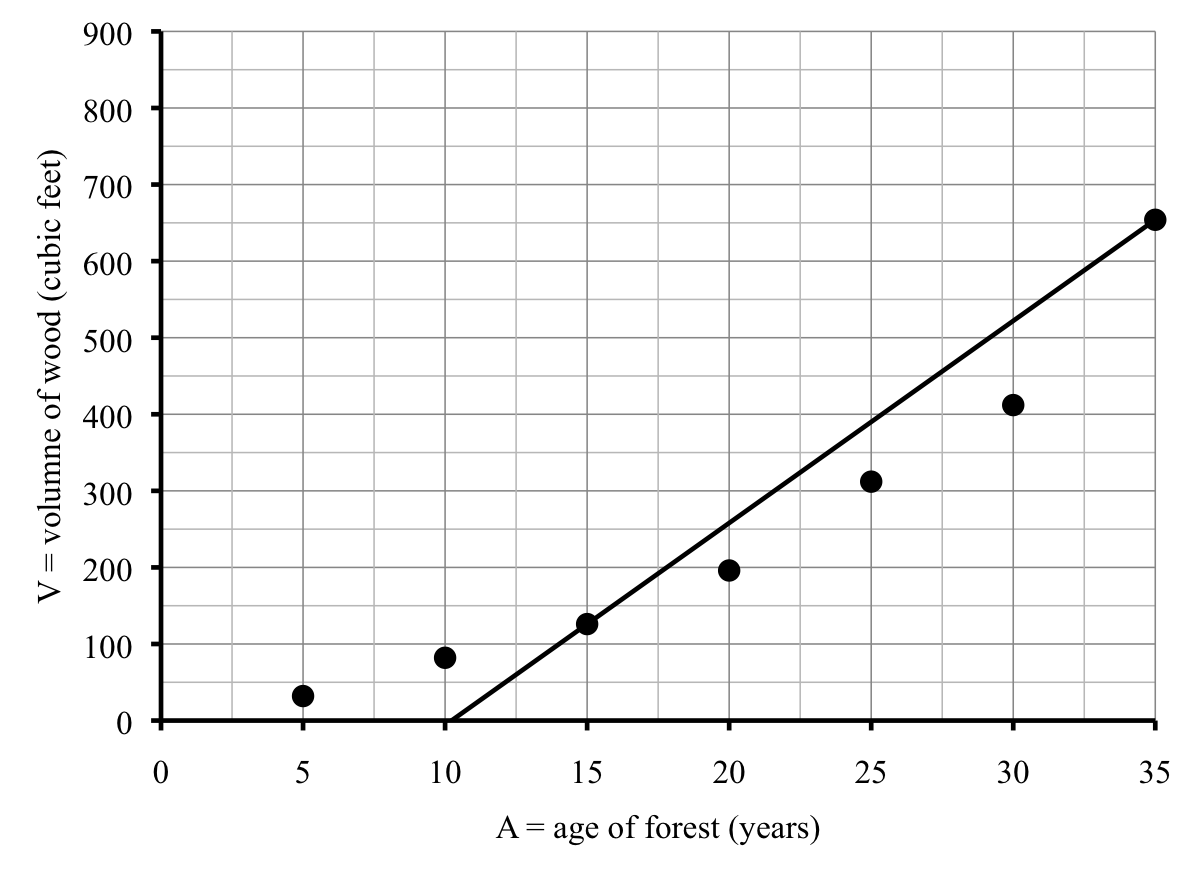
\includegraphics [width = 6in] {woodforestD.png}}
& ~\hspace{.45in} &
 \scalebox {.4} {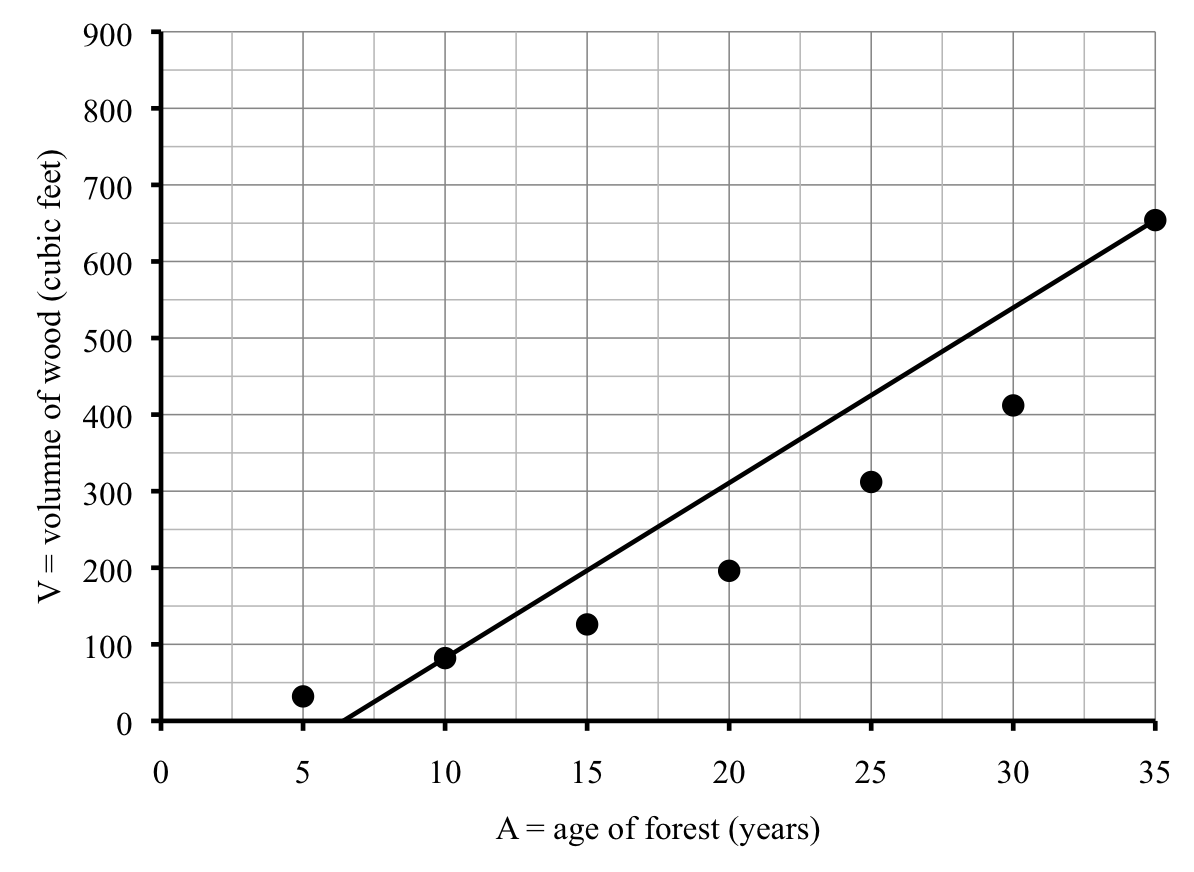
\includegraphics [width = 6in] {woodforestE.png}} \\ 
\end{tabular}
\end{center}
\vfill
\begin{enumerate}
\item [(b)] Which of these four lines do you think fits best, and why? \vfill
\end{enumerate}

\newpage %%%%%%

\item Noel is considering investing in a company's stock so he looked up a few values.
\begin{center}
\begin{tabular} {|l |c |c |c|} \hline
Day & 0 & 300 & 500 \\ \hline
Value (\$) & 23.19 & 37.00 & 48.10 \\ \hline
\end{tabular}
\end{center}
\begin{enumerate}
\item Calculate the daily rate of change of the stock's price during the first 300 days. \vfill
\item Calculate the daily rate of change of the stock's prices from Day 300 to Day 500. \vfill
\item Is this growth linear? \bigskip
\item The scatter plot shows additional values of the stock Noel is considering buying.
\begin{center}
\scalebox {.9} {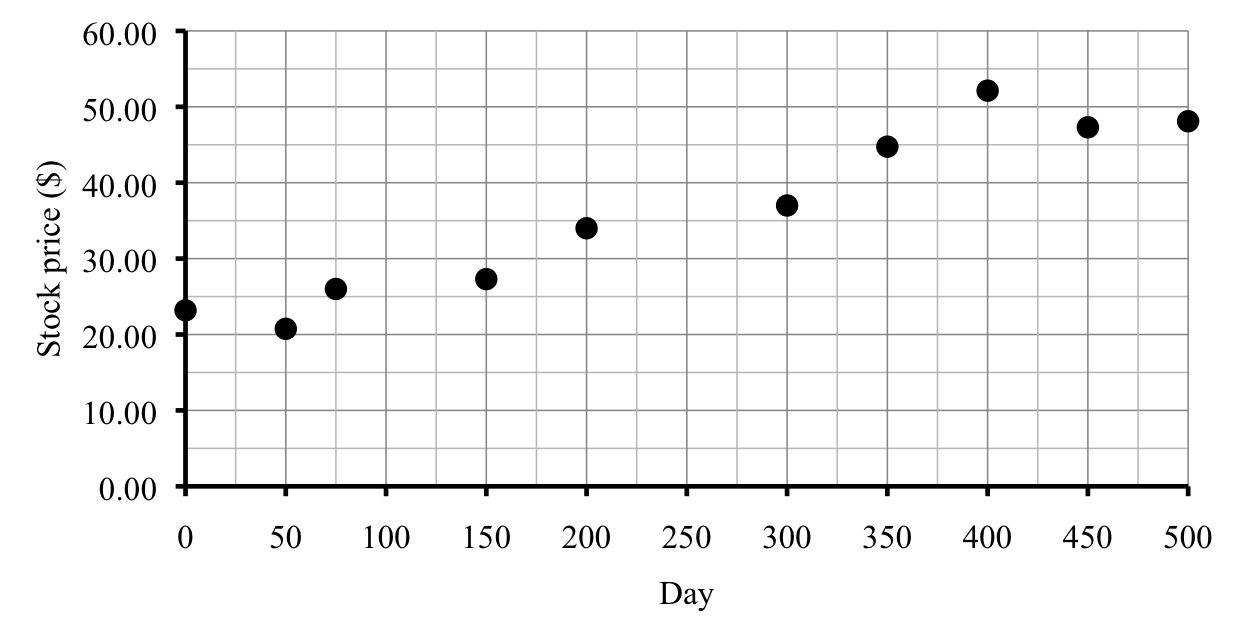
\includegraphics [width = 6in] {stockprices.png}}
\end{center}
Draw in a line that through the points for Day 300 and Day 500.  Label this line \#1.   Explain why that line does not fit the data well. \vfill
\item Draw in a line that fits the data better.  It does not need to go through any of the points exactly. Label that line \#2.  
\end{enumerate}

\newpage %%%%%%

\item Is it true that students who work part-time have lower grades?  Do the number of hours matter?  The table shows the grade point average (GPA) of ten students compared to the number of hours per week each student works at a part time job.  The variables we used are $H$, for the time worked at job (hours/week), and $G$ for the GPA, on the usual scale of 0.0 to 4.0.
\begin{center}
\begin{tabular} {|c ||c |c |c |c |c |c |c |c |c |c|}\hline
$H$ & 0&0&10&12&14&15&16&18&20&20 \\ \hline
$G$ & 3.72 & 3.91 & 3.43 & 2.79 & 3.08 & 2.62 & 2.44 & 3.17 & 3.00 & 2.55 \\ \hline
\end{tabular}
\end{center}
\begin{enumerate}
\item Make a scatter plot of the points.  Start the $G$-axis at 2.0.
\begin{center}
\scalebox {.8} {
\includegraphics [width = 6in] {GraphPaper.jpg}}
\end{center}
\bigskip

\item Find the equation of the line that goes through the first and last point listed.

\emph{Hint:  the first point tells you the intercept.}  \vfill \vfill
\item Draw this line on your graph and label it line A. 

\newpage %%%%%%
~\hspace{-.5in} \emph{The problem continues \ldots}

\item Use your equation for line A to figure out what you would expect the GPA of a student working a 30 hour per week job to be. \vfill
\item It turns out, the best fitting line has equation $G=3.7597-.0551H$.  Make a table of values for this equation using $H=0, 10, 20$ hours.  \vfill \vfill
\item Use that table of values to graph this best fitting line on that same set of axes.  Label it line B.  \bigskip
\item According to line B, what is the greatest number of hours a student should work if he or she wants to maintain a 3.5 GPA?  Solve an equation, then check on your graph. \vfill \vfill
\end{enumerate}

\newpage %%%%%%

\item Mia and Mandi and opened a candy shop this January.  The table shows their monthly sales profit.  Except for some seasonal fluctuation, Mia and Mandi generally expect your profits to rise steadily while their business is getting established.  
\begin{center}
\begin{tabular} {|c||c|c|c |c|c|c|c|c|}  \hline
Month & Jan & Feb & Mar & Apr & May & Jun & Jul  & Aug \\ \hline
Sales Profit (\$) & 3,394 & 4,702 & 3,683  & 4,840  & 5,632  & 4,432  & 4,649&  4,590 
 \\ \hline
\end{tabular}
\end{center}
\begin{enumerate}
\item Make a scatter plot.  Begin the profit axis at \$3,000.
\begin{center}
\scalebox {.8} {
\includegraphics [width = 6in] {GraphPaper.jpg}}
\end{center}
\bigskip
\item Name the variables and write an equation for the line through January and August.  Add this line (\#1) to your graph.  This line is too low. \vfill \vfill

\newpage %%%%%%
~\hspace{-.5in} \emph{The problem continues \ldots}

\item Write an equation for the line through March and July.  Notice that you need to find the intercept this time.  Add this line (\#2) to your graph.  This line is too steep. \vfill \vfill \vfill
\item Neither of these lines go anywhere near the data for February, April, and May, because those are outliers.  Any idea why those months had much higher candy sales than the other months? \vfill
\item What does each equation give as an estimate for September's sales?  \vfill
\item Explain why Mia and Mandi should not use either of these lines to estimate October's sales. \vfill
\end{enumerate}

\end{enumerate}

\newpage


\noindent \textbf{When you're done \ldots}

\begin{itemize}
\item [$\Box$] Check your solutions.  Still confused?  Work with a classmate, instructor, or tutor.
\item [$\Box$] Try the \textbf{Do you know} questions.  Not sure?  Read the textbook and try again.
\item [$\Box$] Make a list of key ideas and process to remember under \textbf{Don't forget!}
\item [$\Box$] Do the textbook exercises and check your answers. Not sure if you are close enough? Compare answers with a classmate or ask your instructor or tutor.  
\item [$\Box$] Getting the wrong answers or stuck?  Re-read the section and try again.   If you are still stuck, work with a classmate or go to your instructor's office hours or tutor hours.
\item [$\Box$] It is normal to find some parts of exercises difficult, but if most of them are a struggle, meet with your instructor or advisor about possible strategies or support services.
\end{itemize}





\bigskip

\noindent \textbf{Do you know \ldots} %Fitting_lines_to_data

\begin{enumerate} [(a)]
\item What a scatter plot is? 
\item Why we might begin the scale for a scatter plot somewhere other than 0?
\item Why we would approximate data with a linear function? 
\item How to decide visually whether a line is a reasonable approximation of the data? 
\item The name for a point that falls very far away from an approximating line? 
\item How to graph a line from its equation by creating a table first.
\item Why even the best fitting line doesn't go through most of the data points?
\end{enumerate}

\bigskip

\noindent \textbf{Don't forget!}



%Wood forest earlier versions:
%
%LINE A \\
% \scalebox {.4} {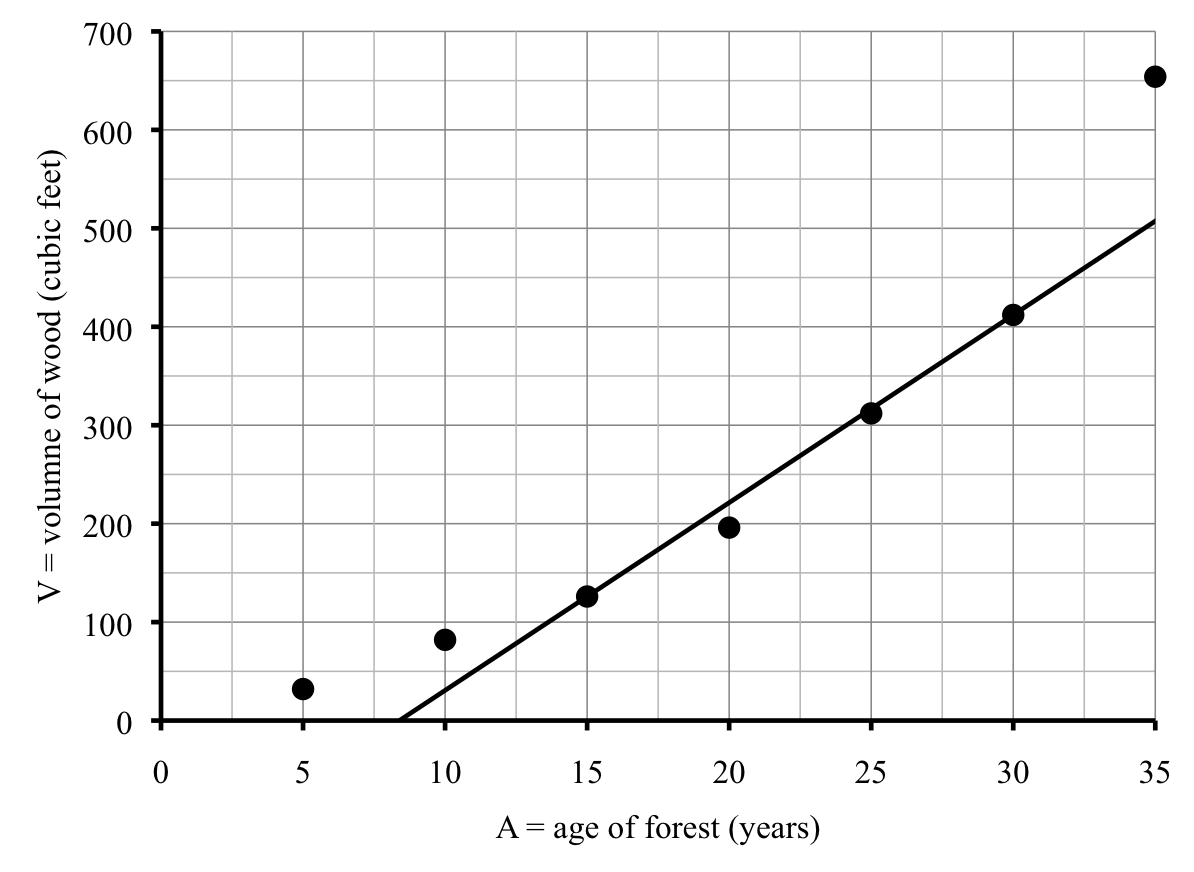
\includegraphics [width = 6in] {woodforestA.png}} 
% 
%LINE B \\
% \scalebox {.4} {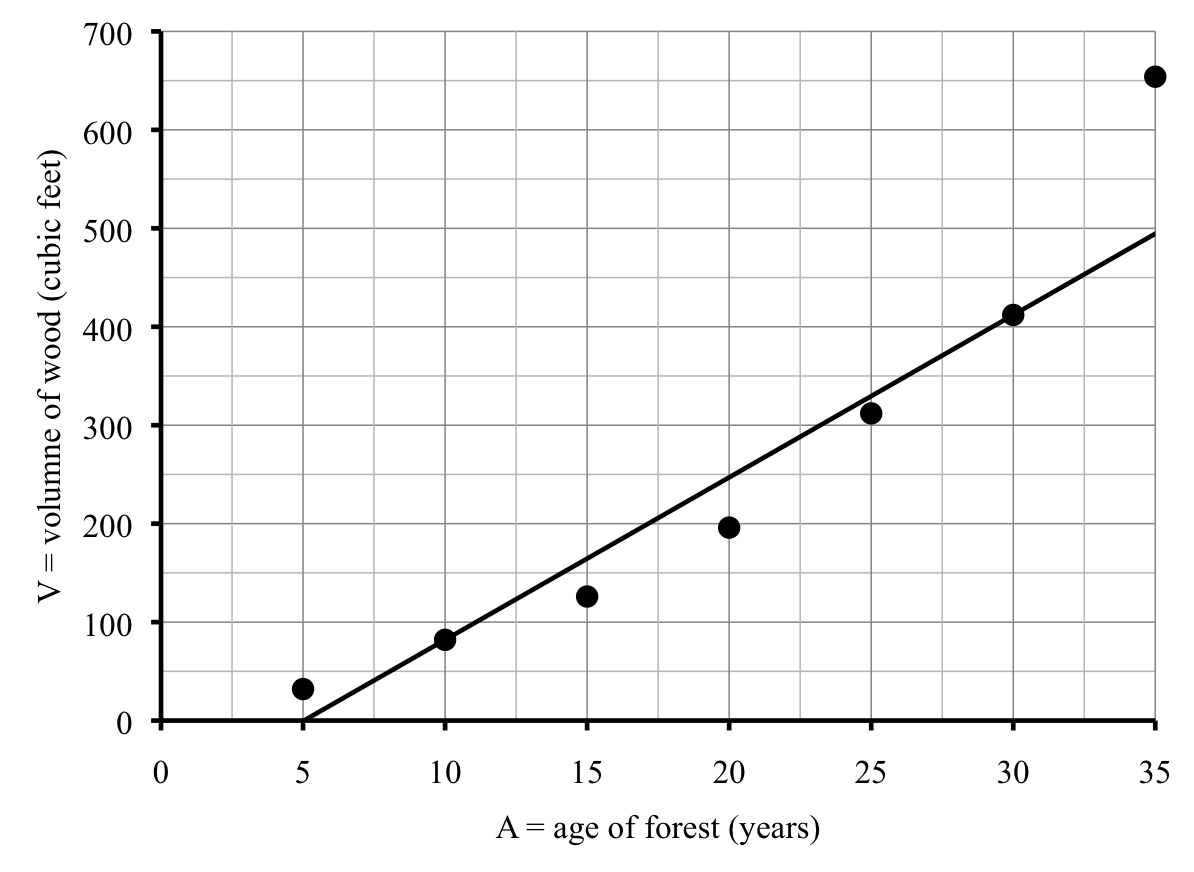
\includegraphics [width = 6in] {woodforestC.png}}

%LINE C \\
% \scalebox {.4} {\includegraphics [width = 6in] {woodforestD.png}}
% 
%LINE D \\
% \scalebox {.4} {\includegraphics [width = 6in] {woodforestE.png}}
%%%%%%

%\item The following table shows the total volume of wood, $V$ cubic feet,  in managed forests of different ages, $A$ years.
%\begin{center} 
%\begin{tabular} { |c| |c |c |c |c |c |c |c|} \hline
%$A$ & 5 & 10 & 15 & 20 & 25 & 30 & 35 \\ \hline
%$V$ & 32 & 82 & 126 & 196 & 312 & 412 & 654 \\ \hline
%\end{tabular}
%\end{center}
%For each line drawn, decide if it's a good fit or not.  If not, explain why.
%\bigskip

%      %!TEX root =  A_WS.tex

\section*{Practice Exam 4A}  
\markright{Practice Exam 4A}  
\addcontentsline{toc}{section}{Practice Exam 4A}

Relax.  You have done problems like these before.  Even if these problems look a bit different, just do what you can.  If you're not sure of something, please ask! You may use your calculator.  Please show all of your work and write down as many steps as you can.  Don't spend too much time on any one problem.  Do well.  And remember, ask me if you're not sure about something. \bigskip

\noindent \emph{As you work, make a ``don't forget'' list of any information you need to look up or ask about.} 

\noindent \hrulefill
\bigskip


\begin{enumerate} 

\item Forde collects miniature cars, each weighing 1.76 ounces.  His car box weighs 4 ounces when empty.  The total weight $T$ ounces of Forde's car box depends on the number of cars $C$ according to the equation $$T=4+1.76C$$
%Forrest's candy bucket weighs 4 ounces when empty.  Each Snickers Almond\footnote{For those who can remember, Snickers Almond is essentially the old Mars Bar renamed.  But, I digress.} bar he puts in his bucket weighs 1.76 ounces.   The total weight $T$ ounces of Forrest's candy bucket depends on the number of Snickers Almond bars $B$ according to the equation $$T=4+1.76B$$
\begin{enumerate}
\item Make a table of values showing the weight if it contains 1, 5, 12, or 20 cars.
\vfill
\item Draw a graph illustrating the dependence.  
\bigskip
\begin{center}
\scalebox {.8} {\includegraphics [width = 6in] {GraphPaper.jpg}}
\end{center}
\bigskip
\item How many cars can Forde fit in the box and stay under 3 pounds (that is 48 ounces)? 
Figure out the answer and mark the corresponding point on your graph.
\vfill 
\end{enumerate} 

\newpage

\item  Will women ever run the marathon as fast as men do?  The world records are getting close.  In 2012 the men's record was 2:03:38 and the women's record was 2:15:25, about 12 minutes apart!  On the other hand, the record is changing very slowly.  Estimates for the men's time shows about 13 seconds drop per year on average.  Estimates for the women's time shows about 26 seconds drop per year on average.

\hfill \begin{footnotesize} Source:  Wikipedia (Marathon World Record Progression) \end{footnotesize}
%Data from wikipedia shows Men's record 2003 = 2:04:55, then 2007 = 2:04:26, then 2008=2:03:59, and then 2011=2:03:38.  For the women it's 199 = 2:20:43, then 2001 = 2:19:46, then 2002 = 2:17:18, and then 2003 = 2:15:25.
\begin{enumerate}
\item Write an equation for each function:  men's and women's.  Use $T$ for the marathon times (in seconds) and $Y$ for the years (measured in years since 2012).  Note that 2:03:38 $= 7,418 $ seconds and 2:12:25 $= 7,945$ seconds. 
\vfill
\item Use successive approximate to estimate when the women's record might equal the men's record.  Display your guesses in a table.
\vfill
\item Set up and solve a system to estimate when the women's record might equal the men's record. 
\vfill 
\end{enumerate} 

\newpage

\item An online music club charges a monthly enrollment fee plus \$.95 per album you download.  Last month Andrew downloaded 31 albums for a total cost of \$49.00.  
\begin{enumerate}
\item What is the monthly enrollment fee?  
\vfill
\item Name the variables, including units, and write an equation relating them. 
\vfill
\item If the bill next month is for \$87.95, how many albums did Andrew download? Show how to solve the equation
\vfill
\end{enumerate} 

\newpage

\item A report  shows September sea-ice declining in the Northern hemisphere. In 1980 the extent of the sea-ice was 3.1 million square miles.  By 2012, the sea-ice extended only 1.7 million square miles.  For this problem, suppose that the area of sea-ice decreases linearly. 
\hfill \begin{footnotesize} Source: National Snow and Ice Data Center \end{footnotesize}
\begin{enumerate}
\item Name the variables, including units. 
\vfill
\item What is the rate of sea ice decrease? 
\vfill
\item Write a linear equation relating your variables. 
\vfill
\item Scientists are concerned that if the September sea-ice falls between 200,000 and 500,000 square miles, then other climate feedbacks will lead to no more sea-ice in September.  According to your equation, in what year is this expected to occur?  Set up and solve an inequality to answer the question. 
\vfill
\end{enumerate} 

\newpage

\item  As people age they experience some hearing loss.  A study was done to determine the \textbf{comfort level of sound} for people of different ages, meaning the loudest sound (in decibels) that the person could listen to comfortably.  The data are given in the table.
\begin{center}
\begin{tabular} {|l ||c |c |c |c |c |c |c |c |} \hline
Name & Akbar & Javier & Walter & Xang & Rolf & Derrick & Iago &Raheem \\ \hline
Age & 45 & 45 & 55 & 65 & 75 & 75 & 85 & 85\\ \hline
Comfort level & 58 & 61 & 63 & 71 & 75 & 80 & 82 & 79 \\ \hline
\end{tabular}
\end{center}
\begin{enumerate}
\item Make a scatterplot showing the data.  Scale your axes to start at 40 years and start the level at 55 decibels.  Spread out your scale to get a large, detailed graph.
\bigskip
\begin{center}
\scalebox {.8} {\includegraphics [width = 6in] {GraphPaper.jpg}}
\end{center} 
\bigskip
\item  Draw the line through the points listed for Xang and Rolf.  Explain why that line does not fit the data well.  \emph{Label this line B.} 
\vfill
\item  The ``best-fitting line'' from statistics has equation $$C=34.315+.5556A$$ where $A$ is the person's age (in years) and $C$ is the comfort level (in decibels).  Make a table showing the values of $C$ when $A = 40, 60,$ and $80$.  Use those points to add this ``best-fitting line'' to your graph. 
\vfill
\vfill
\end{enumerate} 

%%% END

\end{enumerate}


%      %!TEX root =  A_WS.tex

\section*{Practice Exam 4B}  
\markright{Practice Exam 4B}  
\addcontentsline{toc}{section}{Practice Exam 4B}

\emph{Try taking this version of the practice exam under testing conditions:  no book, no notes, no classmate's help, no electronics (computer, cell phone, television). Give yourself one hour to work and wait until you have tried your best on all of the problems before checking any answers.}

\noindent \hrulefill

\begin{enumerate}

\item The Vang family wants to buy a new washing machine.  The first model costs \$645 and then \$13.29 per month to run.  A more efficient model costs \$940 and then \$7.82 per month to run.  If $M$ is the number of months and $V$  is the Vang family's total cost  (in \$), then the equations and some comparable values (to the nearest \$) are:
\vspace{-.25in} 
\begin{center}
\begin{tabular} {ll} \\
\textbf{First model:} &$V = 645 + 13.29M$ \\ 
\textbf{Second model:}  & $V = 940 + 7.82M$ \\ 
\end{tabular}
\end{center}

\begin{center}
\begin{tabular} {|l||r|r|r|} \hline
$M$ & 12 & 36 & 60 \\ \hline
\textbf{First model:} & 804.48  & \text{1,123.44} &  \text{1,442.40}  \\ \hline
\textbf{Second model:} &  \text{1,033.84} &  \text{1,221.52} &  \text{1,409.20} \\ \hline
\end{tabular}
\end{center}

\begin{enumerate}
\item Draw a graph illustrating both equations. \emph{Be sure to include the intercepts.}
\bigskip
\begin{center}
\scalebox {.8} {\includegraphics [width = 6in] {GraphPaper.jpg}}
\end{center} 
\bigskip
\item According to your graph, approximate what is the  \textbf{payback time} (the number of months for which the total costs of each washing machine are equal)?   Answer and indicate the point on the graph where you can check. 
 
\newpage %%
 
\hspace{-.5in}  \emph{The problem continues \ldots}
 
\item Set up and solve a system of linear equations to find the payback time.  
\vfill
\item If the manufacturer offers a \$25 rebate on the more efficient model, how does that change the payback time? Adjust your equation and set up and solve a new system.  Or carefully explain some other way of figuring it out.  
\vfill 
\vfill
\end{enumerate} 
\newpage

\item It has been a long time since anyone broke the record for the men's long jump.  In 1935 Jesse Owens jumped  8.13 meters.  The record was next broken 25 years later, in 1960, by Ralph Boston who jumped 8.21 meters. He broke his own record several times over the next few years, including being surpassed briefly by Igor Ter-Ovanesyan.  Ralph's final record was 8.35 meters in 1965. Not to be outdone, Igor tied the record in 1967. Then in 1968, Bob Beamon jumped 8.90 meters.  That record held for 23 years, until Mike Powell jumped 8.95 meters in 1991, much to Carl Lewis' dismay.  Powell's record still stood 21 years later, in 2012. \hfill \begin{footnotesize} Source:  Wikipedia (Long Jump) \end{footnotesize}
% source:  http://en.wikipedia.org/wiki/Long_jump
\begin{center}
\scalebox {.8} {\includegraphics [width = 6in] {longjump.png}}
\end{center} 
\begin{enumerate}

\item Draw in the line connecting the data from 1935 and 1991.  Use it to predict the long jump record in 2020. 
\vfill
\item Draw in the line connecting the data from 1968 and 1991.  Use it to predict the long jump record in 2020. 
\vfill
\item Which of your lines do you prefer, and why?  
\vfill
\end{enumerate} 

\newpage

\item Arjun just graduated from college but is living with his uncle for the summer to save money.  They agreed that Arjun would do chores and some light renovations instead of paying rent.  Arjun has been doing around 5 hours of work a week for the past 8 weeks, but still owes his uncle another 30 hours of work.
\begin{enumerate}
\item What was the original agreement? That means, how many hours of work did Arjun promise his uncle? 
\vfill
\item Name the variables and write an equation relating them, assuming Arjun continues to do 5 hours a week of work. 
\vfill

\item How many more weeks will it take Arjun to finish the work he promised?  Show how to solve the equation. 
\vfill
\vfill
\end{enumerate} 

\newpage

\item The local zoning commission is considering a plan to expand housing in the city, as measured in the number of residential units.  But with more residential units come more shops, offices, schools, recreational facilities, churches, and other commercial property. Currently the city has \text{3,500} residential units and \text{1,575} acres of commercial property.  If the proposal is passed and completed, the city will have a new total of \text{3,600} residential units and \text{1,620} acres of commercial property.  You can assume this increase is linear.
\begin{enumerate}
\item Name the variables and summarize the given information in a table. 
\vfill
\item How many new acres of commercial property are there for each new residential unit built? 
\vfill
\item Write an equation relating the variables. \emph{Hint:  first find the intercept.}
\vfill
\vfill
\item If the city decides to limit the amount of land to \text{1,600} acres of commercial property, approximately how many residential units can there be?  Use successive approximation, displaying your guesses in a table.
\vfill
\item Now answer the question by setting up and solving an inequality. 
\vfill
\end{enumerate} 

% END

\end{enumerate}

%      
%

\chapter{A closer look at exponential equations}


%      %%!TEX root =  A_WS.tex

\section*{Formulas for Chapter 5}  
\markright{Formulas for Chapter 5}  
\addcontentsline{toc}{section}{Formulas for Chapter 5}

 \bigskip
 \bigskip
\noindent \hrulefill
 \bigskip
 \bigskip
 
\noindent  \textsc{Log-Divides Formula:} \quad
The equation $g^Y = v$ has solution $\displaystyle Y = \frac{\log (v)}{\log(g)}$

 \bigskip
 \bigskip
\noindent \hrulefill
 \bigskip
 \bigskip
 
\noindent \textsc{Percent Change Formula:} 
\begin{itemize}
\item   If a quantity changes by a percentage corresponding to growth rate $r$, then the growth factor is $$\displaystyle g=1+r$$
\item If the growth factor is $g$, then the growth rate is $$r = g-1$$ ~
\end{itemize}

~\vspace{-.5in} %VSPACE

\noindent \hrulefill
 \bigskip
 \bigskip
 
\noindent \textsc{Growth Factor Formula:}
If a quantity is growing (decaying) exponentially, then the growth (decay) factor is 
$$\displaystyle g = \sqrt[t]{\frac{a}{s}}$$ where $s$ is the starting amount and $a$ is the amount after $t$ time periods. 

 \bigskip
 \bigskip
\noindent \hrulefill
 \bigskip
 \bigskip
 
\vfill




%      \section{Modeling with exponential equations -- Practice exercises}

\begin{enumerate}
\item The population of Buenos Aires, Argentina in 1950 was estimated at 5.0 million and expected to grow at 1.8\% each year.  \hfill \begin{footnotesize} Source: Mongabay \end{footnotesize}
\begin{enumerate}
\item Name the variables. \vfill
\item What is the annual growth factor? \vfill
\item Write an equation estimating the population of Buenos Aires over time. \vfill
\item Make a table of values showing the estimated population of Buenos Aires every 20$^{\text{th}}$ year from 1950 to 2030. \vfill \vfill \vfill
\item By how many people has the population been increasing during each 20 year period? Add these numbers to your table. As expected, these numbers change because the rate of change is not constant.
\item The actual population of Buenos Aires in the year 2000 was around 12.6 million and by 2010 it was around 15.2 million.  How does that compare to the estimates? \vfill
%(This now includes a larger surrounding area as the city has spread beyond historical limits.)  
%\item Would it surprise you to know that recent growth rates are closer to 10\%?  
\end{enumerate} 

\newpage %%%%%%

\item A flu virus has been spreading through the college dormitories. Initially 8 students were diagnosed with the flu, but that number has been growing 16\% per day.   Earlier we found the equation $$N=8 \ast1.16^D$$ where $D$ is the number of days (since the first diagnosis) and $N$ is the total number of students who had the flu.   \hfill  \emph{Story also appears in 2.2 \#3 and 5.5}

\begin{enumerate}
\item Use successive approximations to estimate when the number of infected students reaches 100. Display your guesses in a table. \vfill
\item Use the \textsc{Log Divides Formula} to solve your equation.  \vfill
\item There are 1,094 students currently living in the dorms.  Suppose ultimately 250 students catch the flu.  According to your equation, when would that happen?  Show how to solve your equation. \vfill
\item It is not realistic to expect that everyone living in the dorms will catch the flu, but what does the equation say?  Set up and solve an equation to find when all 1,094 students would have the flu.  (Again, this is not realistic.) \vfill
\end{enumerate}

\newpage %%%%%%

\item Bunnies, bunnies, everywhere.   Earlier we found the equation $$B = 1,800\ast 1.13^Y$$ where $B$ is the number of bunnies and $Y$ is the years since 2007. 

\hfill  \emph{Story also appears in 2.2 \#2}
\begin{enumerate}
\item Make a table showing the number of bunnies in 2007, 2010, 2013, and 2020.  \vfill 
\item Draw a graph showing how the bunny population grew.
\begin{center}
\scalebox {.8} {\includegraphics [width = 6in] {GraphPaper.jpg}}
\end{center}
\bigskip
\item When will the population pass 5,000 bunnies?  Guess from the graph. Then refine your answer using successive approximation.  \vfill
\item Show how to solve your equation to get the answer.  \vfill 
\end{enumerate}  

\newpage %%%%%%

\item Carbon dioxide is a greenhouse gas in our atmosphere.  Increasing carbon dioxide concentrations are related to global climate change. In 1980, the carbon dioxide concentration was 338 ppm (parts per million).   At that time it was assumed that carbon dioxide concentrations would increase .42\% per year. 
%That means about one million molecules of air contained 338 molecules of carbon dioxide).

 \hfill \begin{footnotesize} Source: Earth Systems Research Laboratory, NOAA \end{footnotesize}
%ftp://ftp.cmdl.noaa.gov/ccg/co2/trends/co2_annmean_mlo.txt
\begin{enumerate}
\item Name the variables including units.     \vfill
\item Assuming the growth is exponential as predicted, write an equation that describes the increase in carbon dioxide concentrations.   \vfill
\item The carbon dioxide concentration in 2008 was 385 ppm. Is that count higher or lower than predicted from your equation?  Explain.   \vfill
\item Does that mean that carbon dioxide increased at a higher or lower rate than .42\%?  Explain.   \vfill
\end{enumerate}

\end{enumerate}
 
%      \section{Exponential growth and decay -- Practice exercises}

\begin{enumerate}

\item A signal is sent down a fiber optic cable. It decreases in strength by 2\% each mile it travels.  (Say it was one unit strong to start.)
\begin{enumerate}
\item Make a table showing the strength of the signal over the first five miles. \vfill
\item Name the variables, including units, and write an equation relating them.  \vfill
\item The signal will need a \textbf{booster} (something to make the signal stronger again) when it has fallen to under .75 units. How far along the cable should the booster be placed?  Set up and solve an equation.  \vfill

\newpage %%%%%%
~\hspace{-.5in} \emph{The problem continues \ldots}

\item What's the half-life (or should we say half-distance) of a signal?  That means, how far can it travel without dropping below 50\%?  (That won't actual happen because we'd boost the signal.)  Again, set up and solve an equation.  \vfill
\item Draw a graph illustrating the relationship.
\begin{center}
\scalebox {.8} {\includegraphics [width = 6in] {GraphPaper.jpg}}
\end{center}
\bigskip
\item  Indicate the points on your graph where you can check your answers to parts (c) and (d). 
\end{enumerate}

\newpage %%%%%%

\item A recent news report stated that cell phone usage is growing exponentially in developing countries.  In one small country, \text{50,000} people owned a cell phone in the year 2000.  It was estimated that usage would increase at 1.4\% percent per year.

\begin{enumerate}
\item Name the variables including units.  \vfill
\item Assuming the growth is exponential, write an equation for the function.  \vfill
\item At this rate, how many years would it take for the number of people owning a cell phone to double?  That's called the  \textbf{doubling time}.  Show how to set up and solve an equation to find the answer.  \vfill   \vfill
\item In 2011, about \text{682,000} people owned a cellphone.  Is that count higher or lower than predicted from your equation?  Explain.  \vfill
\item Based on the 2011 data, would you say that cell phone usage was growing slower or faster than 1.4\%?  \vfill
\end{enumerate}

\newpage %%%%%%

\item  If a person has a heart attack and his or her heart stops beating, the amount of time it takes paramedics to restart his or her heart with a defibrillator is critical.  Each minute that passes decreases the person's chance of survival by 10\%.  Assume that this statement means the decrease is exponential and that the survival rate is 100\% if the defibrillator is used immediately. \hfill \begin{footnotesize} Source: American Red Cross \end{footnotesize}
\begin{enumerate}
\item Name the variables and write an equation. \vfill
\item If it takes the paramedics 2 minutes to use the defibrillator, what is the person's chance of survival? \vfill
\item When does the survival rate drop below 50\%? Use successive approximation to estimate to the nearest minute.  Display your work in a table. \vfill \vfill
\item Solve your equation. \vfill \vfill
\end{enumerate}  
%http://www.redcross.org/prepare/location/workplace/easy-as-aed

\newpage %%%%%%

\item You and two buddies each invite 10 people to ``like'' your online group.  Suppose everyone accepts and then they each invite 10 people.  And then everyone accepts and they each invite 10 people.  And so on. Of course, there is likely to be substantial overlap, but for the moment pretend that there isn't.  
\begin{enumerate}
\item There are 3 friends to start.  In the first round they each invite 10 friends, so a total of 30 new people ``like'' your online group in the first round.  How many new people ``like'' your group in the second round?  The third? \vfill
\item Name the variables and write an equation showing how the number of new people increases in each round. Think of the original 3 friends as round 0.\vfill \vfill
\item Make a table showing this information. Continue your table to include the number of new people who ``like'' your group in the fourth and fifth rounds. \vfill 
\item What is the \emph{total} number of people who ``like'' your online group after five rounds.  \emph{Hint: add} \vfill
\item Comment on why our assumption is unrealistic. \vfill
\end{enumerate} 

\end{enumerate}

%      %!TEX root =  A_WS.tex

\section{Growth factors -- Practice exercises}

\noindent \hrulefill
 \bigskip
 
 \noindent \textsc{Percent Change Formula:} 
\begin{itemize}
\item   If a quantity changes by a percentage corresponding to growth rate $r$, then the growth factor is $$\displaystyle g=1+r$$
\item If the growth factor is $g$, then the growth rate is $$r = g-1$$ ~
\end{itemize}
 
\noindent \textsc{Growth Factor Formula:} \bigskip

If a quantity is growing (decaying) exponentially, then the growth (decay) factor is 
$$\displaystyle g = \sqrt[t]{\frac{a}{s}}$$ 
\quad where $s$ is the starting amount and $a$ is the amount after $t$ time periods.

\bigskip 
 \noindent \hrulefill
 
\newpage %%%%%%
 
\begin{enumerate}

\item In 1962, my grandfather had savings bonds that matured  to \$200.  He gave those to my mother to keep for me.  These bonds have continued to earn interest at a fixed, guaranteed rate so I have yet to cash them in.  The table lists the value at various times since then.  
\begin{center}
\begin{tabular} {|c|| c| c| c| c| c| c|} \hline
year & 1962 & 1970 & 1980 & 1990 & 2000 & 2010\\ \hline
$Y$ & 0 & 8 & 18 & 28 & 38 & 48\\ \hline
$B$ & 200.00 & 318.77 & 570.87 & 1,022.34 & 1,830.85 & 3,278.77 \\ \hline
\end{tabular}
\end{center}   \hfill  \emph{Story also appears in 1.2 \#1 and 4.1 \#3}

\begin{enumerate}
\item Use the \textsc{Growth Factor Formula} to find the annual growth factor for the time period from 1962 to 1970.  \vfill
\item Repeat for 1970 to 1980.    \vfill
\item What do you notice?  What in the story told you that would happen?  \vfill
\item What is the corresponding interest rate?   \vfill
\item Write an equation for the value of bonds over time.  \vfill
\item Use your equation to check the information for 1990, 2000, and 2010.  \vfill

\newpage %%%%%%
~\hspace{-.5in} \emph{The problem continues \ldots}

\item In what year will the bond be worth over \$5,000?  Set up and solve an equation to decide.  \vfill  \vfill
\item Draw a graph using the data in the table, but not your answer to part (g).  Include another year that is later than your answer to part (g).  
\begin{center}
\scalebox {.8} {\includegraphics [width = 6in] {GraphPaper.jpg}}
\end{center}
\bigskip
\item Does your answer to part (g) agree with your graph?  If not, fix your work. 
\end{enumerate}  

\newpage %%%%%%

\item Have you read news stories about archaeological digs where a specimen (like a bone) is found that dates back thousands of years?  How do scientists know how old something is?  One method uses the radioactive decay of carbon.  After an animal dies the carbon-14 in its body very slowly decays.  By comparing how much carbon-14 remains in the bone to how much carbon-14 should have been in the bone when the animal was alive, scientist can estimate how long the animal has been dead.  Clever, huh?  Actually, it is so clever that Willard Libby won the Nobel Prize in Chemistry for it.  The key information to know is that the half-life of carbon-14 is about 5,730 years. For this problem, suppose a bone were found that should have contained 300 milligrams of carbon-14 when the animal was alive. 
\hfill \begin{footnotesize} Source:  Wikipedia (Radiocarbon Dating)  \end{footnotesize}
\begin{enumerate}
\item Find the annual ``growth'' factor. Keep as many digits as possible for your calculations.  \vfill
\item Name the variables and write an equation describing the dependence. \vfill
\item How many milligrams of carbon-14 should remain in this bone after 1,000 years? After 10,000 years? After 100,000 years?  \vfill
\item How many milligrams of carbon-14 should remain in this bone after 1 million years?  Explain the answer your calculator gives you.  \vfill

\newpage %%%%%%
~\hspace{-.5in} \emph{The problem continues \ldots}

\item Draw a graph that shows up to 10,000 years. 
\begin{center}
\scalebox {.8} {\includegraphics [width = 6in] {GraphPaper.jpg}}
\end{center}
\bigskip

\item If the bone is determined to have 100 milligrams of carbon-14, how old is it? That is, approximately how long ago did it die? Start by estimating the answer from your graph.  Then revise your estimate using successive approximation.  Display your guesses in a table. \vfill
\item Solve the equation exactly. \vfill \vfill
\end{enumerate}

\newpage %%%%%%

\item For each story, find the annual growth factor $g$ and annual growth rate $r$ as a percent.  

\emph{Hint:  First decide if you can use the \textsc{Percent Change Formula} or if you will need to use the \textsc{Growth Factor Formula}.}

\emph{Don't forget to include the negative sign for decay rates.}
\begin{enumerate}
\item  Donations to the food shelf have increased 35\% per year for the past few years. 
\vfill
~\hfill $g=$ \hspace{1in} 

~\hfill $r=$ \hspace{1in} 
\vfill
\item  People picking up food at the food shelf has increased exponentially too, from 120 per week in 2005 to 630 per week in 2011. \vfill
~\hfill $g=$ \hspace{1in} 

~\hfill $r=$ \hspace{1in} 
\vfill

\item The crime rate has dropped 3\% each year recently. \vfill
~\hfill $g=$ \hspace{1in} 

~\hfill $r=$ \hspace{1in} 
\vfill

\item The new stop sign has decreased accidents exponentially, from 40 in 2008 to 17 in 2013. \vfill
~\hfill $g=$ \hspace{1in} 

~\hfill $r=$ \hspace{1in} 
\vfill
\newpage %%%%%%
~\hspace{-.5in} \emph{The problem continues \ldots}

\item The creeping vine taking over Fiona's lawn will double in area each year. \vfill
~\hfill $g=$ \hspace{1in} 

~\hfill $r=$ \hspace{1in} 
\vfill
\item Attendance at parent volunteer night has doubled every 3 years.\vfill
~\hfill $g=$ \hspace{1in} 

~\hfill $r=$ \hspace{1in} 
\vfill

\item The number of people addicted to prescription drugs was estimated to have tripled in the past 5 years.  Assume the number is increasing exponentially.  \vfill
~\hfill $g=$ \hspace{1in} 

~\hfill $r=$ \hspace{1in} 
\vfill

\item The number of high school students arrested for driving under the influence is half what it was 5 years ago.  Assume the number is falling exponentially.  \vfill
~\hfill $g=$ \hspace{1in} 

~\hfill $r=$ \hspace{1in} 
\vfill

\end{enumerate}

\newpage %%%%%%

\item For each equation, find the growth rate and state its units. For example, something might ``grow 2\% per year'' while something else might ``drop 7\% per hour''  %Use the \textsc{Percent Change Formula}.

\begin{enumerate} 

\item The number of households watching reality television $R$ (in millions) was estimated by the equation $$R=2.5 \ast 1.072^Y$$ where $Y$ is the years since 1990. 
\hfill \emph{Story also appears in 5.1 Exercises} \vfill

\item Chlorine is often used to disinfect water in swimming pools, but  the concentration of chlorine $C$ (in ppm) drops as the swimming pool is used for $H$ hours according to the equation $$C = 2.5 \ast .975^H$$ 
 \hfill  \emph{Story also appears in 3.4 \#2} \vfill
 
 \item The number of players of a wildly popular mobile app drawing game  has been growing exponentially according to the equation $$N = 2 \ast 1.57^W$$ where $N$ is the number of players (in millions) and $W$ is the number of weeks since people started playing the game.
 \hfill \emph{Story also appears in 5.1 Exercises} \vfill
 % Source: Wikipedia (Draw Something) 5 weeks 20 million, 50 days 50 million
 
\end{enumerate}

\end{enumerate}

\newpage


\noindent \textbf{When you're done \ldots}

\begin{itemize}
\item [$\Box$] Check your solutions.  Still confused?  Work with a classmate, instructor, or tutor.
\item [$\Box$] Try the \textbf{Do you know} questions.  Not sure?  Read the textbook and try again.
\item [$\Box$] Make a list of key ideas and process to remember under \textbf{Don't forget!}
\item [$\Box$] Do the textbook exercises and check your answers. Not sure if you are close enough? Compare answers with a classmate or ask your instructor or tutor.  
\item [$\Box$] Getting the wrong answers or stuck?  Re-read the section and try again.   If you are still stuck, work with a classmate or go to your instructor's office hours or tutor hours.
\item [$\Box$] It is normal to find some parts of exercises difficult, but if most of them are a struggle, meet with your instructor or advisor about possible strategies or support services.
\end{itemize}





\bigskip

\noindent \textbf{Do you know \ldots} %Growth_factor

\begin{enumerate} [(a)]
\item How to find the growth/decay factor given the starting amount and another point of information? 
\item How to find the growth/decay factor given the doubling time or half-life? 
\item When we use the \textsc{Percent Change Formula}, and when we use the \textsc{Growth Factor Formula} instead?  \emph{Ask your instructor if you need to remember the \textsc{Percent Change Formula} and \textsc{Growth Factor Formula} or if they will be provided during the exam.}
\item How to evaluate the \textsc{Percent Change Formula} and \textsc{Growth Factor Formula} using your calcuator? 
\item How to read the starting amount and percent increase/decrease from the equation? 
\end{enumerate}

\bigskip

\noindent \textbf{Don't forget!}


%      \section{Linear vs.\ exponential models -- Practice exercises}

\begin{enumerate}

\item My parents bought the house I grew up in for \$35,000 and sold it 40 years later for \$342,000. True story.  (It was before the housing bubble burst.)

\textbf{First, assume the value of the house increased exponentially.}
\begin{enumerate}
\item Calculate the annual growth factor. \vfill
\item In this model, by what percentage did the house value increase each year?  \bigskip
\item Write an exponential equation showing how the value of the house increased.   Don't forget to name the variables, including units. \vfill 
\item Check that your equation gives the correct sold value. \bigskip
\end{enumerate}

\textbf{Next, assume the value of the house increased linearly instead.}
\begin{enumerate} 
\item [(e)] In this model, by what fixed amount did the house value increase each year?  \emph{Hint:  calculate the slope.} \vfill
\item [(f)] Write a linear equation showing how the value of the house increased.  \vfill
\item [(g)] Check that your equation gives the correct sold value.  \bigskip
\end{enumerate}

\newpage %%%%%%

\item The number of manufacturing jobs in the state has been declining for decades. In 1970, there were 1.2 million such jobs in the state but by 2010 there were only .6 million such jobs.   Write $J$ for the number of manufacturing jobs (in millions) and $Y$ for the years since 1970.

\textbf{First, assume the number of jobs decreased linearly.}
\begin{enumerate}
\item Calculate the slope. \vfill
\item Write a linear equation showing how the number of jobs declined.  \vfill
\item Check that your equation gives the correct value for 2010. \bigskip
\end{enumerate}

\textbf{Next, assume the number of jobs decreased exponentially instead.}
\begin{enumerate} 
\item [(d)] Calculate the growth factor. \vfill
\item [(e)] Write an exponential equation showing how the number of jobs declined. \vfill
\item [(f)] Check that your equation gives the correct value for 2010. \bigskip
\end{enumerate}

\newpage %%%%%%
~\hspace{-.5in} \emph{The problem continues \ldots}

\textbf{Now, compare the models.}
\begin{enumerate} 
\item [(g)] Complete the table of values. 
\begin{center}
\begin{tabular} {|c| |c |c |c |c |c|}\hline
year &  ~\hspace{.05in}1970\hspace{.05in} ~ & ~\hspace{.05in} 1990 \hspace{.05in} ~&  ~\hspace{.05in} 2010 \hspace{.05in} ~& ~\hspace{.05in} 2020 \hspace{.05in} ~& ~\hspace{.05in} 2030 \hspace{.05in} ~\\ \hline
$Y$ &  0 & 20 & 40 & 50 & 60\\ \hline
$J$ (if linear) &  & &  & & \\ 
&&&&& \\ \hline
$J$ (if exponential) &  & &  & & \\ 
&&&&& \\ \hline
\end{tabular}
\end{center}
\bigskip
\item [(h)] Draw a graph showing both models.  
\begin{center}
\scalebox {.8} {\includegraphics [width = 6in] {GraphPaper.jpg}}
\end{center}
\bigskip
\item [(i)] Which model has better news for 2030? \bigskip
\end{enumerate}

\newpage %%%%%%

\item In December 2010, a popular mobile app game featuring animated birds launched from slingshots  had 50 million downloads.  Six months later (May 2011), the game had 200 million downloads.  
Let $D$ denote the number of downloads of the game (in millions) and $M$ the months since December 2010.  
\begin{enumerate}
\item Suppose that the number of downloads have been increasing at a \emph{constant rate each month}.   What type of equation is suggested here?  Write that equation and use it to estimate the number of downloads in November 2011 (when $M=11$). \vfill
\item Suppose that the number of downloads have been increasing at a \emph{fixed percentage each month}. What type of equation is suggested here?  Write that equation and use it to estimate the number of downloads in November 2011 (when $M=11$). \vfill\end{enumerate}

\newpage %%%%%%

\item Bus fares are up to \$2.25 per ride during rush hour. Two different plans of increasing fares are being debated: 10\textcent~per year or 2.5\% per year. 
 \begin{enumerate}
\item Make a table comparing these plans over the next \textbf{decade} (ten years). \vfill
\item Draw a graph showing both options.
\begin{center}
\scalebox {.8} {\includegraphics [width = 6in] {GraphPaper.jpg}}
\end{center}
\bigskip
\item As a city council representative, you want to support the plan that your constituents prefer.  If most of your constituents ride the bus, which plan should you support? \vfill
\item If most of your constituents are members of the same union as the bus drivers (who count on solid earnings from the bus company to keep their jobs), then which plan should you support? \vfill

\newpage %%%%%%
~\hspace{-.5in} \emph{The problem continues \ldots}

\item Which type of equation is being suggested in each plan? Write the equations.  Don't forget to name the variables, including units. \vfill \vfill \vfill \vfill
\end{enumerate}
\end{enumerate}

%      \section{Logistic and other growth models -- Practice exercises}  

\begin{enumerate}

\item Corn farmers say that their crop is healthy if it is ``knee high by the Fourth of July.''  An equation that relates the height $H$ (in inches) of the corn crop $D$ is days since May 1 is $$H=106-100 \ast .989^{D} $$ %Saturating

\begin{enumerate}
\item According to this equation, how high is corn expected to be on the Fourth of July (day 64)?  Is that ``knee high''? Let's say that's 18 inches tall.  \vfill
\item These days with stronger corn from cross-breeding and various seed technologies, the rule ought to be modified to ``chest high.''  Let's say that's 52 inches tall.  According to this equation, on approximately what date is the corn projected to be that tall?  Use successive approximation to answer. \vfill
\item The particular corn matures in approximately 110 days (by August 19).  How tall will it be then?  \vfill
\item Draw a graph of the function.  Include when $D=0$.
\begin{center}
\scalebox {.8} {\includegraphics [width = 6in] {GraphPaper.jpg}}
\end{center}
\end{enumerate}

\newpage %%%%%%

\item An alternative equation for corn height is  $$H = \frac{200}{1+70\ast.965^D}$$ %Logistic
\begin{enumerate}
\item According to this new equation, how high is corn expected to be on the Fourth of July (day 64)?  Is that ``knee high'' (18 inches tall)?  \vfill
\item According to this new equation, on approximately what date is the corn projected to be ``chest high''  (52 inches tall)?  Use successive approximation to answer.  \vfill
\item The particular corn matures in approximately 110 days (by August 19).  How tall will it be then?   \vfill
\item Add the graph of this function to your graph of the original equation.
\end{enumerate}

\newpage %%%%%%

 \item Following the 2011 Japanese earthquake and tsunami there was concern of radiation leaking from nuclear power plants.  Suppose that a monitoring station recorded radiation approximated by the equation
$$R=\frac{.162}{1+3319\ast.3127^T}$$ % Logistic
 where $R$ is radiation measured in milliSieverts (mSv) and $T$ is time in hours.
 \begin{enumerate}
\item How much radiation was detected at the start? After 24 hours?  48 hours? \vfill
\item Approximately when did the radiation level off? (Display your work in a table.) What was the largest amount of radiation at that time? \vfill
\item The normal level of radiation that a person is exposed to around 2.4 mSv during an entire  year.  What is that normal level of radiation measured in mSv/day?  Use $1 \text{ year} = 365 \text{ days}$. \hfill \begin{footnotesize} Source:  Wikipedia (Sievert) \end{footnotesize}  \vfill
\item At its largest amount (where it leveled off), did the radiation the exceed normal daily levels?  If so, by how many times normal?  

\emph{That means divide your answer to (b) by your answer to (c).} \vfill
\end{enumerate}
% Ask John if it's 1.62 or really .162.  They will be a little freaked out Helpful facts: Chest x-ray .05 milliSieverts, 2.4 milliSieverts = average amount of  natural radiation
%near the Fukushima Daiichi 

\newpage %%%%%%

\item Jason works at a costume shop selling Halloween costumes.  The shop is busiest during the fall before Halloween.  An equation that describes the number of daily visitors $V$ the shop receives $D$ days from August 31 is the following:
$$ V=\frac{430}{1+701\ast .81^D}$$ % Logistic
An alternative equation is $$V = 700 - 690 \ast .985^D$$ %Saturating
\begin{enumerate}
\item Make a table showing what each equation predicts for August 31, September 15, September 30, October 15, October 25, October 28, and October 31. 

\emph{Hint:  those days are numbered 0, 15, 30, 45, 55, 58, and 61.} \vfill
\item Graph both functions on the same set of axes.
\begin{center}
\scalebox {.8} {\includegraphics [width = 6in] {GraphPaper.jpg}}
\end{center}
\bigskip
\item Which function is more consistent with a major advertising campaign that aired starting the first week of September?  Explain. \vfill
\end{enumerate}


\end{enumerate}

\newpage

~

%      %!TEX root =  A_WS.tex

\section*{Practice Exam 5A}  
\markright{Practice Exam 5A}  
\addcontentsline{toc}{section}{Practice Exam 5A}

Relax.  You have done problems like these before.  Even if these problems look a bit different, just do what you can.  If you're not sure of something, please ask! You may use your calculator.  Please show all of your work and write down as many steps as you can.  Don't spend too much time on any one problem.  Do well.  And remember, ask me if you're not sure about something. \bigskip

\noindent \emph{As you work, make a ``don't forget'' list of any information you need to look up or ask about.} 

\noindent \hrulefill
\bigskip

\begin{enumerate} 

\item Leopard print hat. Originally 5 out of \text{1,000} women shopping at a major retail store even looked twice.  But that number grew and grew, by my estimate around 40\% a week, thanks to carefully placed ads in fashion magazines.
\begin{enumerate}
\item Write an equation illustrating the interest in leopard print hats using $W$ for the time (in weeks) and $L$ for the number of women interested in leopard print hats (women per thousand). 
\vfill
\item Make a table showing the number of women, per thousand female shoppers, who stop and look at the hat at the start, 1 week, 2 weeks, and 3 weeks after it hits the stores. 
\vfill
\item The leopard print hat is considered popular when more than 300 out of \text{1,000} women try it on.  According to the equation, when will the hat be considered popular?  Use successive approximation to find the answer to the nearest week and display your guesses in a table. 
\vfill
\vfill
\item The hat will be considered pass\'e when over 750 out of \text{1,000} women try it on.  I mean -- everyone's got one!  According to your equation, when will that happen?  Set up and solve an equation, again answering to the nearest week. 
\vfill
\vfill
\end{enumerate} 

\newpage

\item HeeChan bought a classic car in 2003 for investment purposes and has been watching the value increase over the years.  Based on the data, HeeChan came up with two possible equations
$$\textbf{Logistic:} \quad C= \frac{\text{41,000}}{1+4\ast.81^Y}$$

$$ \textbf{Saturation:} \quad C = \text{32,000}-\text{23,800}\ast.85^Y$$

where $Y$ is the years since 2003 and \$$C$ is the value of the car.

\begin{enumerate}
\item How much did HeeChan pay for the car in 2003? 
\vfill
\item What does each equation predict for the value of the car in 2013?  In 2020?   
\vfill
\item What does each equation say will be the eventual value long term?  \emph{Hint:   if you are not sure try 100 years.}  
\vfill
\end{enumerate} 

\newpage

\item The number of geese in the Twin Cities metropolitan area increased from 480 in 1968 to \text{25,000} in 1994.  Although population is sometimes modeled with exponential models, there are many factors that might make an exponential model inappropriate, such as changes in migration, wetlands, and hunting.
\begin{enumerate}
\item Name the variables. 
\vfill
\item Write a linear equation modeling the goose population. 
\vfill
\vfill
\item Now write an exponential equation modeling the goose population. 
\vfill
\vfill

\newpage
\hspace{-.5in} \emph{The problem continues \ldots}

\item Compare the models projections for 1968, 1975, 1984, 1994, 2000, 2010, and 2020.  Summarize your findings in a table. 
\vfill
\vfill
\item Graph each function over the period from 1968 to 2020 on the same set of axes.   

\emph{Test-taking tip:  even if you have trouble with the equations, you should be able to plot the information given in the story and sketch in the appropriate shape curves.}

\bigskip
\begin{center}
\scalebox {.8} {\includegraphics [width = 6in] {GraphPaper.jpg}}
\end{center} 
\bigskip

\item Research indicates that the Twin Cities metropolitan area could support \text{60,000} geese.  Use your graph to estimate when that will happen. 
\vfill
\item The actual goose population in 2010 was around \text{50,000}.  Which model was closer? 
\vfill
\end{enumerate}  

\newpage

 \item  One of the toxic radioactive elements produced by nuclear power plants is strontium-90. A large amount of strontium-90 was released in the nuclear accident at Chernobyl in the 1980's.  The clouds carried the strontium-90 great distances. The rain washed it down into the grass, which was eaten by cows. People then drank the milk from the cows.  Unfortunately, strontium-90 causes cancer. Strontium-90 is particularly dangerous because it has a half-life of approximately 28 years, which means that every 28 years half of the existing strontium-90 changes into a safe product; the other half remains strontium-90. Suppose that a person drank milk containing 100 milligrams of strontium-90.

\hfill \begin{footnotesize}Source:  ``Explorations in College Algebra,'' by Kime and Clark\end{footnotesize}
\begin{enumerate}
\item After 28 years, how many milligrams of strontium-90 remains in the person's body? After 56 years? 
\vfill
\item Find the annual percentage decrease of strontium-90. 
\vfill
\vfill
\item Name the variables and write an equation relating them. 
\vfill
\vfill
\item Suppose that any amount under 20 milligrams of strontium-90 is considered ``acceptable'' in humans. Will it have reached acceptable levels after 70 years? 
\vfill
\end{enumerate}  

%%% END

\end{enumerate}





%      %!TEX root =  A_WS.tex

\section*{Practice Exam 5B}  
\markright{Practice Exam 5B}  
\addcontentsline{toc}{section}{Practice Exam 5B}

\emph{Try taking this version of the practice exam under testing conditions:  no book, no notes, no classmate's help, no electronics (computer, cell phone, television). Give yourself one hour to work and wait until you have tried your best on all of the problems before checking any answers.}

\noindent \hrulefill

\begin{enumerate}

\item The number of school children in the district whose first language in not English has been on the rise.  The equation describing the situation is $$C=673(1.043)^Y$$ where $C$ is the number of school children in the district whose first language is not English, and $Y$ is the number of years (from now).
\begin{enumerate}
\item Make a table showing the number of school children in the district whose first language is not English now, in one year, in two years, and in ten years. \emph{Don't forget now too.} 
\vfill
\vfill
\item What percent increase is implicit in this equation?
\vfill
\item Use successive approximation to determine when there will be over \text{1,700} school children in the district whose first language is not English Display your work in a table.  Round your answer to the nearest year. 
\vfill
\vfill
\item Show how to solve the equation to calculate when there will be over \text{1,700} school children in the district whose first language is not English. 
\vfill
\vfill
\end{enumerate}  

\newpage

\item The lottery jackpot started at \$600,000.  After 17 days the jackpot had increased to \$2.1 million.  The lottery is designed so that the jackpot grows exponentially.

\begin{enumerate}
\item Name the variables including units. 
\vfill
\item Write an equation describing the jackpot.  \emph{Hint:  find the daily growth factor.} 
\vfill
\vfill
\item By what percentage does the jackpot increase each day? 
\vfill
\item What will the jackpot be after 20 more days (after 37 days total)? 
\vfill
\end{enumerate} 

\newpage

\item The creeping vine is taking over Fiona's front lawn.  Write $V$ for the area covered by the vine (in square feet) and $Y$ for the years since she moved into her house.
\begin{enumerate}
\item When Fiona moved in, vine covered about 3 square feet.  She believes it has doubled each year since.  Write an exponential equation showing how the area covered by the vine is a function of time.  \emph{Stuck?  Try making a table first.} 
\vfill

\item At some point the vine will take over the entire lawn, so perhaps a saturation model would be better.  That equation might be $$V = 170 - 167 \ast .8^Y$$
Another equation would be a logistic model.  Perhaps $$V = \frac{129}{1+ 42 \ast .34^Y}$$
Fill in the corresponding rows of the table for each model.
\bigskip
\begin{center}
\begin{tabular} {|c|c |c|c|c|c|c|c|}\hline 
& & & & & & & \\
years &~ \quad 0 \quad~ &~ \quad 1 \quad~ &~ \quad 2 \quad~ &~ \quad 3 \quad~ &~ \quad 4 \quad~ &~ \quad 5 \quad~  &~ \quad 6 \quad~\\ 
& & & & & & &\\ \hline
& & & & & & & \\
area & & & & & & & \\  
exponential & & & & & & &\\ \hline 
& & & & & & & \\
area & & & & & & & \\  
saturation & & & & & & &\\ \hline 
& & & & & & & \\
area & & & & & & & \\  
logistic & & & & & & &\\ \hline
\end{tabular}
\end{center}
\vfill

\newpage
\hspace{-.5in} \emph{The problem continues \ldots}

\item Draw a graph showing all three models on the same set of axes.  

\bigskip
\begin{center}
\scalebox {1.0} {\includegraphics [width = 6in] {GraphPaper.jpg}}
\end{center} 
\bigskip

\end{enumerate} 

\newpage

\item Many different agencies are working to lower infant mortality.  Infant mortality is measured in deaths per thousand births.  The world infant mortality rate in 1955 was around 52 (per thousand births).  By the year 2000, it was down to around 23.

\hfill \begin{footnotesize}  Source: Wikipedia (Infant Mortality) \end{footnotesize}
\begin{enumerate}
\item Name the variables. 
\vfill
\item Write a linear equation modeling infant mortality. 
\vfill
\vfill
\item Now write an exponential equation modeling infant mortality. 
\vfill
\vfill

\item Compare the models projections for 1955, 1970, 1990, 2000, 2010, and 2020.  Summarize your findings in a table. 
\vfill
\vfill
\item The actual rates were 40 deaths per thousand births in 1970 and 28 deaths per thousand births in 1990.  Which model fits this additional data better? 
\vfill
%Compare to actual data?  1955 = 52, 1960 = 47, 1965 =43, 1970=40, 1975 =37, 1980=34, 1985=31, 1990=28, 1995=25, 2000=23 Really is averaged over the 5-year periods (1950-1955, . . ., 1995-2000)
\end{enumerate}  

% END
\end{enumerate}
%            
%%!TEX root =  A_WS.tex

\chapter{Review}  %SU -- put * after chapter if don't want #
\markright{Review}  
%\addcontentsline{toc}{chapter}{Review}  


%      %!TEX root =  A_WS.tex

\section*{Practice Final Exam A}  
\markright{Practice Final Exam A} 
\addcontentsline{toc}{section}{Practice Final Exam A}

Relax.  You have done problems like these before.  Even if these problems look a bit different, just do what you can.  If you're not sure of something, please ask! You may use your calculator.  Please show all of your work and write down as many steps as you can.  Don't spend too much time on any one problem.  Do well.  And remember, ask me if you're not sure about something. \bigskip

\noindent \emph{As you work, make a ``don't forget'' list of any information you need to look up or ask about.} \bigskip

\noindent \textbf{Caution:}  These review exercises do not include every possible problem you might be asked on a final exam.  For example, there are no problems here from Sections 1.5, 2.5, 3.5, 4.5, and 5.5 so be sure to ask your instructor which of those sections are going to be on your final exam.

\noindent \hrulefill
\bigskip

\begin{enumerate} 

%%% MISC -- rate of change, read graph, units, etc.

\item The graph shows the number of cars produced in North America (in millions/year) during 1951-2011.
\begin{center}
\scalebox {.8} {\includegraphics [width = 6in] {CarProduction.png}}
\end{center}

\hfill \begin{footnotesize} Source: Ward�s Automotive Yearbooks.  \end{footnotesize}

\begin{enumerate}
\item Identify the variables, including units and dependence. \vfill \vfill 

\newpage %%%%%
\hspace{-.5in} \emph{The problem continues \ldots}

\item Approximately when did North American car production first pass 9 million/year?  Indicate the corresponding point on the graph. \vfill
\item In which year were the most cars produced?  Again,  also indicate the point. \vfill
\item Best as you can tell from your graph, what might be a reasonable estimate of North American car production in 2015? Just guess to the nearest million/year. \vfill
\item Calculate the rate of change from 1958 when production was 4.57 million cars/year to 1971 when it was 9.83 cars million/year.  What does that tell you about North American  car production during 1958-1971?  \vfill \vfill \vfill
\item Now calculate the rate of change of from 1984 when production was 9.03 million cars/year to 2006 when it was 6.84 million cars/year.  What does that tell you about North American car production during 1984-2006? \vfill \vfill \vfill
\end{enumerate}  

\newpage

\item Sarah and Koal are bringing a large basket of stuffed animals to the crisis nursery as gifts for the children.  They estimate it will cost \$$T$ for $S$ stuffed animals where
$$T = 39.99 + 6.95S$$ 
\begin{enumerate}
\item Make a table showing the cost if Sarah and Koal include 10, 20, or 40 stuffed animals.  \vfill
\item Included in the cost is a new toy box for the animals.  What does it cost? \vfill 
\item What does the 6.95 represent and what are its units?  \vfill
\item Draw a detailed graph, starting at 0. 
\bigskip
\begin{center}
\scalebox {.8} {\includegraphics [width = 6in] {GraphPaper.jpg}}
\end{center}
\bigskip
\newpage
\hspace{-.5in} \emph{The problem continues \ldots}
\item If Sarah and Koal spent $\$ 262.39$, how many stuffed animals were in the toy box they gave to the crisis nursery?  Show how to set up and solve an equation to answer the question.  \vfill
\item Solve the inequality $$ 200 \le 39.99 + 6.95S \le 300$$  What does the answer mean in terms of the story? \vfill
\end{enumerate}

\newpage

\item My favorite little black dress is machine washable.  Unfortunately each time I wash it the color fades a little. The intensity of black color remaining, $B$, is a function of the number of times I have washed the dress, $W$, according to the equation $$B=100 \ast .985^W$$
\begin{enumerate}
\item It will still look new as long as the intensity stays above 90\%.  Set up and solve an equation to figure out how many times I can wash the dress and keep it looking new.  Then check some other way. \vfill
\item By the time only 75\% of the color remains, the dress will look too faded to wear formally.  How many washes before then?  Find the answer to the nearest number of washes by any method you prefer. \vfill
\item Draw a graph showing how the color of my favorite little black dress fades.  
\bigskip
\begin{center}
\scalebox {.8} {\includegraphics [width = 6in] {GraphPaper.jpg}}
\end{center}
\bigskip
\end{enumerate}

%\item Jade likes to use temporary hair color in wild colors.  Good thing it washes out.  Her best guess is that 8\% of the color washes out each time she washes her hair.  That means the percentage of color remaining, $C$, is a function of the number of times she washes her hair, $W$, according to the equation $$C=100 \ast .92^W$$
%\begin{enumerate}
%\item When will half the color be gone?  That means find $C=50\%$.  Set up and solve an equation.  Then check some other way. \vfill
%\item By the time only 10\% of the color remains you really can't tell anymore if it was pink or orange or blue.  How many washes before only 10\% remains?  Find the answer to the nearest number of washes by any method you prefer. \vfill
%\item Draw a graph showing how the color washes out of Jade's hair.  
%\bigskip
%\begin{center}
%\scalebox {.8} {\includegraphics [width = 6in] {GraphPaper.jpg}}
%\end{center}
%\bigskip
%\end{enumerate}

\newpage

\item Brock is working as the equipment manager at a local gym.  They need to replace several weight machines.  One option will cost \$475 per month to rent the machines plus a delivery/removal fee of \$300.  The other option is to buy the machines for \$23,600 and pay \$92/month for a service contract.
\begin{enumerate}
\item What should Brock recommend if they plan to have the machines for 3 years? \vfill
\item Name the variables and write an equation for each option. \vfill \vfill
\item Set up and solve a system of equations to determine when the options cost the same. \vfill \vfill \vfill
\item What does the answer tell Brock?\vfill
\end{enumerate}  

\newpage

\item Dwight's company was doing great business in 2000, but a few years later sales began to drop, and have only gotten worse.  Their sales \$$S$ in millions $Y$ years from 2000 is given by the following equation $$S = 78.1+5.75Y-0.7Y^2$$

\begin{center}
\scalebox {.8} {\includegraphics [width = 6in] {salesquad.png}}
\end{center}
\begin{enumerate}
\item According to this equation, what were the company's sales in 2000, 2004, 2009? \emph{You may confirm your answers with the graph, but use the equation to calculate.} \vfill
\item The company decided to declare bankruptcy when sales fell below \$10 million.  In what year was that?  Find the answer to the nearest year, showing work to justify your answer.  Also, indicate the point on the graph where you can check.  \emph{You may use successive approximations or the appropriate formula.} \vfill \vfill \vfill
\end{enumerate} 

\newpage

\item Infants are regularly checked to make sure they are growing accordingly.  The World Health Organization publishes growth charts to evaluate infant weight $W$ in kilograms at a given age $M$ in months since birth (for up to three years).  An equation that describes an average infant boy is the following:
$$W=15-11.5\ast.932^M$$
\begin{enumerate}
\item According to this equation, what is the average infant boy weight at birth, 4 months, a year, and 2 years? \vfill 
\item Convert your answer for 4 months to pounds and ounces using $$1 \text{ kilogram } \approx 2.2 \text{ pounds} \quad \text{ and } \quad 1 \text{ pound } = 16 \text{ ounces}$$ 
\emph{Hint:  first convert to pounds.  Then convert just the decimal part to ounces.} \vfill
\end{enumerate}  
%
%
%\item At the time he graduated, Nic owed \$26,700 in student loans at 5.75\% interest compounded monthly.  His monthly payment, \$$P$, depends on how long he has to pay back the loan, say $Y$ years according to the formula 
%$$P = \frac{26,700  \ast \frac{.0575}{12}}{1-\left( 1 + \frac{.0575}{12}\right) ^{-12Y}}$$
%
%\begin{enumerate}
%\item Calculate the monthly payment if Nic has 10 years to pay back the loan. 
%
% \emph{Hint:  Think about where you will need parentheses to evaluate this formula.} \vfill 
%\item How much more would Nic need to pay each month in order to pay back the loan in 7 years instead?  \emph{Hint:  first calculate the monthly payment for 7 years.  Then subtract.} \vfill
%\end{enumerate}
 
\newpage

\item Gail calculated that number of pieces of fudge $F$ she can cut from a square that is $D$ inches on each edge is given by the formula $$F=1.5625D^2$$
\begin{enumerate}
\item Make a table showing the number of pieces of fudge from a square with edge:  5 inches, 10 inches, and 2 feet.   Include the value for a 0 inch square too.  \vfill

\item Draw a graph showing how the number of pieces of fudge depends on the length of the edge of the square. 
\begin{center}
\scalebox {.8} {\includegraphics [width = 6in] {GraphPaper.jpg}}
\end{center}
\bigskip
\item According to your graph, what size square should Gail make if she wants 200 pieces of fudge?\vfill
\item Now set up and solve an equation to find the answer to the nearest one decimal place. \vfill  \vfil \vfill 
\end{enumerate} 

\newpage

\item  In 2000 there were an estimated 20,851,820 Texans.  The population of Texas has grown around 1.89\% per year since then.
\hfill \begin{footnotesize} Source:  United States Census Bureau \end{footnotesize}
\begin{enumerate}
\item Name the variables and write an equation relating them. \vfill \vfill 
\item According to your equation, what was the population of Texas in 2010?  \vfill
\item The U.S.\ Census Bureau counted 25,145,561 Texans in 2010.  Does that mean the actual growth rate was slightly more or slightly less than 1.89\%?  Explain. \vfill
\end{enumerate}

\newpage %%%%%

\item Ericson has been lifting weight for the past 12 weeks.  He has increased his curl weight by about 1.5 pounds per week and is up to 30 pounds.
\begin{enumerate}
\item What weight could Ericson curl 12 weeks ago?  \vfill 
\item Name the variables and write a linear equation relating them. \vfill
\item At this rate when will Ericson be able to curl his goal of at least 45 pounds?  Set up and solve an inequality. \vfill 
\end{enumerate}

\newpage

\item In the United States in 1970, the average person ate 2,169 calories per day.  By 2008 that number had increased to 2,674 calories per day.  Let $C$ be the amount a typical person eats (in calories per day) and $Y$ the year, measured in years since 1970.  Compare what the linear and exponential models project for the years 2015 and 2030.  Include both equations and a graph showing both functions on the same axes.

\hfill \begin{footnotesize} Source:  United States Department of Agriculture \end{footnotesize}
\vfill 
% SU:  1990 was 2405
\begin{center}
\scalebox {.8} {\includegraphics [width = 6in] {GraphPaper.jpg}}
\end{center}

% END
\end{enumerate}



   
%            %!TEX root =  A_WS.tex

\section*{Practice Final Exam B} 
\markright{Practice Final Exam B}
\addcontentsline{toc}{section}{Practice Final Exam B}

\emph{Try taking this version of the practice exam under testing conditions:  no book, no notes, no classmate's help, no electronics (computer, cell phone, television). Give yourself two hours to work and wait until you have tried your best on all of the problems before checking any answers.}


\noindent \hrulefill
\bigskip

\begin{enumerate}

\item I love coffee.  But not when it gets cold.  The graph shows how my cup of coffee cools.
\begin{center}
\scalebox {1} {\includegraphics [width = 6in] {coffeecooling.png}}  % UPDATE GRAPH
\end{center}

\begin{enumerate}
\item Identify the variables, including units and dependence. \vfill \vfill % 6 pts
\item Answer each question and indicate the point on the graph you use.
\begin{enumerate}
\item How hot is my coffee right after I pour it (before it starts cooling)? \vfill % 4 pts
\item I simply will not drink my coffee once it is cooler than 150$^\circ$F.  How long does it take for my coffee to cool off that much?   \vfill % 5 pts
\item I prefer to drink my coffee between 160$^\circ$F and 180$^\circ$F.  What is the corresponding time period during which I should drink my coffee? \vfill % 5 pts
\end{enumerate}  % TOTAL 20 pts
\end{enumerate}  

\newpage  %%%%%%%%%%%%%% PAGE 3

\item Jolene is driving up to Duluth to visit her aunt.  Unfortunately it is snowing so traffic is going slowly.  Her distance $D$ miles to Duluth is described by the equation $$D=100-45H$$ where $H$ is the hours since 12:00 noon when Jolene started driving.

\begin{enumerate}
\item Identify the intercept, including units, and explain what it means in the story.  \vfill % 6 pts
\item Identify the slope, including units, and explain what it means in the story.  \vfill % 6 pts
\item Jolene plans to call her aunt once she is under 20 miles from Duluth.  When will that be?  Show how to set up and solve an inequality to answer the question. Find the exact time, to the nearest minute. \vfill % 9+4 pts
\end{enumerate} % TOTAL 25 pts

\newpage %%%%%%%%%%%%%% PAGE 4

\item There sure are a lot of squirrels in my neighborhood.  The equation $$S = 4,000\ast 1.12^Y$$ estimates the number of squirrels ($S$) where $Y$ is the years since 2005. 

\begin{enumerate}
\item Make a table showing the number of squirrels in 2005, 2008, 2013, and 2017.  % 4 pts
\vfill  
\vfill
\vfill
\item Draw a graph showing how the squirrel population grew.
\bigskip
\bigskip
\begin{center}
\scalebox {1} {\includegraphics [width = 6in] {GraphPaper.jpg}} % 10 pts GRAPH
\end{center}
\vfill
\newpage  %%%%%%%%%%%%%% PAGE 3  

\hspace{-.5in} \emph{The problem continues \ldots}
\bigskip

\item When will the population pass 10,000 squirrels?  Guess from the graph.   Then refine your answer using successive approximation.  % 6 pts
\vfill
\vfill
\item Show how to solve the equation to determine when there will be 10,000 squirrels. % 6 pts
\vfill
\vfill
\vfill
\item There were 10,000 in 2011, so our equation is a bit off.  Assuming there were still 4,000 squirrels in 2005, revise the equation.  \emph{Hint:  find the new growth factor.} \vfill \vfill \vfill
\vfill
\end{enumerate}

\newpage %%%%%%%%%%%%%% PAGE 5

\item Gail calculated that the number of calories $C$ in a cube of fudge depends on how large the cube is, say $E$ inches long on each edge.  A possible equation is $$C = 90E^3$$
\begin{enumerate}
\item How many calories are in a cube of fudge that is 1 inch on each edge? \vfill % 2 pts
\item What size cube of fudge has 200 calories?  Answer to the nearest  tenth (that means to 1 decimal place), showing work to justify your answer.

\emph{You may use successive approximations or the appropriate formula.} \vfill \vfill % 8 pts

\item Convert your answer to millimeters (mm) using $1 \text{ inch} \approx 2.54 \text{ cm and }1 \text{ cm} = 10 \text{ mm}$.

\emph{Test-taking tip:  No answer for part (b)?  Write down a guess and convert that.}   \vfill %5 pts
\end{enumerate} % TOTAL 15 pts

\newpage %%%%%%%%%%%%%% PAGE 6

\item The height $H$ feet of a ball $T$ seconds after it is thrown straight up in the air is given by the equation $$H = 4+17T-16T^2$$ 
\begin{center}
\scalebox {1} {\includegraphics [width = 6in] {ballinair.png}}
\end{center}
\begin{enumerate}
\item According to the equation, how high up was the ball to start, after 0.5 seconds, and after 1 second? \emph{Use the equation to evaluate and check against the graph.} \vfill % 5 pts

\item Calculate the speed (rate of change) between 0.7 seconds and 0.8 seconds.  \vfill % 6 pts

\newpage %%%%%%%%%%%%%% PAGE 7
\hspace{-.5in} \emph{The problem continues \ldots}

\item Convert your answer from part (b) to mph.  Use $1 \text{ mile} = \text{5,280 feet}$.  

\emph{Test-taking tip:  No answer for part (b)?  Write down a guess and convert that.}  \vfill %6 pts

\item When will the ball hit the ground?  Find the answer to the nearest hundredth (that means to 2 decimal places), showing work to justify your answer.  

\emph{You may use successive approximations or the appropriate formula.} \vfill \vfill \vfill% 8 pts
\end{enumerate} % TOTAL = 25 pts

\newpage %%%%%%%%%%%%%% PAGE 8

\item A local sporting goods store does custom embroidered jerseys for \$29 each plus \$1.75 per letter.  Or you can order the same jerseys online for \$18 each plus \$2.35 per letter, but it costs another \$4.95 for shipping per jersey.  If we write $L$ for the number of letters on the jersey and $T$ for the total cost (in \$), then those equations are
\vspace{-.2in}

\begin{center}
\begin{tabular} {ll} \\
\textbf{Local shop:} &$T = 29+1.75L$\\ 
\textbf{Online:}  & $T = 22.95+2.35L$ \\ 
\end{tabular}
\end{center}

\begin{enumerate}
\item If a player named \textbf{Redeisheimer} (12 letters) wants a jersey, which option costs least?  \vfill % 3 pts
\item Make a table showing the cost for players named:  \textbf{Buls} (4 letters), \textbf{Schaaf} (6 letters),  and \textbf{Johnston} (8 letters).  \vfill % 6 pts
\item Set up and solve a system of equations to determine when the options cost the same. \vfill \vfill \vfill % 10 pts
\item Summarize your findings in words.\vfill %3 pts

\newpage %%%%%%%%%%%%%% PAGE 9

\hspace{-.5in} \emph{The problem continues \ldots}  %%% PROBLEM CONTINUES!
\item Graph both functions on the same set of axes.   \emph{Don't forget 0 letters.}
\bigskip
\begin{center}
\scalebox {1} {\includegraphics [width = 6in] {GraphPaper.jpg}} % 10 pts GRAPH
\end{center}
\bigskip
\bigskip
\bigskip
\item Indicate the point on your graph where you can check your solution to part (c). If it doesn't agree, check your work and/or your graph again. \vfill % 3 pts

\end{enumerate}  % TOTAL 35 pts

\hspace{-.25in} \hrulefill 

\vfill
\begin{center}
\hspace{-.25in} Just two more problems.  Good work!  Keep going.
\end{center}

\vfill

\newpage %%%%%%%%%%%%%% PAGE 10

\item For their holiday party at the office, Adriana had a tray of 200 empanadas delivered for \$196.  They were so good that she had a tray of 72 empanadas delivered to bring to her sister's house on Christmas Eve, which cost  \$78.24. Assume that the total cost  is a linear function of the number of empanadas. 

\emph{Test-taking tip:  Note sure about parts (b) and (c)?  Try finding the equation first.}
\begin{enumerate}
\item Name the variables, including units and dependence. \vfill % 6 pts
\item What does each empanada cost? \vfill % 7 pts
\item What is the delivery charge? \vfill % 7 pts
\item Write an equation for the function. \vfill % 5 pts
\end{enumerate} % TOTAL 25 pts

\newpage %%%%%%%%%%%%%% PAGE 10

\item Light rail fares are up to \$3.00 per ride during rush hour. Two different plans of increasing fares are being debated: 15\textcent~per year or 4.5\% per year. 

\begin{enumerate}
\item Name the variables, including units and dependence. \vfill % 6 pts
\item Write an equation describing light rail fares over the next few years, assuming they increase 15\textcent~per year.  What is this type of function called?  \vfill % 6+2 pts.
\item Write an equation describing light rail fares over the next few years, assuming they increase 
4.5\% per year.  What is this type of function called?  \vfill % 4+6+2 pts.

\newpage %%%%%
\hspace{-.5in} \emph{The problem continues \ldots}

\item Compare what each equation tells you light rail fares would be in 1 year, 5 years, and 20 years. List your answers in a table. \vfill %4 pts
 \item Graph both options on the same set of axes.   \emph{Don't forget now.}
\bigskip
\begin{center}
\scalebox {1} {\includegraphics [width = 6in] {GraphPaper.jpg}} % 10 pts GRAPH
\end{center}
\bigskip
\end{enumerate} % TOTAL 30 pts

% END
\end{enumerate}



 
%      %!TEX root =  A_WS.tex

\section*{Templates}
\markright{Templates} 
\addcontentsline{toc}{section}{Templates} 

\bigskip

Templates are used to write equations from given or calculated information, to read constants from the equations, or simply to identify the type of equation in order to use type-specific formulas or information.

\bigskip
\bigskip
\bigskip

\noindent \hrulefill

 \bigskip
  \bigskip

\noindent  \textsc{Linear equation template:} \quad $\text{dep}=\text{start}+\text{slope}\ast\text{indep}$

 \bigskip
  \bigskip
 
\noindent  \textsc{Power equation template:} \quad $\text{dep} = k \ast \text{indep}^{n}$

 \bigskip
  \bigskip
 
\noindent  \textsc{Quadratic equation template:} \quad $\text{dep} = a \ast \text{indep}^2 + b \ast\text{indep} + c$

 \bigskip
  \bigskip

 
\noindent   \textsc{Exponential equation template:} \quad $\text{dep} = \text{start} \ast \text{growth factor} ^ {\text{indep}}$

 \bigskip
  \bigskip
 
 \noindent \hrulefill
 
 \vfill

 
 
  
%      %!TEX root =  A_WS.tex

\section*{Formulas}  
\markright{Formulas}
\addcontentsline{toc}{section}{Formulas} 

Formulas are used for many purposes, including finding constants  or solving specific types of equations.  Various disciplines, such as finance, have specific formulas to evaluate quantitiies.

\vfill
\noindent \hrulefill
\bigskip
 
 \subsection*{Formulas used to find constants:} \bigskip
 
\noindent \textsc{Rate of Change/Slope (of Linear) Formula:} \quad $$ \displaystyle \text{rate of change = }\frac{\text{1st dep - 2nd dep}}{\text{1st indep - 2nd indep}}$$

\bigskip

\noindent \textsc{Intercept (of Linear) Formula:}$$\text{intercept} = \text{dep} -  \text{slope} \ast \text{indep}$$

\bigskip
 
 \noindent \textsc{Percent Change Formula:} 
\begin{itemize}
\item   If a quantity changes by a percentage corresponding to growth rate $r$, then the growth factor is $$\displaystyle g=1+r$$
\item If the growth factor is $g$, then the growth rate is $$r = g-1$$ ~
\end{itemize}
 
\noindent \textsc{Growth Factor Formula:} \bigskip

If a quantity is growing (decaying) exponentially, then the growth (decay) factor is 
$$\displaystyle g = \sqrt[t]{\frac{a}{s}}$$ 
\quad where $s$ is the starting amount and $a$ is the amount after $t$ time periods.

 \bigskip
\noindent \hrulefill
\vfill

\newpage

~\vfill

\noindent \hrulefill

\subsection*{Formulas used to find solve specific types of equations:} \bigskip

\noindent \textsc{Root Formula:} \quad
The equation $C^n=v$ has solution $C= \sqrt[n]{v}$

 \bigskip
 
\noindent \textsc{Log-Divides Formula:} \quad
The equation $g^Y = v$ has solution $\displaystyle Y = \frac{\log (v)}{\log(g)}$

 \bigskip


\noindent \textsc{Quadratic Formula:} \quad The equation $aT^2+bT+c=0$ has solutions \\ $$T = \frac{-b}{2a} \pm \frac{\sqrt{b^2-4ac}}{2a}$$ 

\bigskip

\noindent \hrulefill

\vfill \vfill

\noindent \hrulefill
 
\subsection*{Formulas from finance:} \bigskip

\noindent \textsc{Compound Interest Formula:} \quad
$\displaystyle a = p \left( 1 + \frac{r}{12}\right) ^{12y}$ 

\bigskip

\noindent \textsc{Equivalent APR Formula:} \quad 
$\displaystyle \text{APR} = \left(1+\frac{r}{12}\right)^{12}-1$ 

\bigskip

\noindent  \textsc{Future Value Annuity Formula:} \quad
$\displaystyle a = p \ast \frac{\left( 1 + \frac{r}{12}\right) ^{12y}-1}{\frac{r}{12}}$ 

\bigskip

\noindent  \textsc{Loan Payment Formula:} \quad
$\displaystyle p = \frac{a  \ast \frac{r}{12}}{1-\left( 1 + \frac{r}{12}\right) ^{-12y}}$ 

\bigskip

\noindent  where 
\begin{center}
\begin{tabular} {l} 

$a$ = account balance or loan amount (\$) \\
$p$ = initial deposit (principal), regular deposit, or regular payment (\$) \\
$y$ = time invested (years)\\
$r$ = interest rate compounded monthly (as a decimal) \\ 
\end{tabular}
\end{center}

\noindent \hrulefill

\vfill



    
      
\end{document}






